\chapter{Results and Discussion}
\label{Results}
This chapter covers different network and power usage patterns for the IoT devices. First, to confirm consistency between WeMos, section \ref{swappingSwitch} starts with the effects of changing the smart plug a device is connected to. Section \ref{wholeDB} covers the the percentage of each protocol in the database. Section \ref{General Analysis} covers smart speakers and streaming devices netowork and power use while idle, in use, and during first boot. Sections \ref{wholeDB} and \ref{General Analysis} serve as precursory analysis to fingerprint devices and give example usages of the database and visualizer tool. Sections \ref{sumPowerGraph} and \ref{sumPowerGraphWithNoise} cover summed power graphs of the smart speakers to simulate a shared powerline with and without noise from high power household devices to determine if it is possible to determine what smart speaker is in use from a shared powerline. Finally section \ref{smartSpeakerComparisonSection} ends with a comparison between smart speakers for further general analysis.

Within each section, after presenting the results, the paper discusses the implications of the data. This results and discussion presented are visual and informal, but strongly support the claims they make.

When obtaining data, most of the packets are encrypted, so the data presented focuses on metadata such as size, protocol, source IP, dest IP. For power analysis, we only use the power used at each second.

\section{Swapping the Power Switch}
\label{swappingSwitch}
To check if the smart switch voltage readings are accurate we swapped various devices with various power switches. Some examples are shown \ref{fig:swapEcho1Home}, \ref{fig:swapEufy1Echo1}, and \ref{fig:swapEufy1Home}. After swapping switches, each device would take some time to start up, this time is highlighted by the colored box in figures \ref{fig:swapEcho1Home}, \ref{fig:swapEufy1Echo1}, and \ref{fig:swapEufy1Home}. I

In every case the traces swapped before and after switching. This was enough to continue with visual analysis of power usage for each device.

\begin{figure}[H]
    \centering
    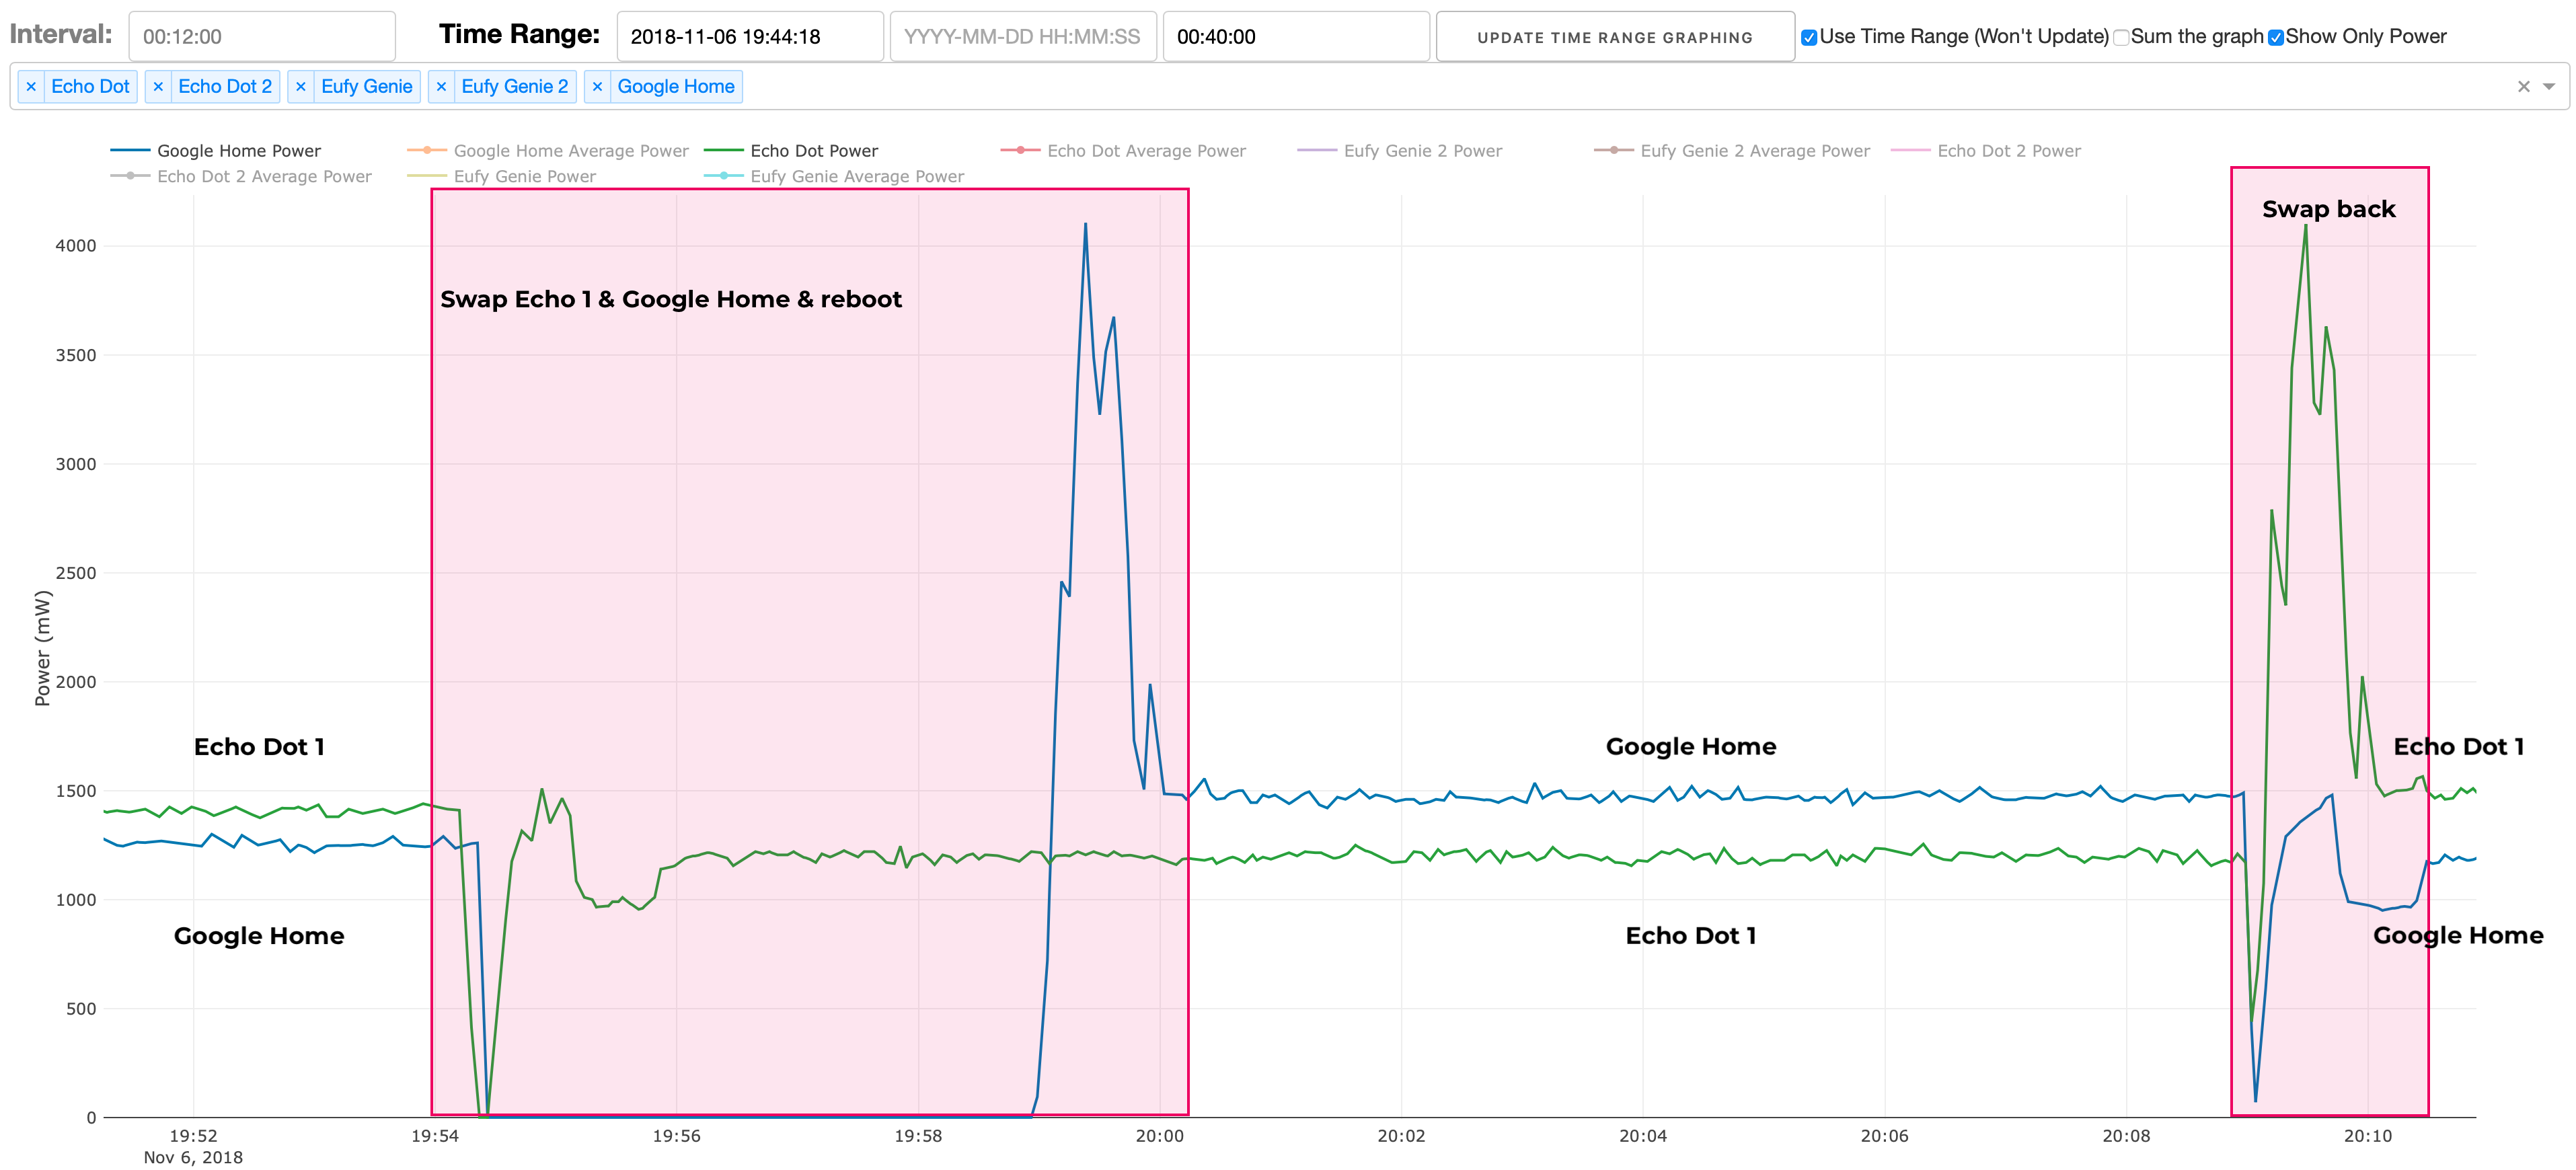
\includegraphics[width=1\textwidth]{figures/swapEcho1Home.png}
    \caption{Connected the Echo Dot 1 to WeMo for `Eufy Genie 1' and vice versa. The traces swap before and after switching.}
    \label{fig:swapEcho1Home}
\end{figure}

\begin{figure}[H]
    \centering
    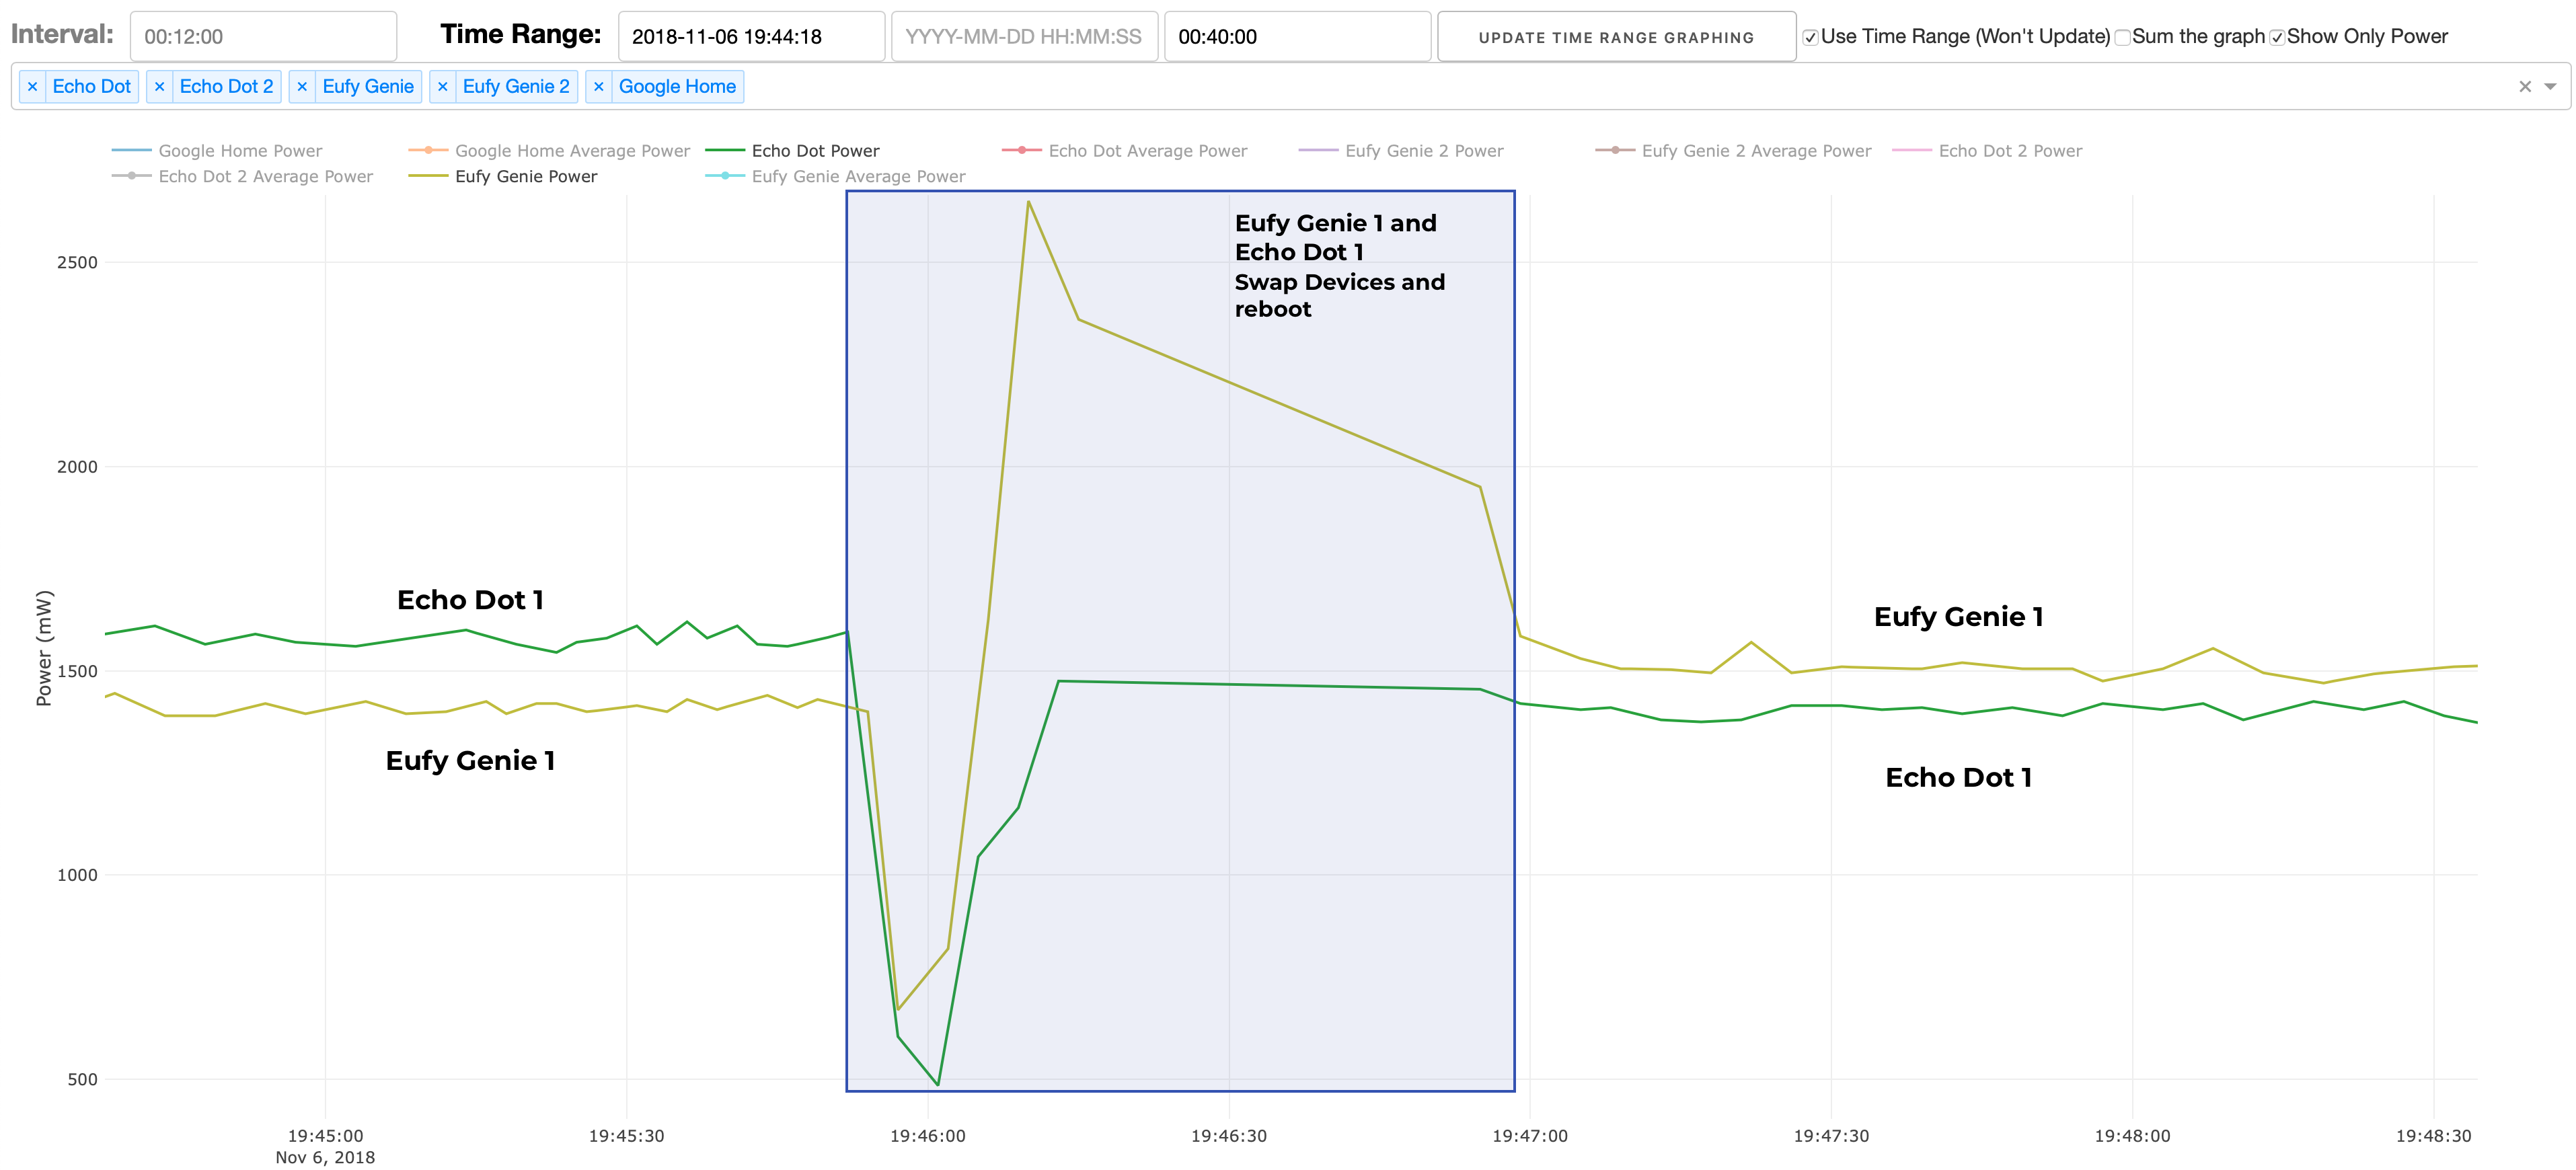
\includegraphics[width=1\textwidth]{figures/swapEufy1Echo1.png}
    \caption{Connected the Eufy Genie 1 to WeMo for `Echo Dot 1' and vice versa. The traces swap before and after switching.}
    \label{fig:swapEufy1Echo1}
\end{figure}

\begin{figure}[H]
    \centering
    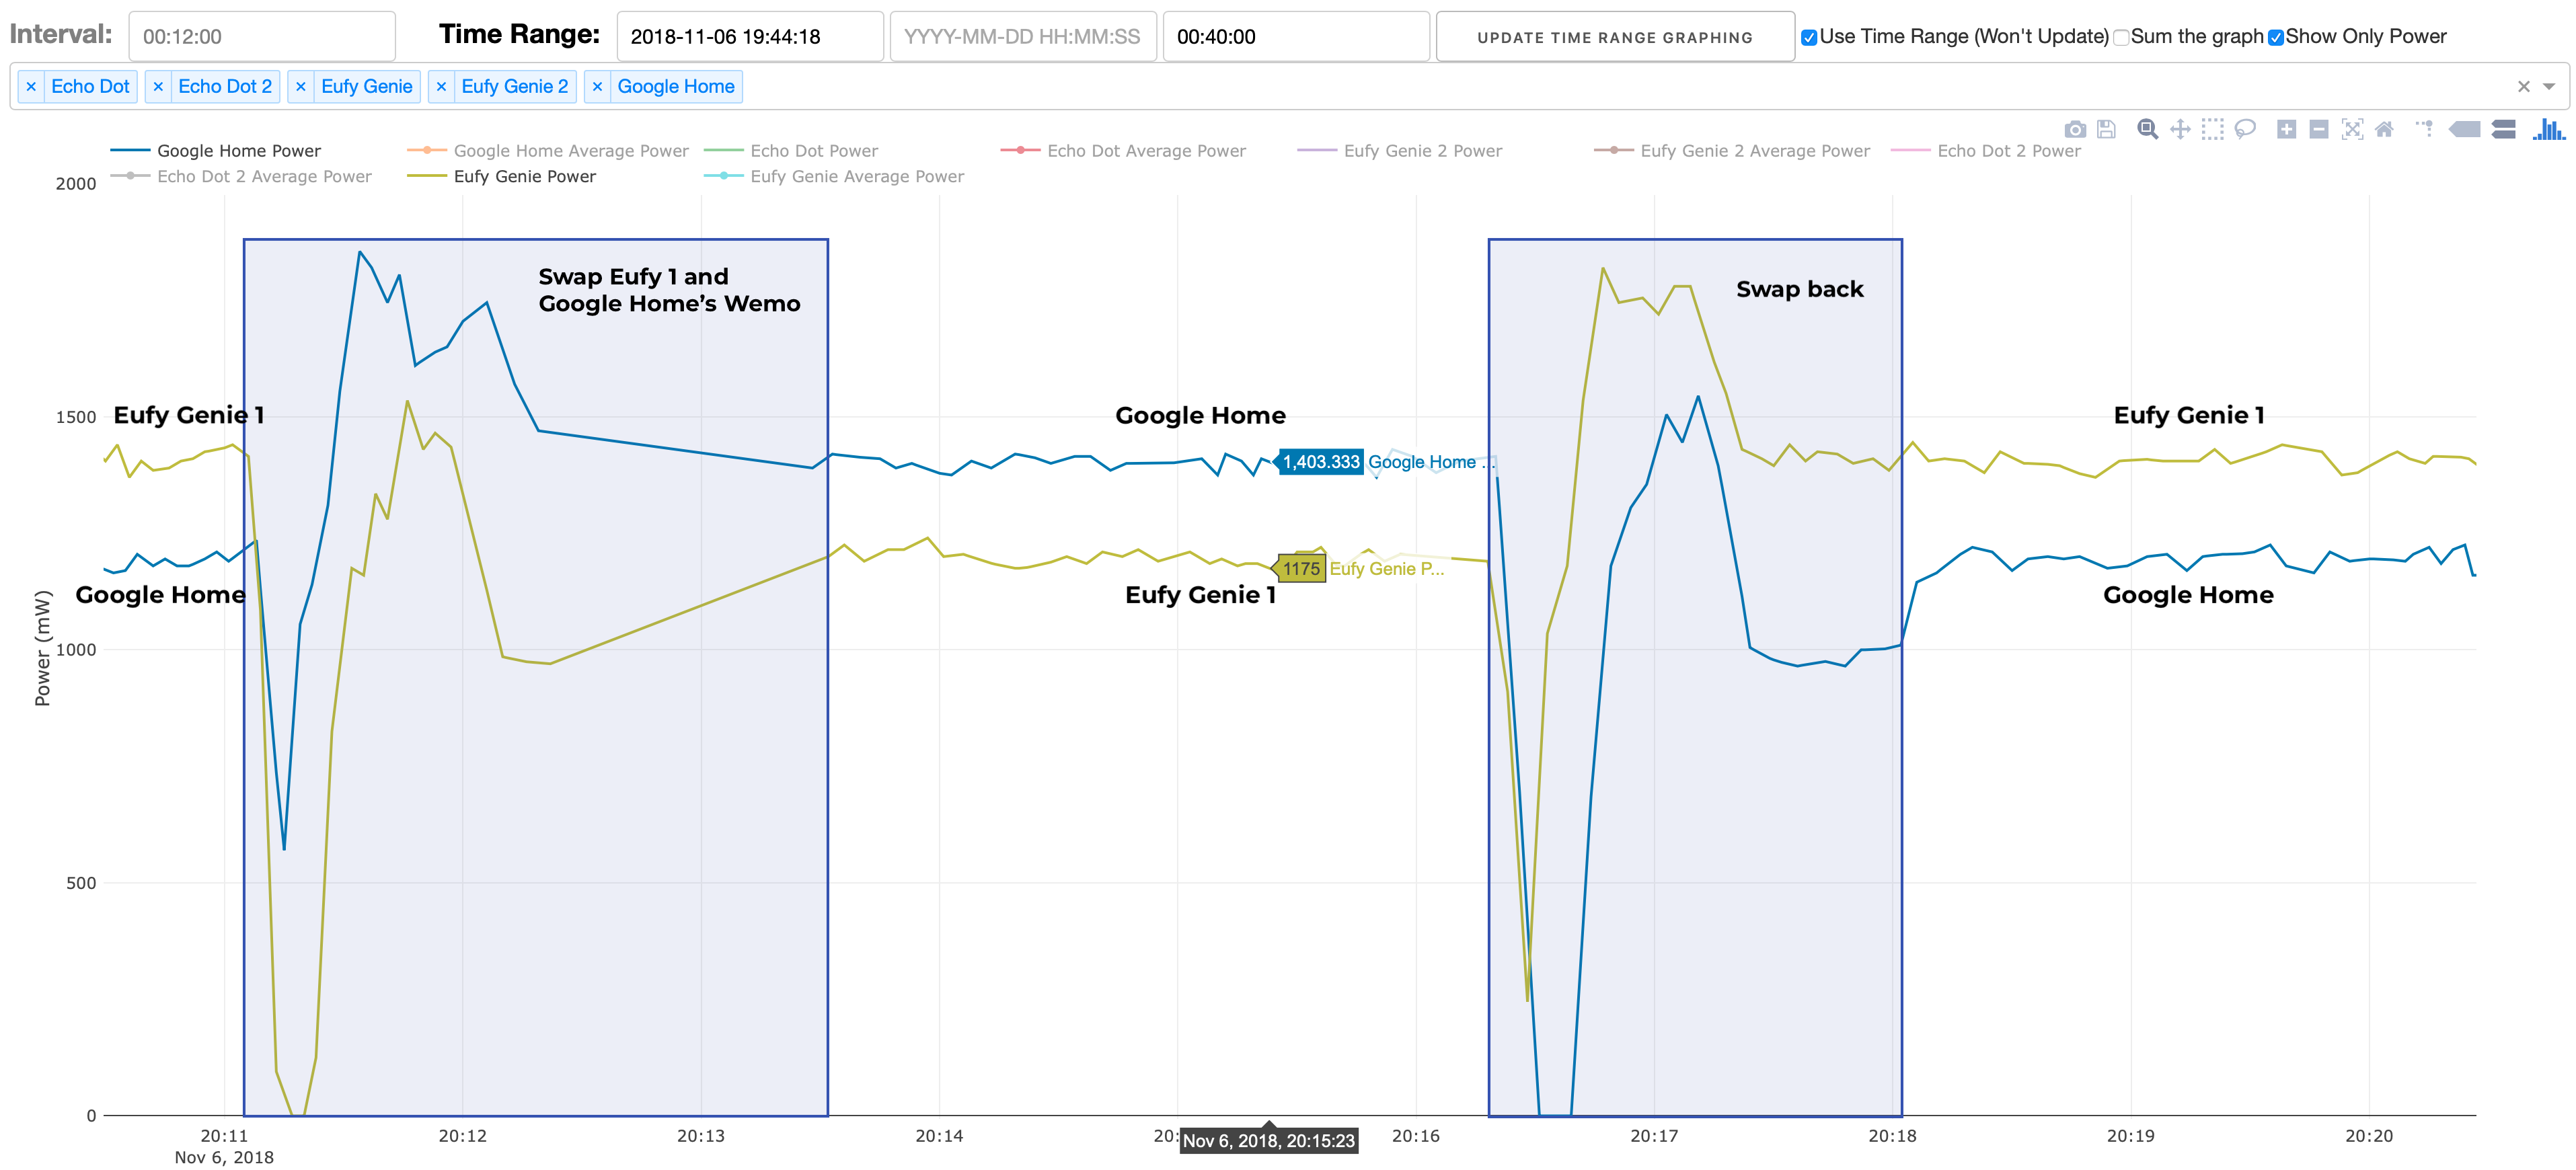
\includegraphics[width=1\textwidth]{figures/swapEufy1Home.png}
    \caption{Connected the Google Home to WeMo for `Eufy Genie 1' and vice versa. The traces swap before and after switching.}
    \label{fig:swapEufy1Home}
\end{figure}

\section{Whole Database}
\label{wholeDB}
When examining the whole database, most of the traffic is TCP packets. The second most significant protocol is UDP. The amount of packets using each protocol are shown in \ref{fig:tcpudp}. This figure is an example of some information that can be acquired from the database.

It shows the percentage of certain protocols that would pass through a typical home, adding to the fingerprint of IoT devices. Refer to Frawley's paper for more information on trends in the whole database\ref{frawleyPaper}.

\label{Whole Database}
\begin{figure}[H]
  \centering
    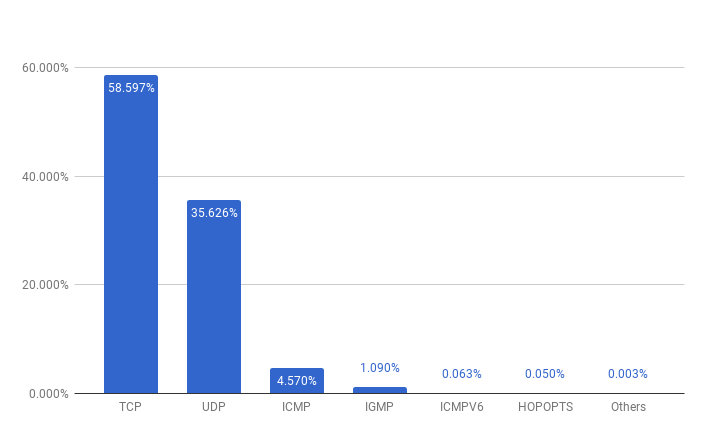
\includegraphics[width=1\textwidth]{tcpudp}
  \caption{Internet and Transport Layer Protocols in Database}
  \label{fig:tcpudp}
\end{figure}

\section{General Analysis}
\label{General Analysis}
The figures shown in this section give examples on how the database and grapher tool can be used. The figures also demonstrate a strong correlation between what the device is doing and its network/power usage, serving as data to fingerprint each smart speaker.

Frawley's paper contains a more in-depth analysis on this section and includes GeoIP \cite{maxmind} information from Cal Poly's ITS servers \cite{its} that highlights the locations and companies the network packets are being sent to and recieved from. Frawley's paper also includes data of unencrypted packets being sent and recieved along with the text within them. The rest of the sections include

\subsection{Smart Speakers}
\label{smartSpeakerResults}
This subsection covers the smart speakers' power and network usage in different scenarios.

\subsubsection{Google Home Mini}
The Google Home Mini's idle traffic broadcasts SSDP (Simple Service Discovery Protocol) packets once every minute. The SSDP packets are a discovery request packet for every IoT device on the network that supports UPnP (Universal Plug and Play). At which point devices such as the Echo Dot, Samsung TV, streaming devices, and the Chromebook respond with information about themselves in a .xml file. This XML file contains details regarding the device operating system and more. Google also sends encrypted TCP packets to Google every 10 minutes. The Google Home Mini's idle traffic is shown in figure \ref{fig:home}. The high peaks are the encrypted TCP packets, and the smaller spikes are the SSDP/UPnP packets.

\begin{figure}[H]
  \centering
    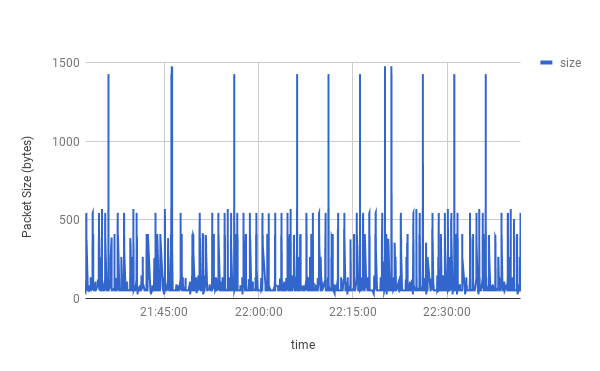
\includegraphics[width=0.9\textwidth]{home1hr}
  \caption{Idle Traffic of Google Home Over 1 Hour Period}
  \label{fig:home}
\end{figure}

A graph of the Google Home Mini's network and power usage under various commands are shown in the figure \ref{fig:homequery}. The Google Home Mini is first asked for the news and then told to stop. After waiting for 40 minutes, we ask it for the weather forecast.

\begin{figure}[H]
  \centering
    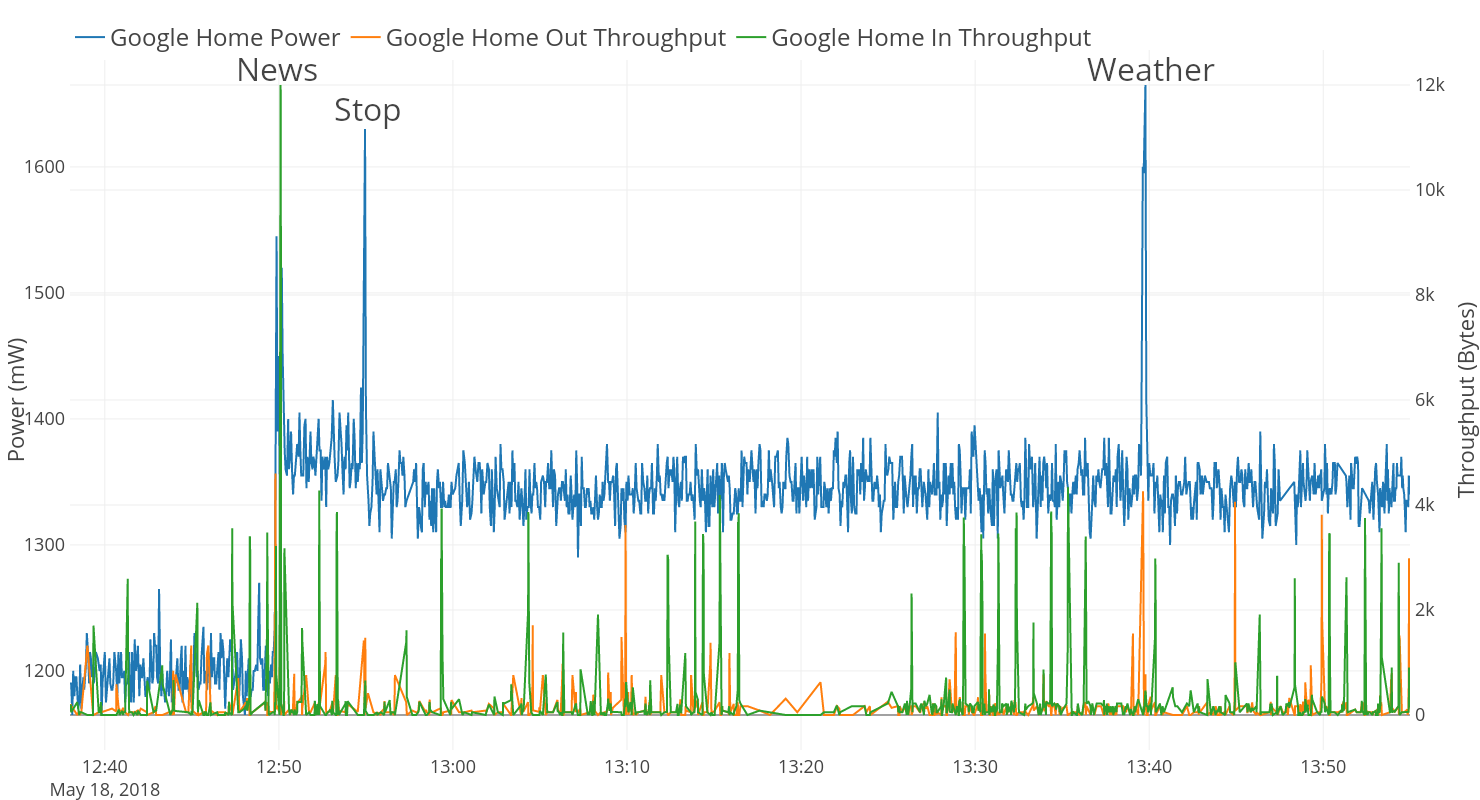
\includegraphics[width=1\textwidth]{homequery}
  \caption{Home Mini Response to News and Weather}
  \label{fig:homequery}
\end{figure}

\subsection{Streaming Devices}
\label{Streaming Devices}
This subsection covers the streaming devices' power and network usage in different scenarios.

\subsubsection{Google Chrome Cast}
\begin{figure}[H]
  \centering
  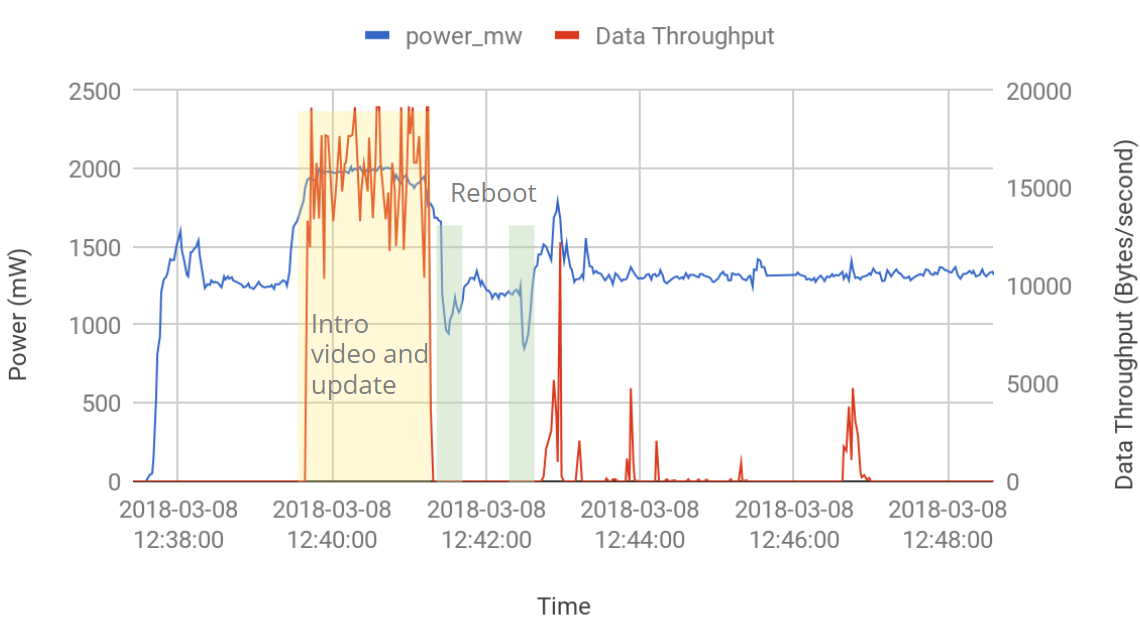
\includegraphics[width=1\textwidth]{ccboth}
  \caption{Chromecast First Time Boot Network Traffic and Power Consumption}
  \label{fig:ccboth}
\end{figure}

The Chrome Cast startup graph is shown in figure \ref{fig:ccboth}. On startup, the Chrome Cast shows an intro tutorial video and downloads a firmware update. After rebooting twice, it is ready to go.

\begin{figure}[H]
  \centering
  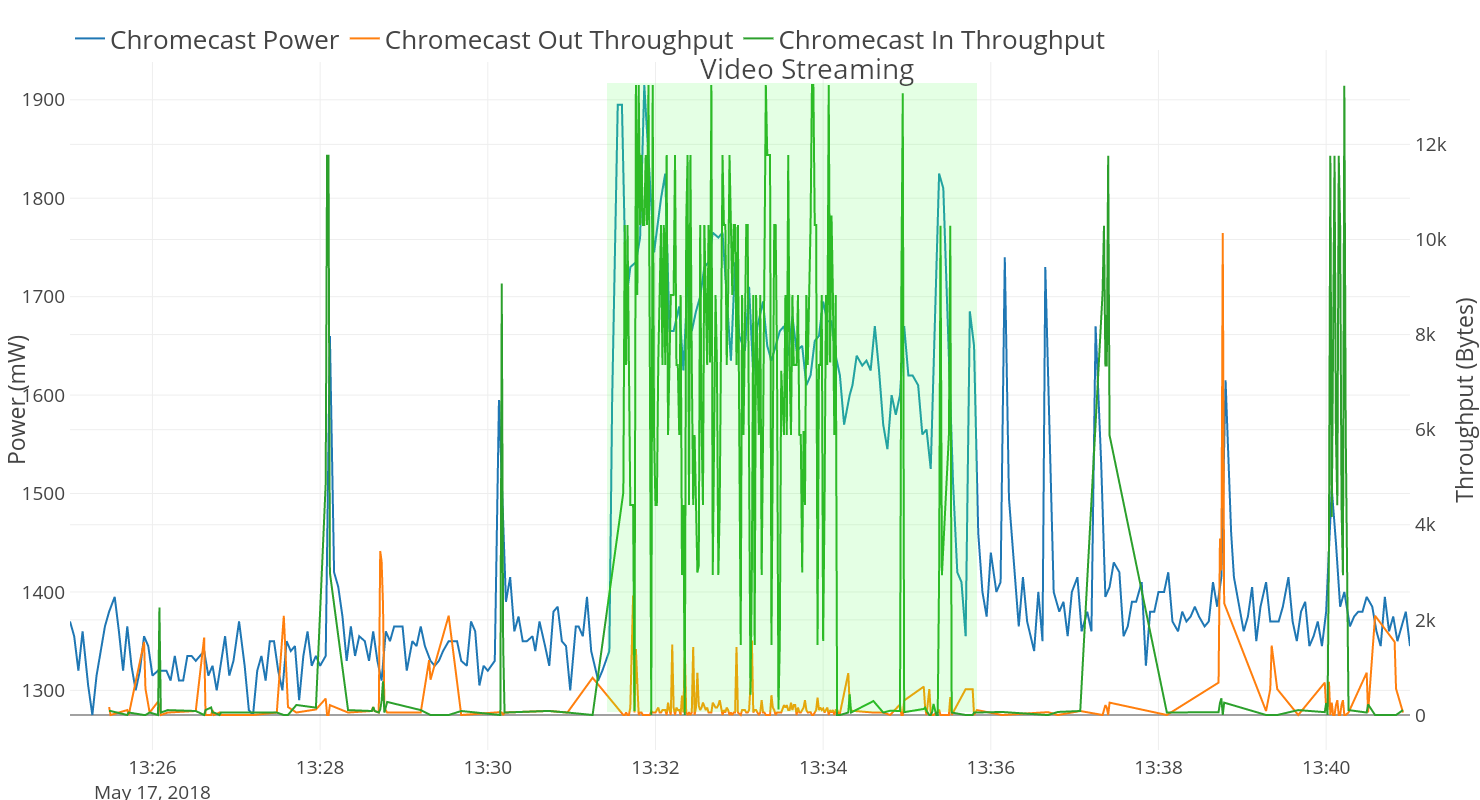
\includegraphics[width=1\textwidth]{ccstreaming}
  \caption{Chromecast Video Streaming}
  \label{fig:ccstream}
\end{figure}

The Chrome Cast streaming graph is shown in figure \ref{fig:ccstream}. In this time frame, the chrome cast streams video in the marked box.

\begin{figure}[H]
  \centering
  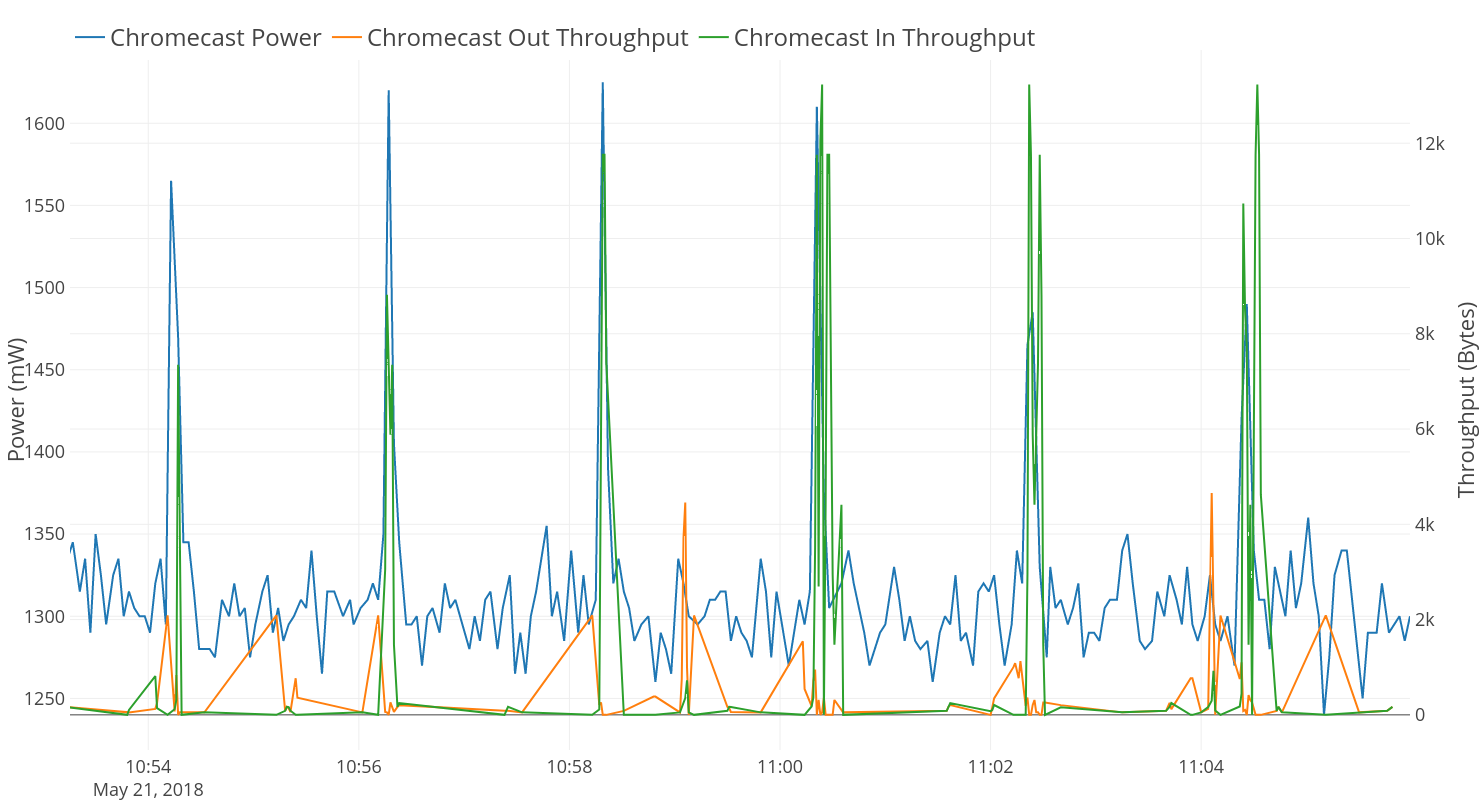
\includegraphics[width=1\textwidth]{chromecastbg}
  \caption{Chromecast Idle Traffic}
  \label{fig:ccbg}
\end{figure}

Additionally, the Chrome Cast idle graph is shown in figure \ref{fig:ccbg}. In this time frame, there are consistent spikes to the chrome cast every 2 minutes. During these spikes, the chrome cast is showing a new background that it downloads from Google Servers.

\subsubsection{Amazon Fire Stick}

\begin{figure}[H]
  \centering
  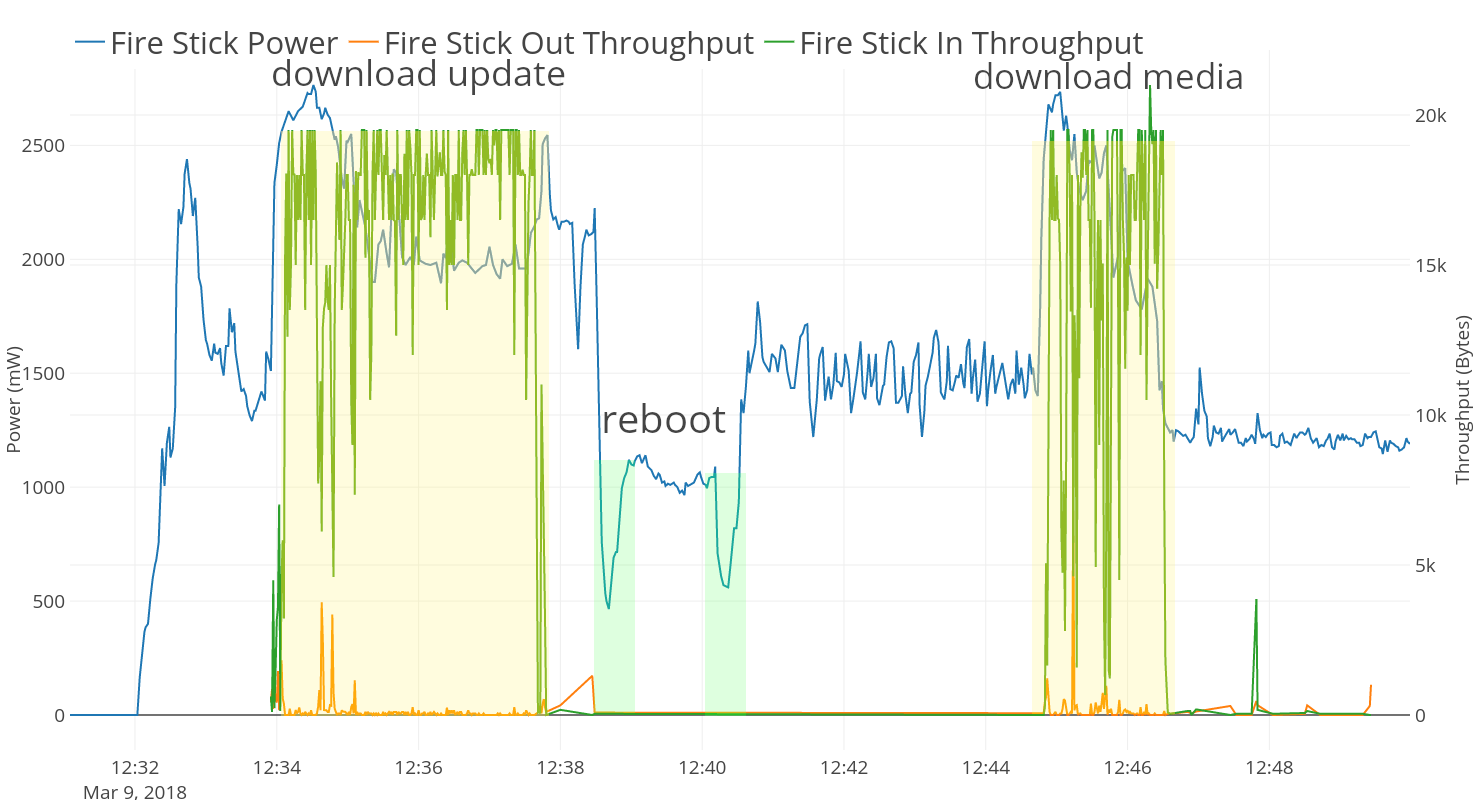
\includegraphics[width=1\textwidth]{fireboot}
  \caption{Fire TV Stick First Time Boot Network Traffic and Power Consumption}
  \label{fig:fireboth}
\end{figure}

The Amazon Fire Stick startup graph is shown in figure \ref{fig:fireboth}. On first boot, the fire stick downloads an update, reboots twice, then downloads certificates from Symantec and Verisign.

When streaming, the Fire Stick increases throughput and power usage with a spike at the beginning and end of streaming in power usage as shown in figure \ref{fig:fsyt}.

\begin{figure}[H]
  \centering
  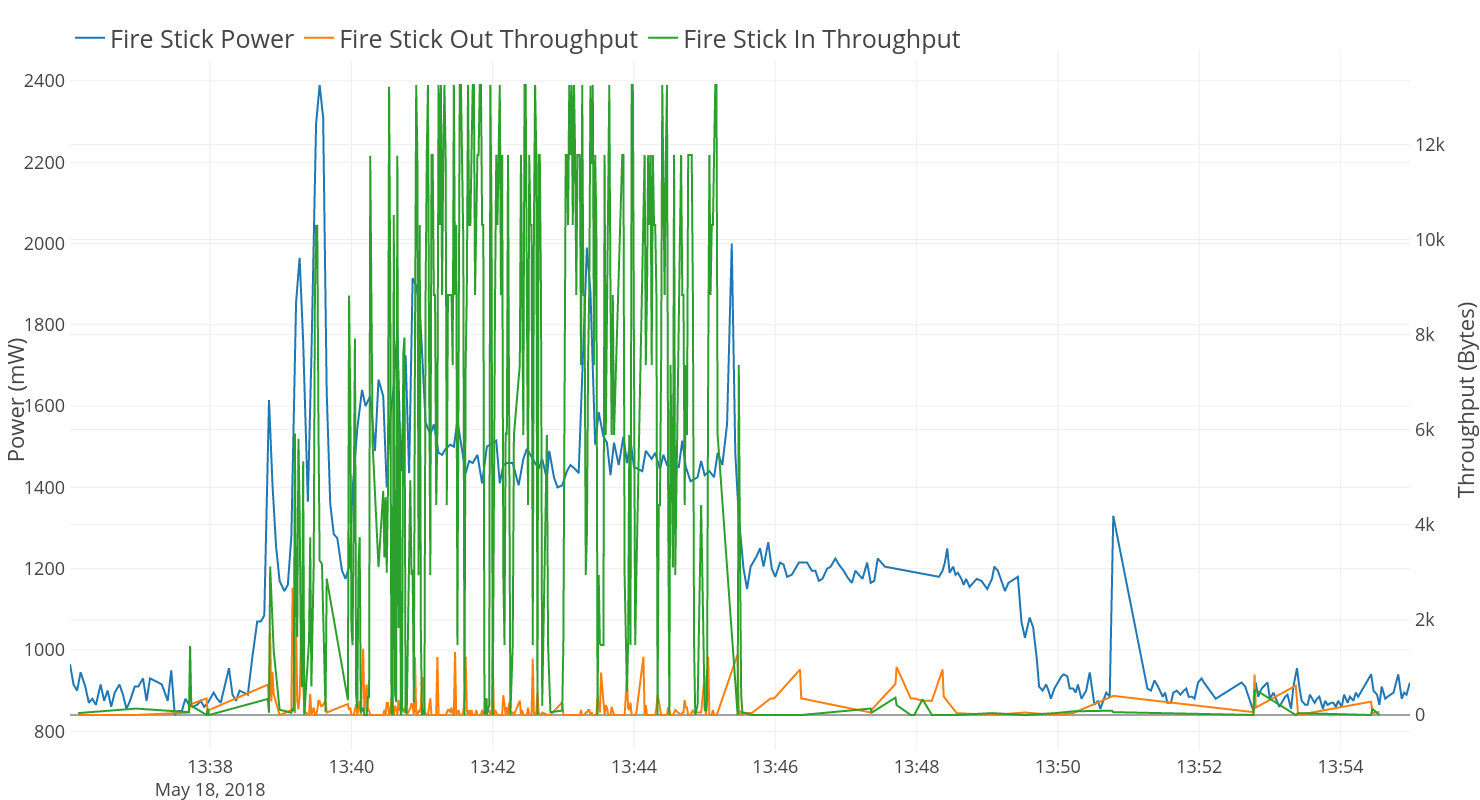
\includegraphics[width=1\textwidth]{fsyt}
  \caption{Fire TV Stick Video Streaming}
  \label{fig:fsyt}
\end{figure}

\subsubsection{Roku Express}
When streaming, the Roku's power usage and network throughput rise and stay at a constant level until the video streaming is complete. At which point it drops back down when done.

\begin{figure}[H]
  \centering
  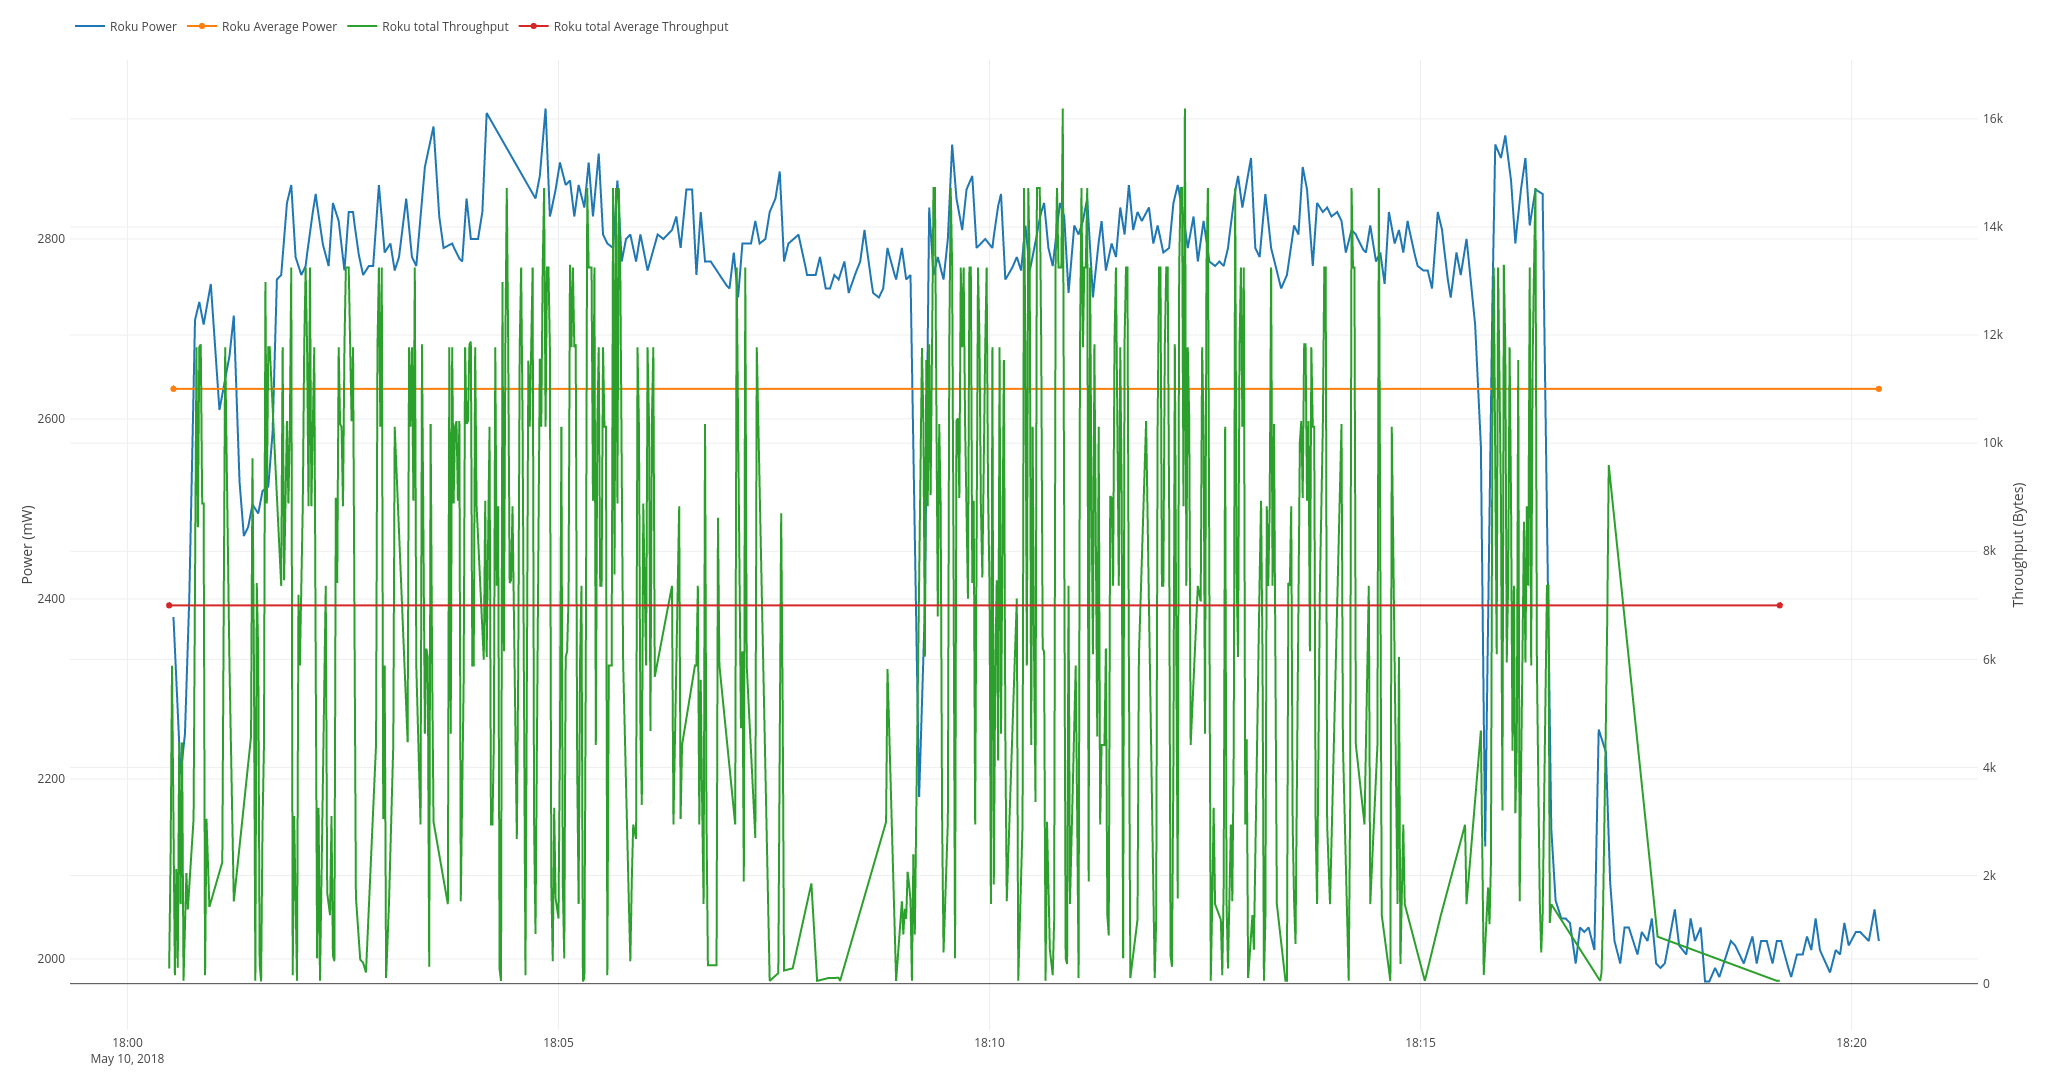
\includegraphics[width=1\textwidth]{figures/rokuStreaming.png}
  \caption{Roku Express Video Streaming}
  \label{fig:rokuStreaming}
\end{figure}

\subsection{General Analysis Discussion}
From all the figures in this section, there is a visual correlation between network/power usage and what the devices is doing. During periodic updates the smart speakers and streamign devices would have periodic network/power usage spikes. While streaming, the power/network usage would increase for the period of the stream. This strong correlation was the first steps in using the database and visualizer tool for visual pattern recognition, proving its viability.

\section{Power Analysis on Smart Speakers}

After determining a strong correlation between network/power usage to device operation, this section begins to focus on power usage over time. Significant analysis on network usage had already been done as shown in the previous works \ref{Previous Work} section. This section highlights initial power findings which shows that a lot can be determined from visually examing a power graph over time in subsection \ref{Echo Dot Brightness Sensor}. Once discovering the insight a power trace can provide, the research focused on overarching goal to see if given a graph of a house's total power usage, is it possible to determine the device in use. This paper will focus on smart speakers' power usage to test this hypotheses.

But before doing that, this section examines the power usage of the smart speakers seperately before examining total power usage in section \ref{sumPowerGraph}. Subsection \ref{Baseline Speaker Power} examines idle power of smart speakers seperately, showing that a smart speaker can be determined from its idle power (to a small extent). Then subsection \ref{Smart Speaker Power Spikes When Asked for Weather} shows that through visual examination of a power trace of an individual smart speaker, we can tell what smart speaker is in use.

\subsection{Echo Dot Brightness Sensor}
\label{Echo Dot Brightness Sensor}
One interesting finding from the Echo Dot is that it has a light monitor. When turning on the lights, the LEDs on the Echo Dot brighten to adapt. The brightness change causes the Echo Dot to use more idle power as shown in figure \ref{fig:echolights}.

Figure \ref{fig:echolights} shows that the power usage of an Echo Dot can show if the lights are on in a house. This can help someone determine if someone is in their house or not or event what room they are in, introducing some privacy concerns.

\begin{figure}[H]
    \centering
    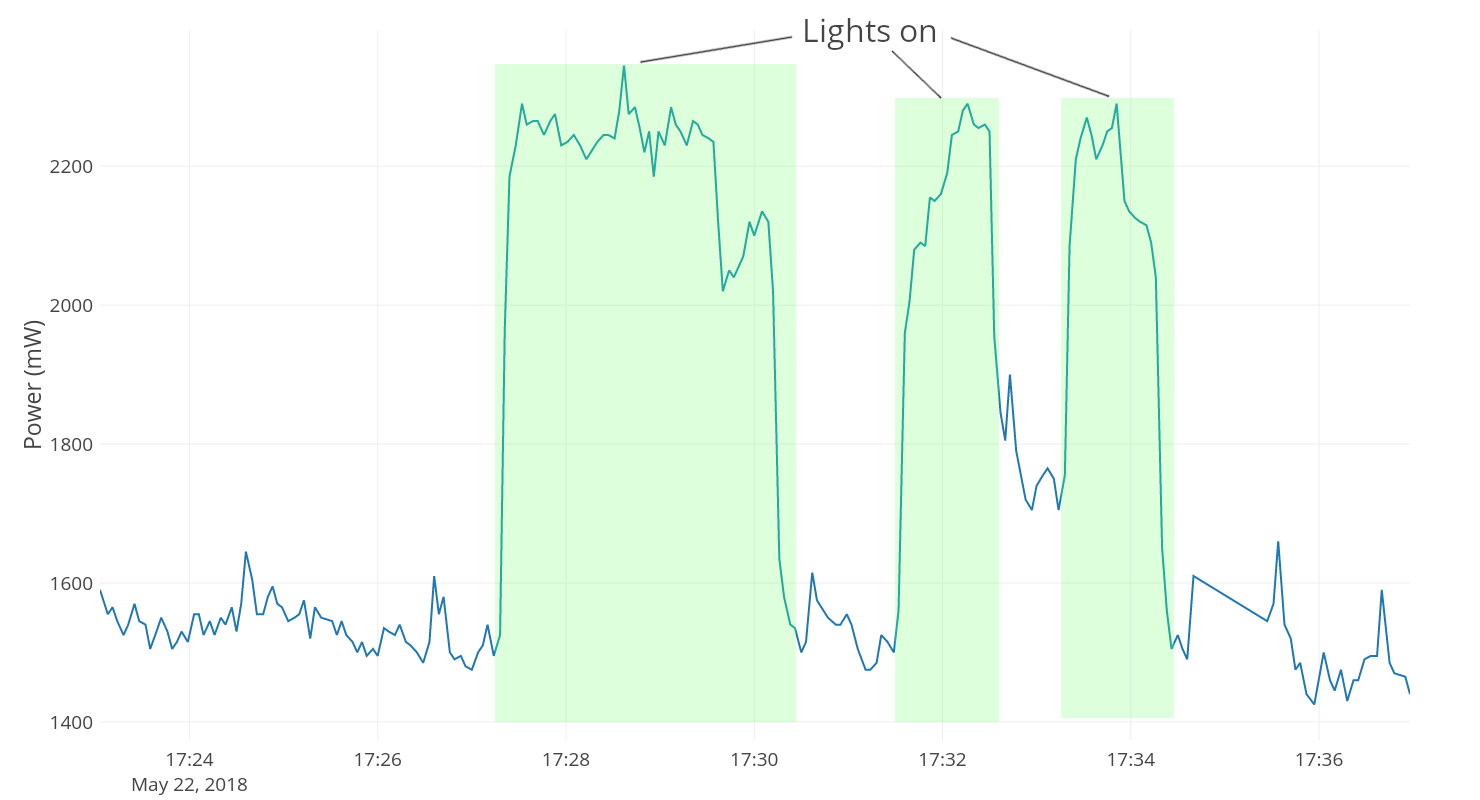
\includegraphics[width=1\textwidth]{echolights}
    \caption{Echo Dot Response to Lights}
    \label{fig:echolights}
\end{figure}

\subsection{Baseline Speaker Power}
\label{Baseline Speaker Power}
Once discovering how much a smart speaker's power usage can show, this section examines the power usage of each smart speaker while idle. Figure \ref{fig:baselineSpeakerPower} shows this from 1:00 AM to 2:30 AM when none of the devices are in use.

The Echo Dot 1 has the highest idle traffic as shown in the pink trace, the Echo Dot 2 has second highest idle traffic as shown in the green trace, the Eufy 1 and Eufy 2 have the same idle power usage as shown in the yellow and purple trace, then the Google Home has the lowest idle power usage as shown in the blue trace. With visual analysis, thesmart speaker can be matched to idle power usage. But the power usages can overlap between the Echo Dot 2 and Eufys. This would make it difficult to differentiate them and proves this method of device determination difficult. Also, when summing the power usages together, these idle traces would dissapear, with no way to differntiate what idle devices are contributing to the total power usage.

\begin{figure}[H]
    \centering
    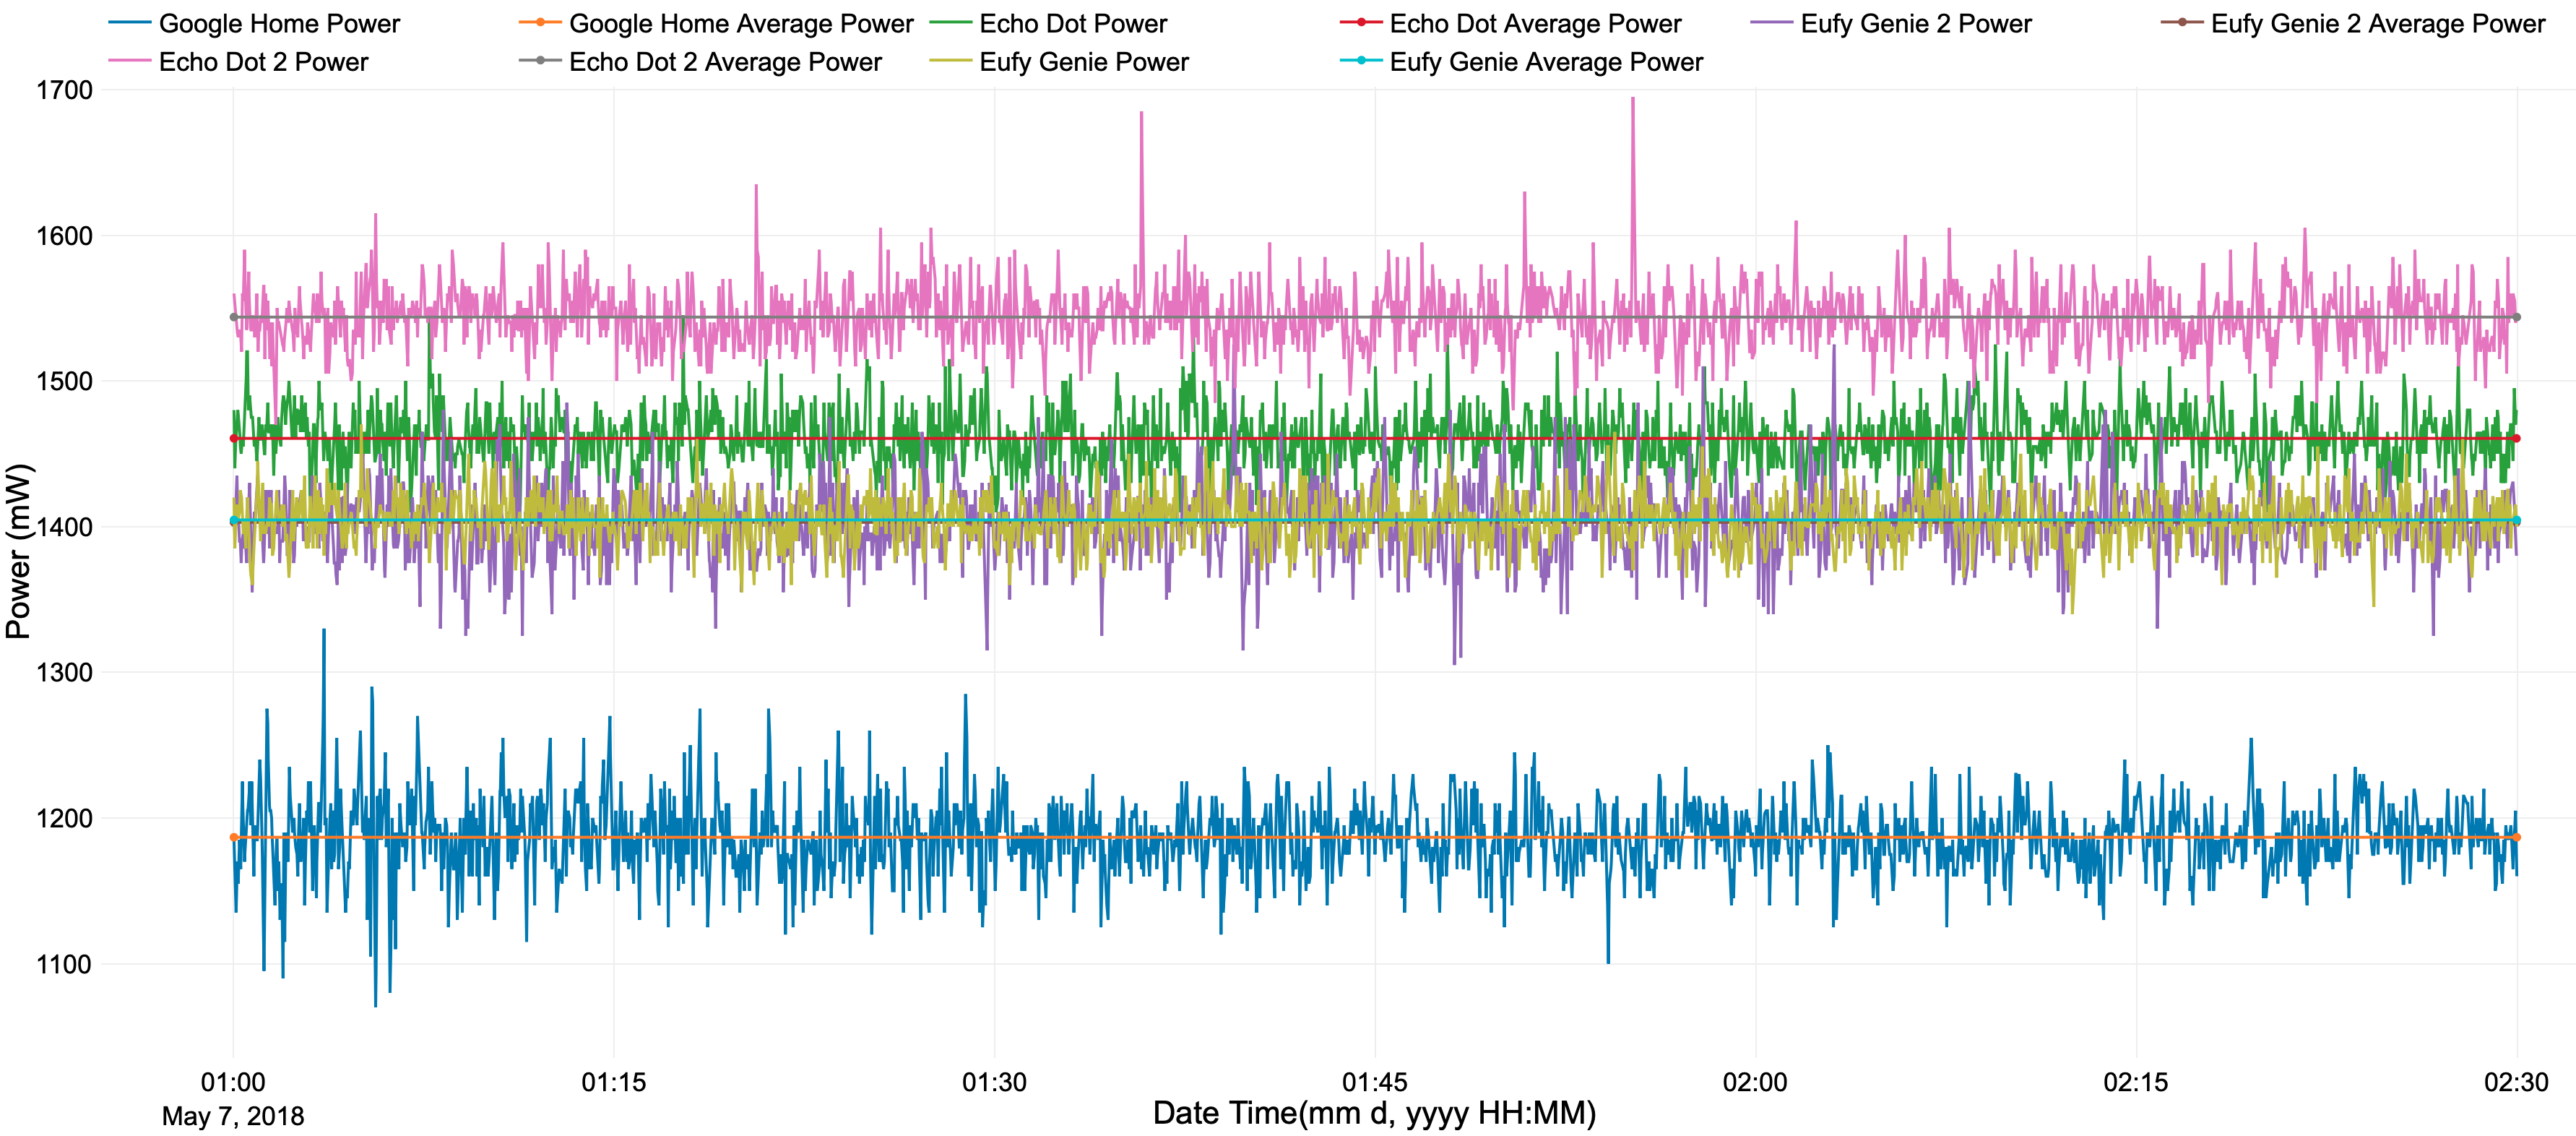
\includegraphics[width=1\textwidth]{baselineSpeakerPower.png}
    \caption{Baseline smart speaker power usage.}
    \label{fig:baselineSpeakerPower}
\end{figure}

\subsection{Smart Speaker Power Spikes When Asked for Weather}
\label{Smart Speaker Power Spikes When Asked for Weather}
This section continues to see if a smart speaker can be determined from an individual power trace, focusing on traces while the device is in use. This is shown in figure \ref{fig:speakerWeatherSeperate} where each device is asked for the weather 4 times.

In figure \ref{fig:speakerWeatherSeperate} there is a visual spike for each device while it is giving the weather forecast. Each device is highlighted while in use, showing 4 spikes. The Google Home was queried for the weather 5 times, thus containing an extra spike. From this, we can determine a Eufy trace if it has small 400 mW spikes, the Google Home if there are medium 600 mW spikes, and the Echo Dot if there are large 2,100 mW spikes. This implies that a device can be determined from a power trace if the device is asked for the weather. In the next section, more use cases are analyzed and the traces are summed together to more closely simulate a shared home powerline.

\begin{figure}[H]
    \centering
    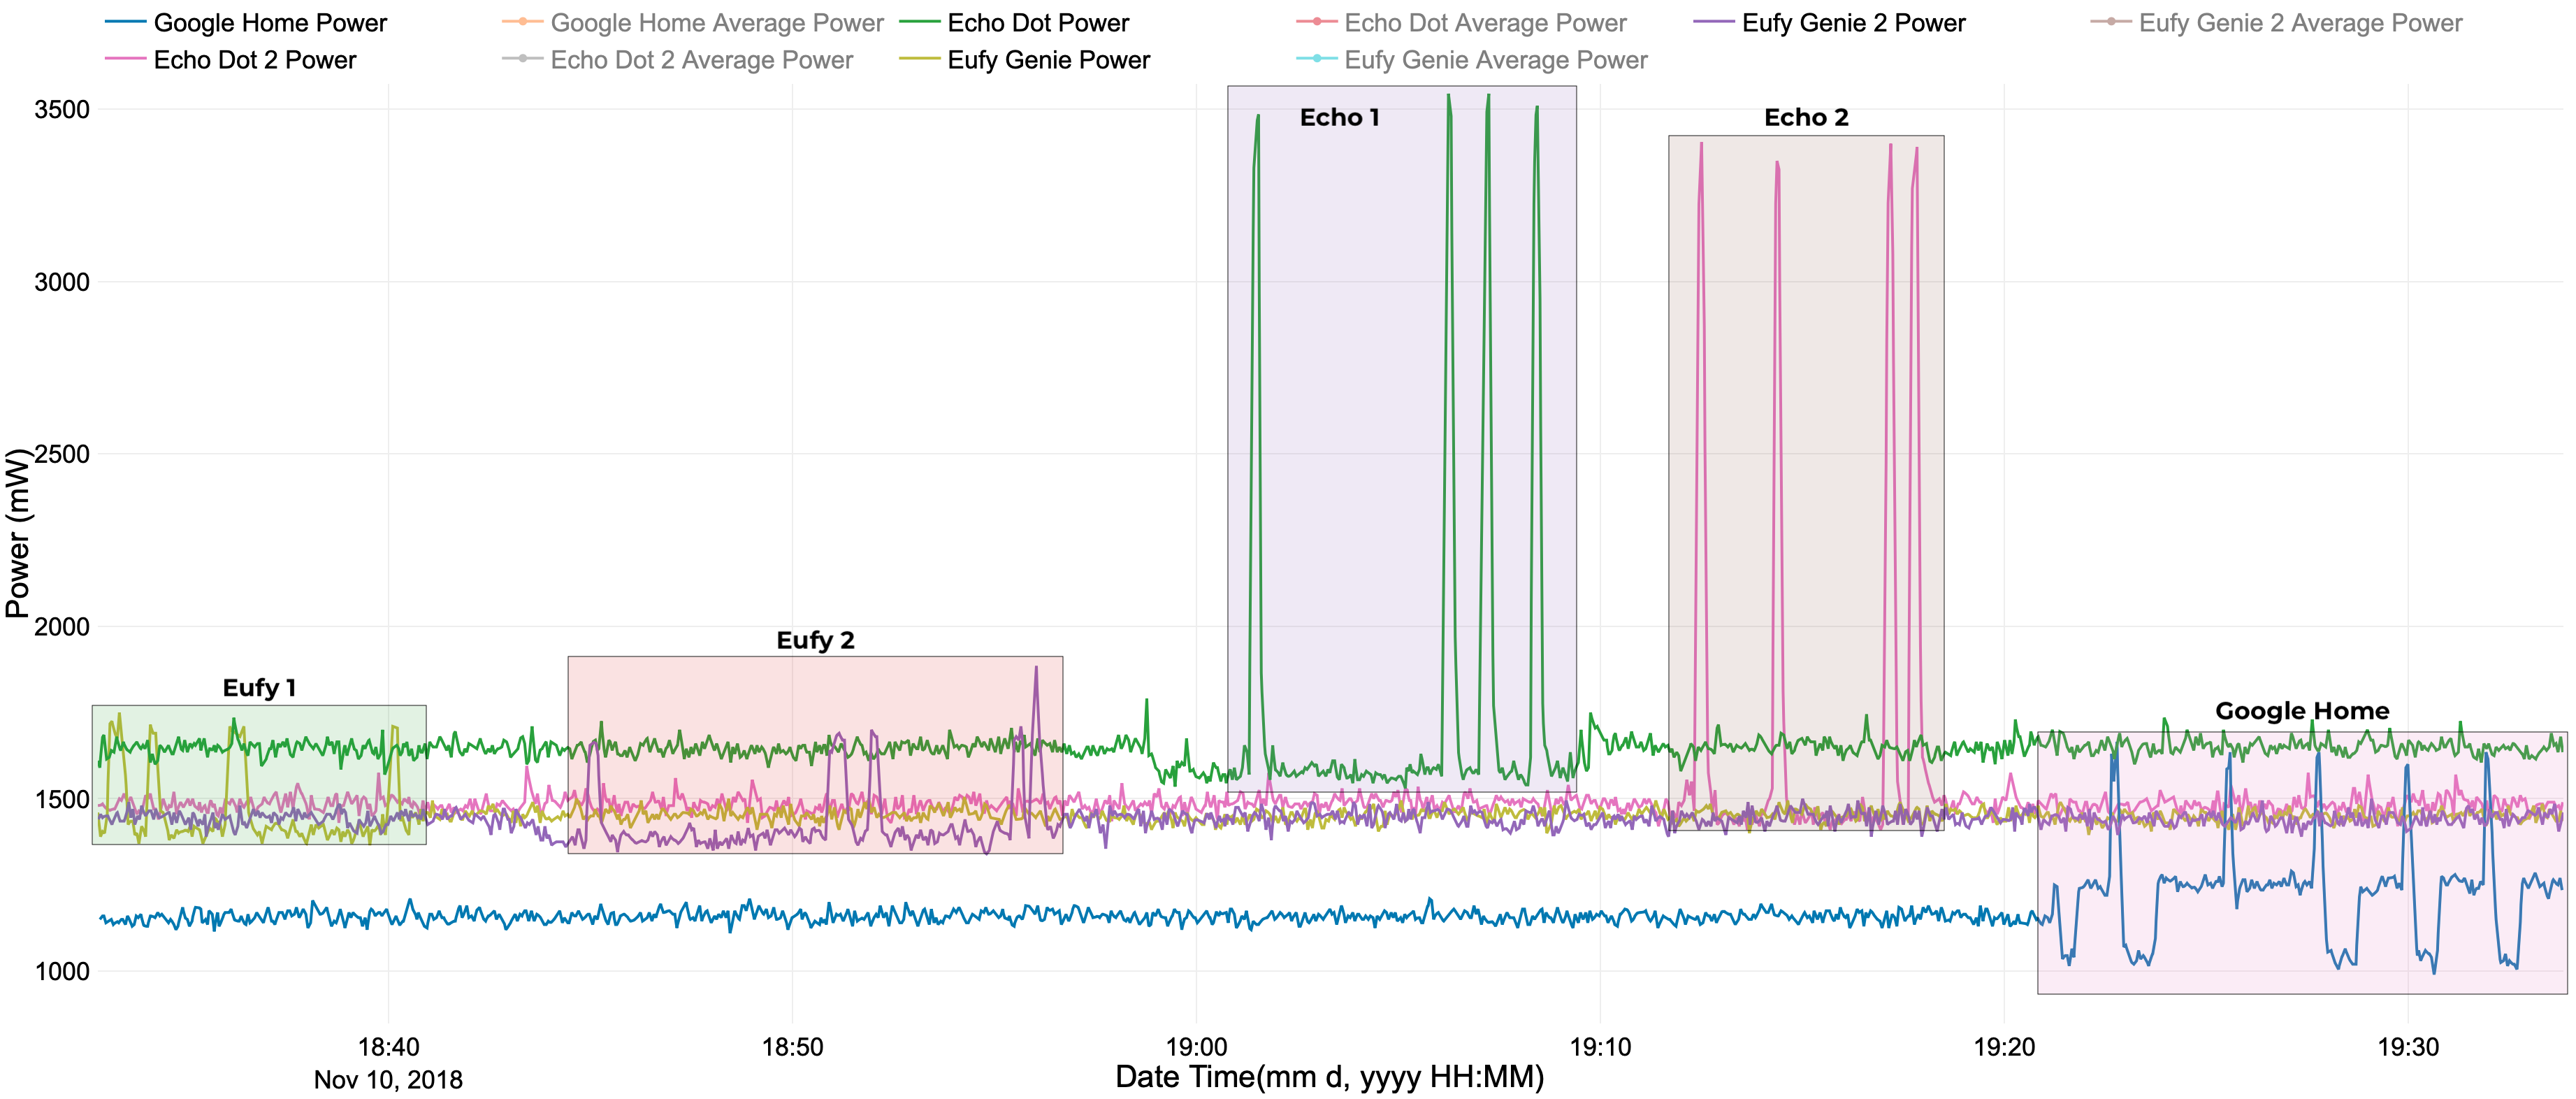
\includegraphics[width=1\textwidth]{speakerWeatherSeperate.png}
    \caption{Smart speakers' power usage when asked `what\'s the weather' four times.}
    \label{fig:speakerWeatherSeperate}
\end{figure}

\section{Summed Power Graph}
\label{sumPowerGraph}
This section visually analyzes the power usages of all 5 of the smart speakers summed together under different commands.

The first graph in figure \ref{fig:weatherSum} is shown in a time frame where each device was unmuted and muted for a period. This shows if muting and unmuting the devices affected the power or network usage. There are changes on the first runthrough, but when repeating the process nothing happens. Further runthroughs show that the power usage stayed the same. In the last half of the graph we queried each smart speaker for the weather while all other smart speakers were muted at the 18:30 mark. We query each device 3-4 times for the weather. The Eufy had the smallest spike for the ``what\'s the weather'' command at 400 mW, then the google home at 600 mW, and finally the echo dot at 2000 mW.

\begin{figure}[H]
  \centering
  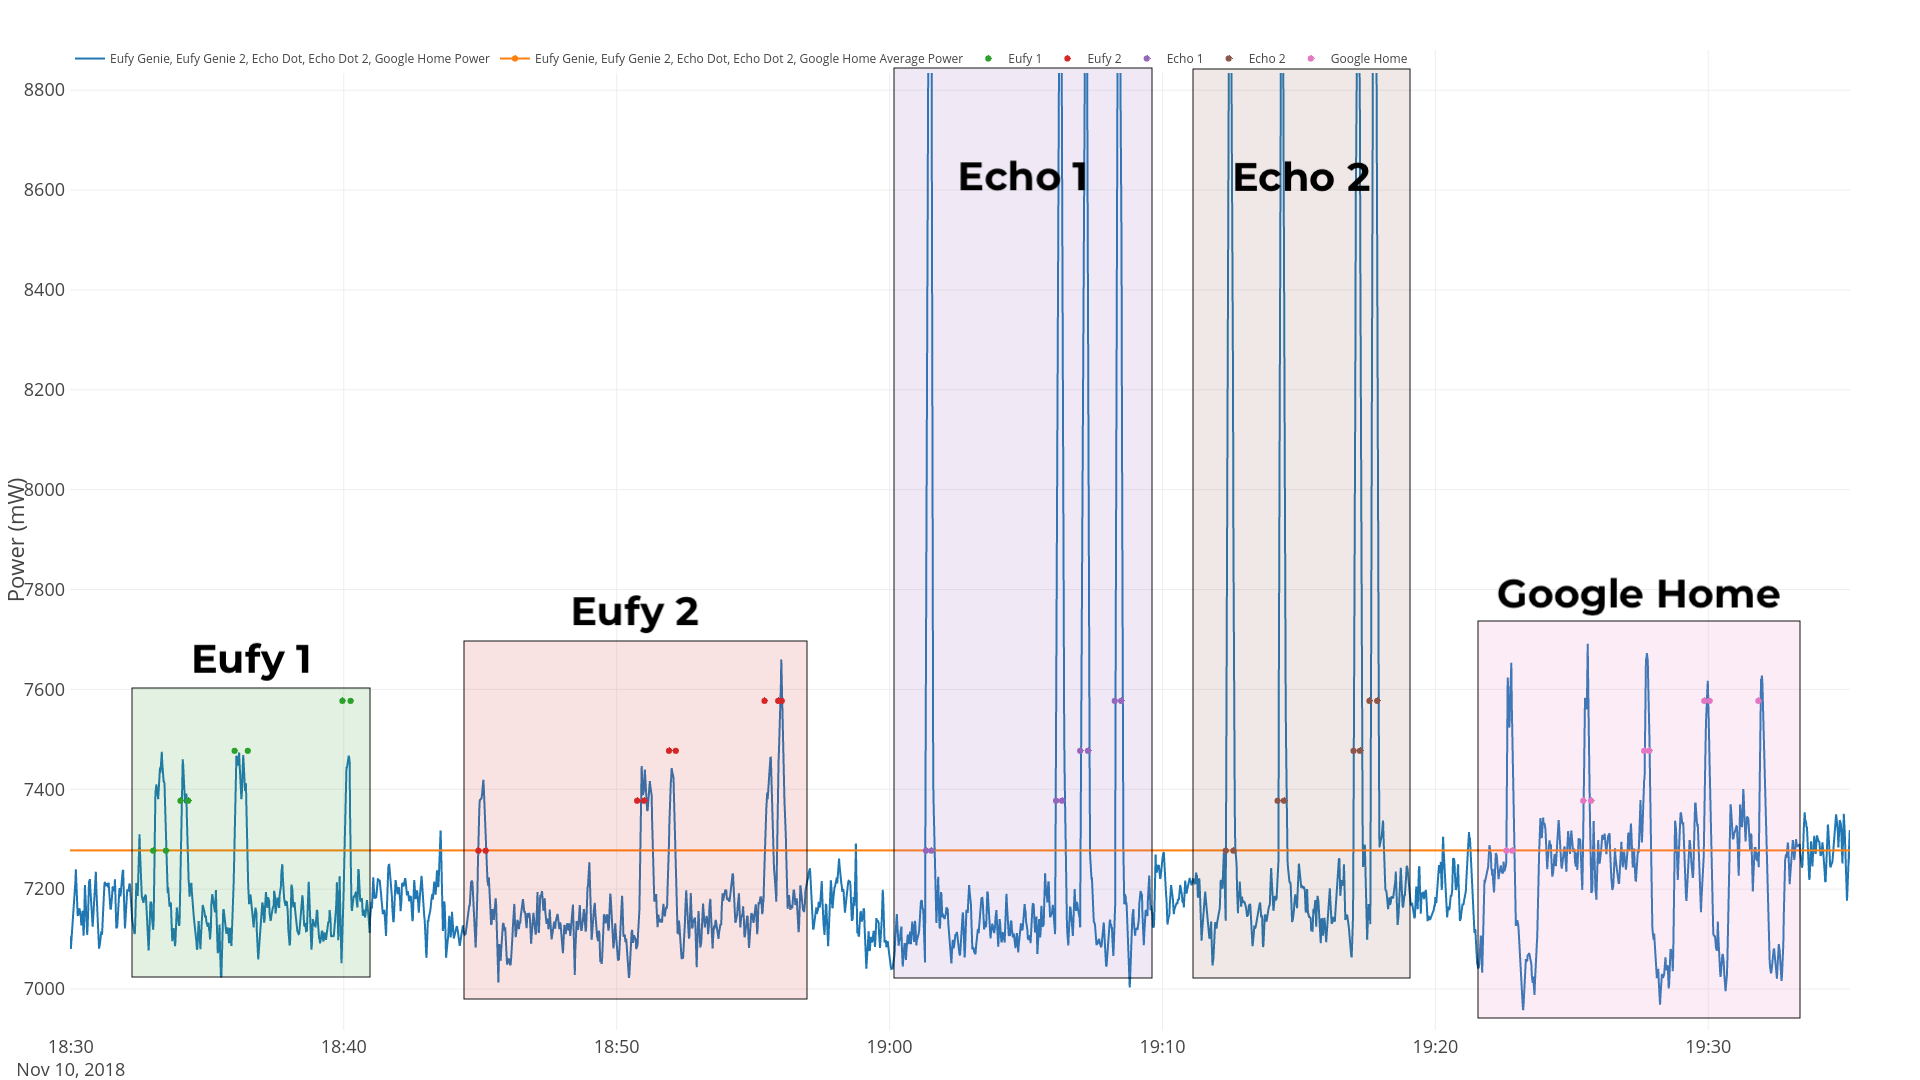
\includegraphics[width=1\textwidth]{figures/weatherSum.png}
  \caption{5 Smart Speakers Power Summed Up. Toggled the mute button and queried each device for the weather.}
  \label{fig:weatherSum}
\end{figure}

The next graph, \ref{fig:mixedNewsSum}, shows the smart speakers power usage when asked for the news. Each speaker was asked for the news. This graph and the rest of the summed graphs in this section use the same notation for signifying commands. Two corresponding dots of the same color signify the start and end of the command for a specific device. If the dots are on another level, then this command has been repeated another time.

In figure \ref{fig:mixedNewsSum}, all devices have a spike at the beginning and end of the command and maintain a steady energy usage in between that is slightly higher than the idle energy used. The peak to peak spike of the Eufy Genie is the smallest at 350 mW, then the Google Home at 500 mW, and finally the Echo Dot at 1900 mW.

\begin{figure}[H]
  \centering
  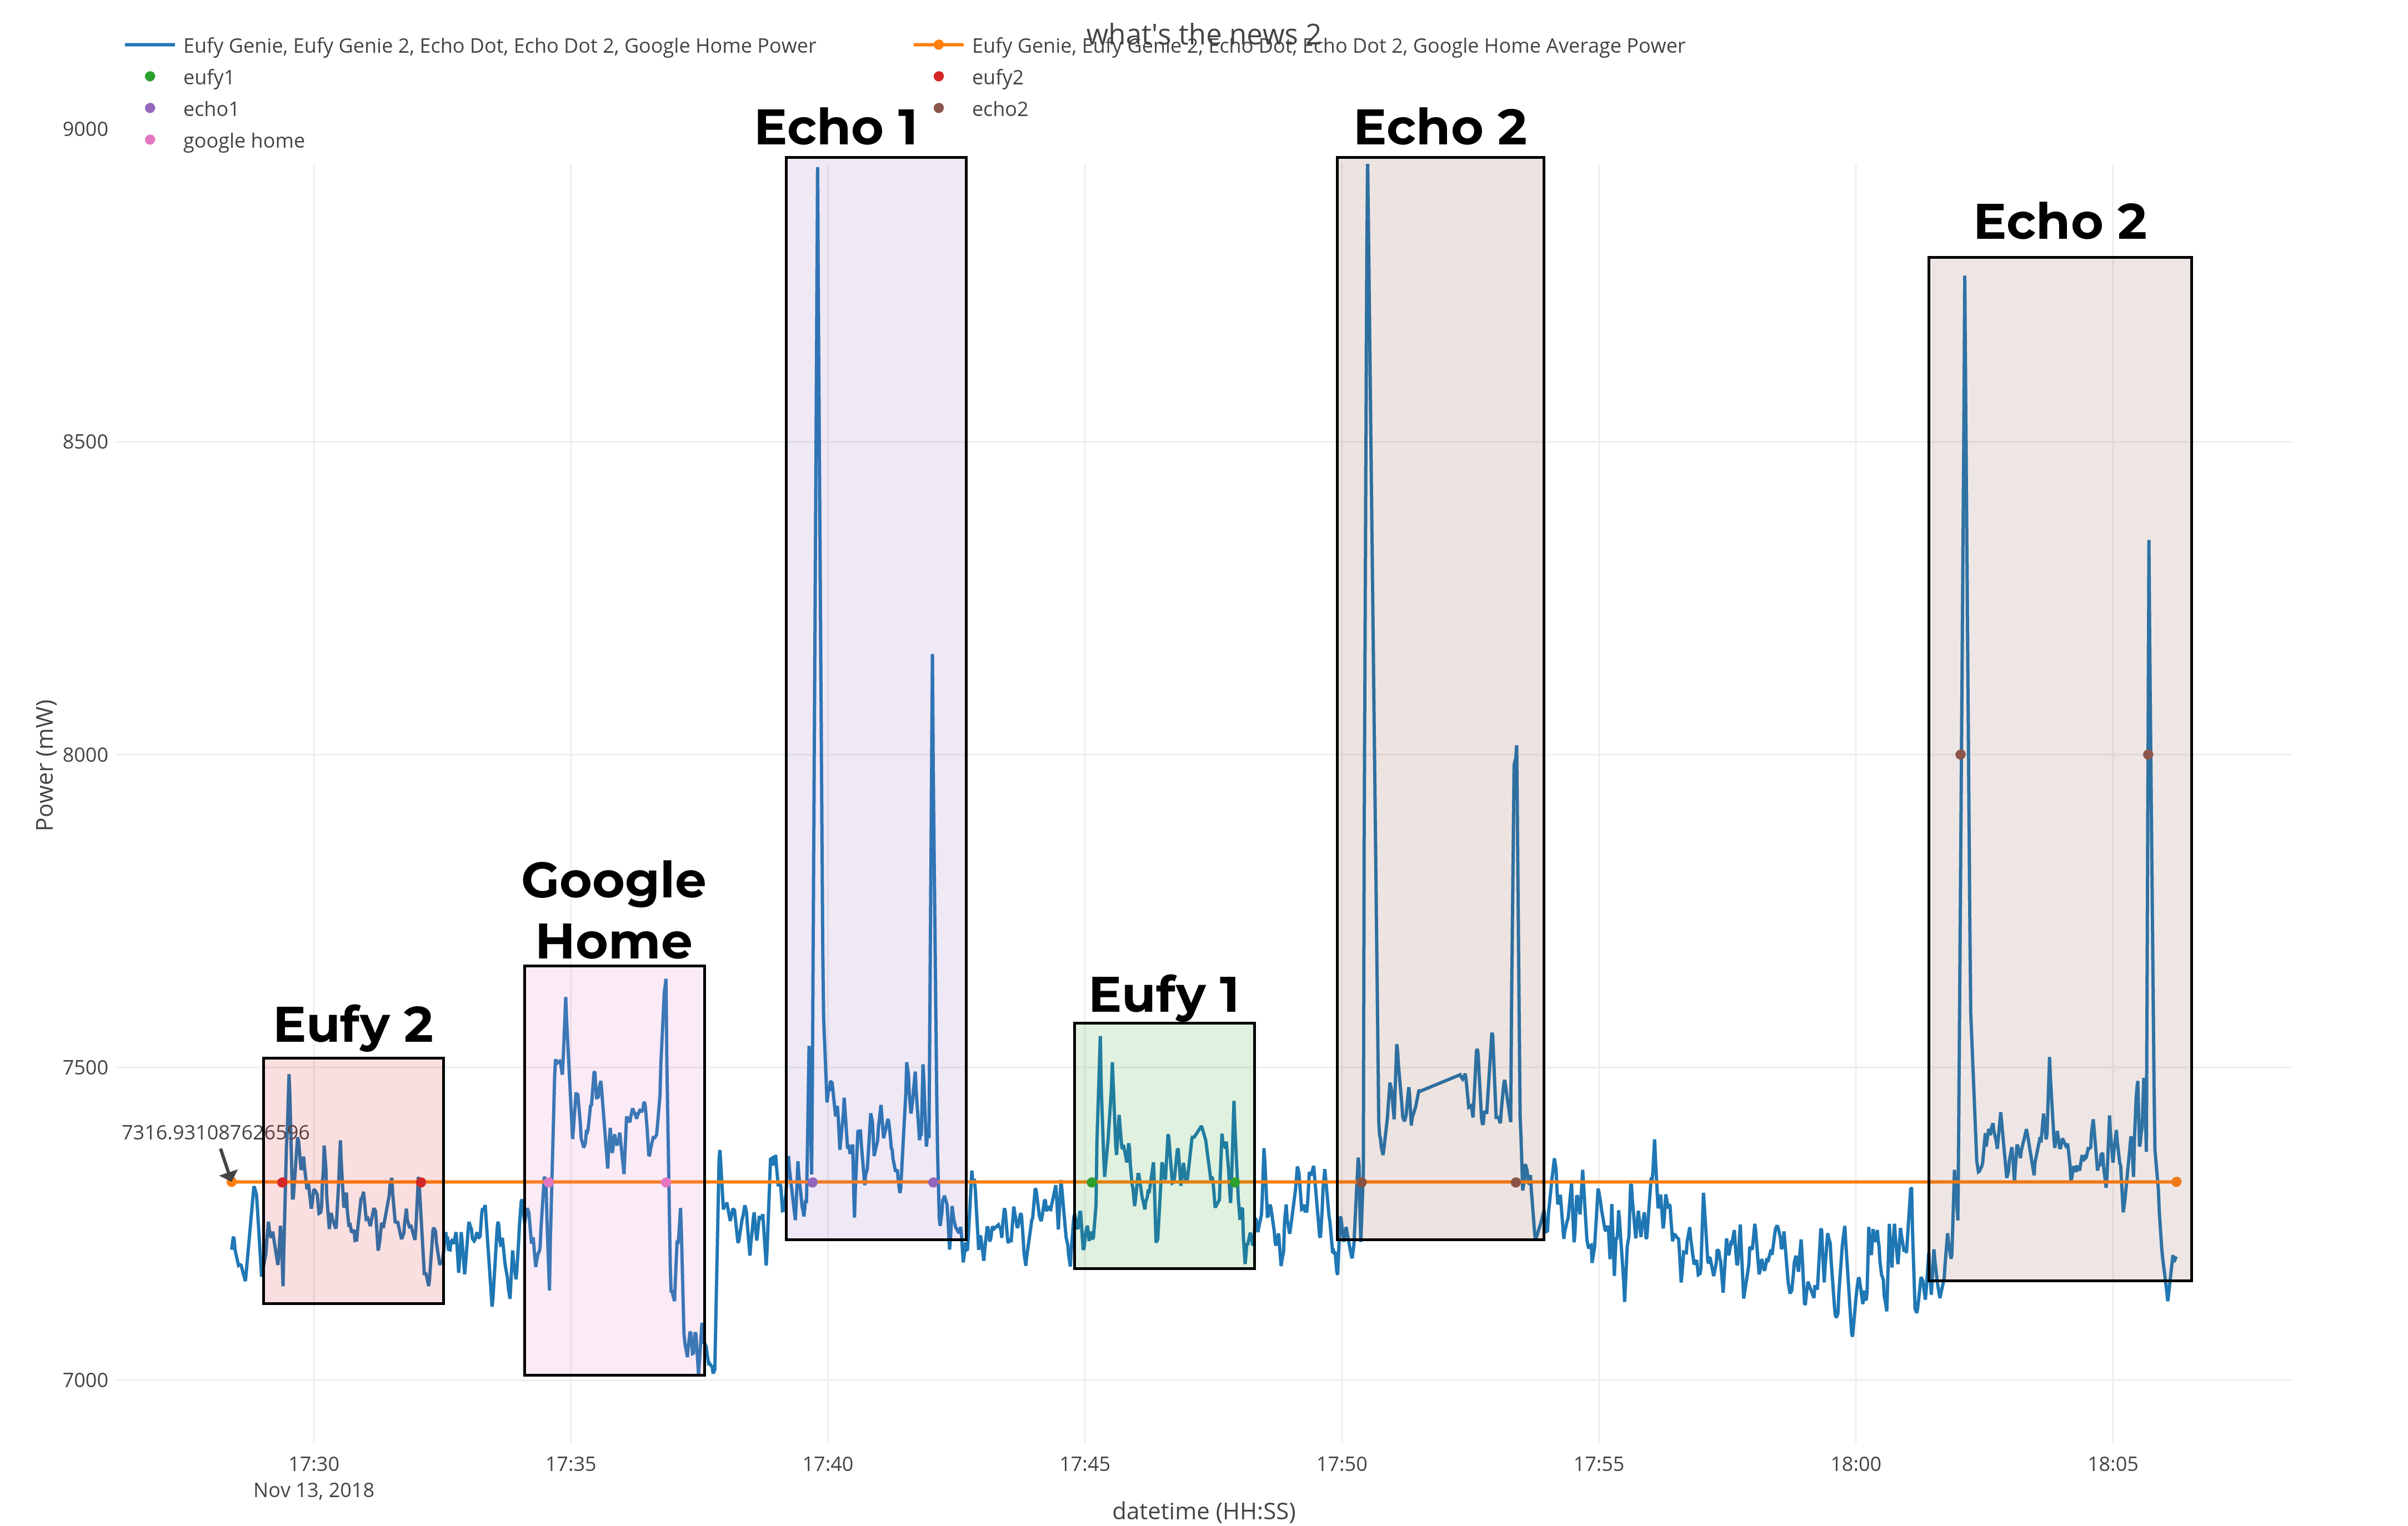
\includegraphics[width=1\textwidth]{figures/mixedNewsSum.png}
  \caption{5 Smart Speakers Power Summed Up. Queried each device for the
  news.}
  \label{fig:mixedNewsSum}
\end{figure}

The next graph, \ref{fig:bestBballSum}, shows the smart speakers when asked for the best basketball player. The annotation scheme is the same as before. Each smart speaker is queried for the best basketball player in consecutive order four times. Similar to before, the Eufy has a power spike of 420 mW peak to peak, the Google Home has a power Spike of 720 mW, and the Echo Dot has a power spike of 2180 mW.

When looking at graph \ref{fig:bestBballSum}, there is a power spike that is unaccounted for in correspondence to the event log at 18:12. We made a query, invoking all other power spikes but we did not do anything for the power spike at 18:12 that is higher than the other Eufy power spikes shown in first half of figure \ref{fig:bestBballSum} up to 18:24.

To figure what the power spike at 18:12 is, we separated the graphs into individual power traces as shown in figure \ref{fig:bestBballSeperate}. From this graph, the power spike at 18:12 is attributed to the Echo Dot 2 because it is the only trace with a spike occuring. We then looked at the individual network usage for each of these devices in this time frame as shown in figure \ref{fig:bestBballNetwork}. At 18:12, there is no significant network usage.

We had no conclusive evidence to decide what the power spike means. But in speculation, because there is no network usage during this time, we do not think the Echo Dot was doing anything data recording, listening, or was activated. We believe that the computer was covering the Echo Dot, but is briefly moved, exposing the Echo Dot to more light, thus causing the LEDs to brighten.

\begin{figure}[H]
  \centering
  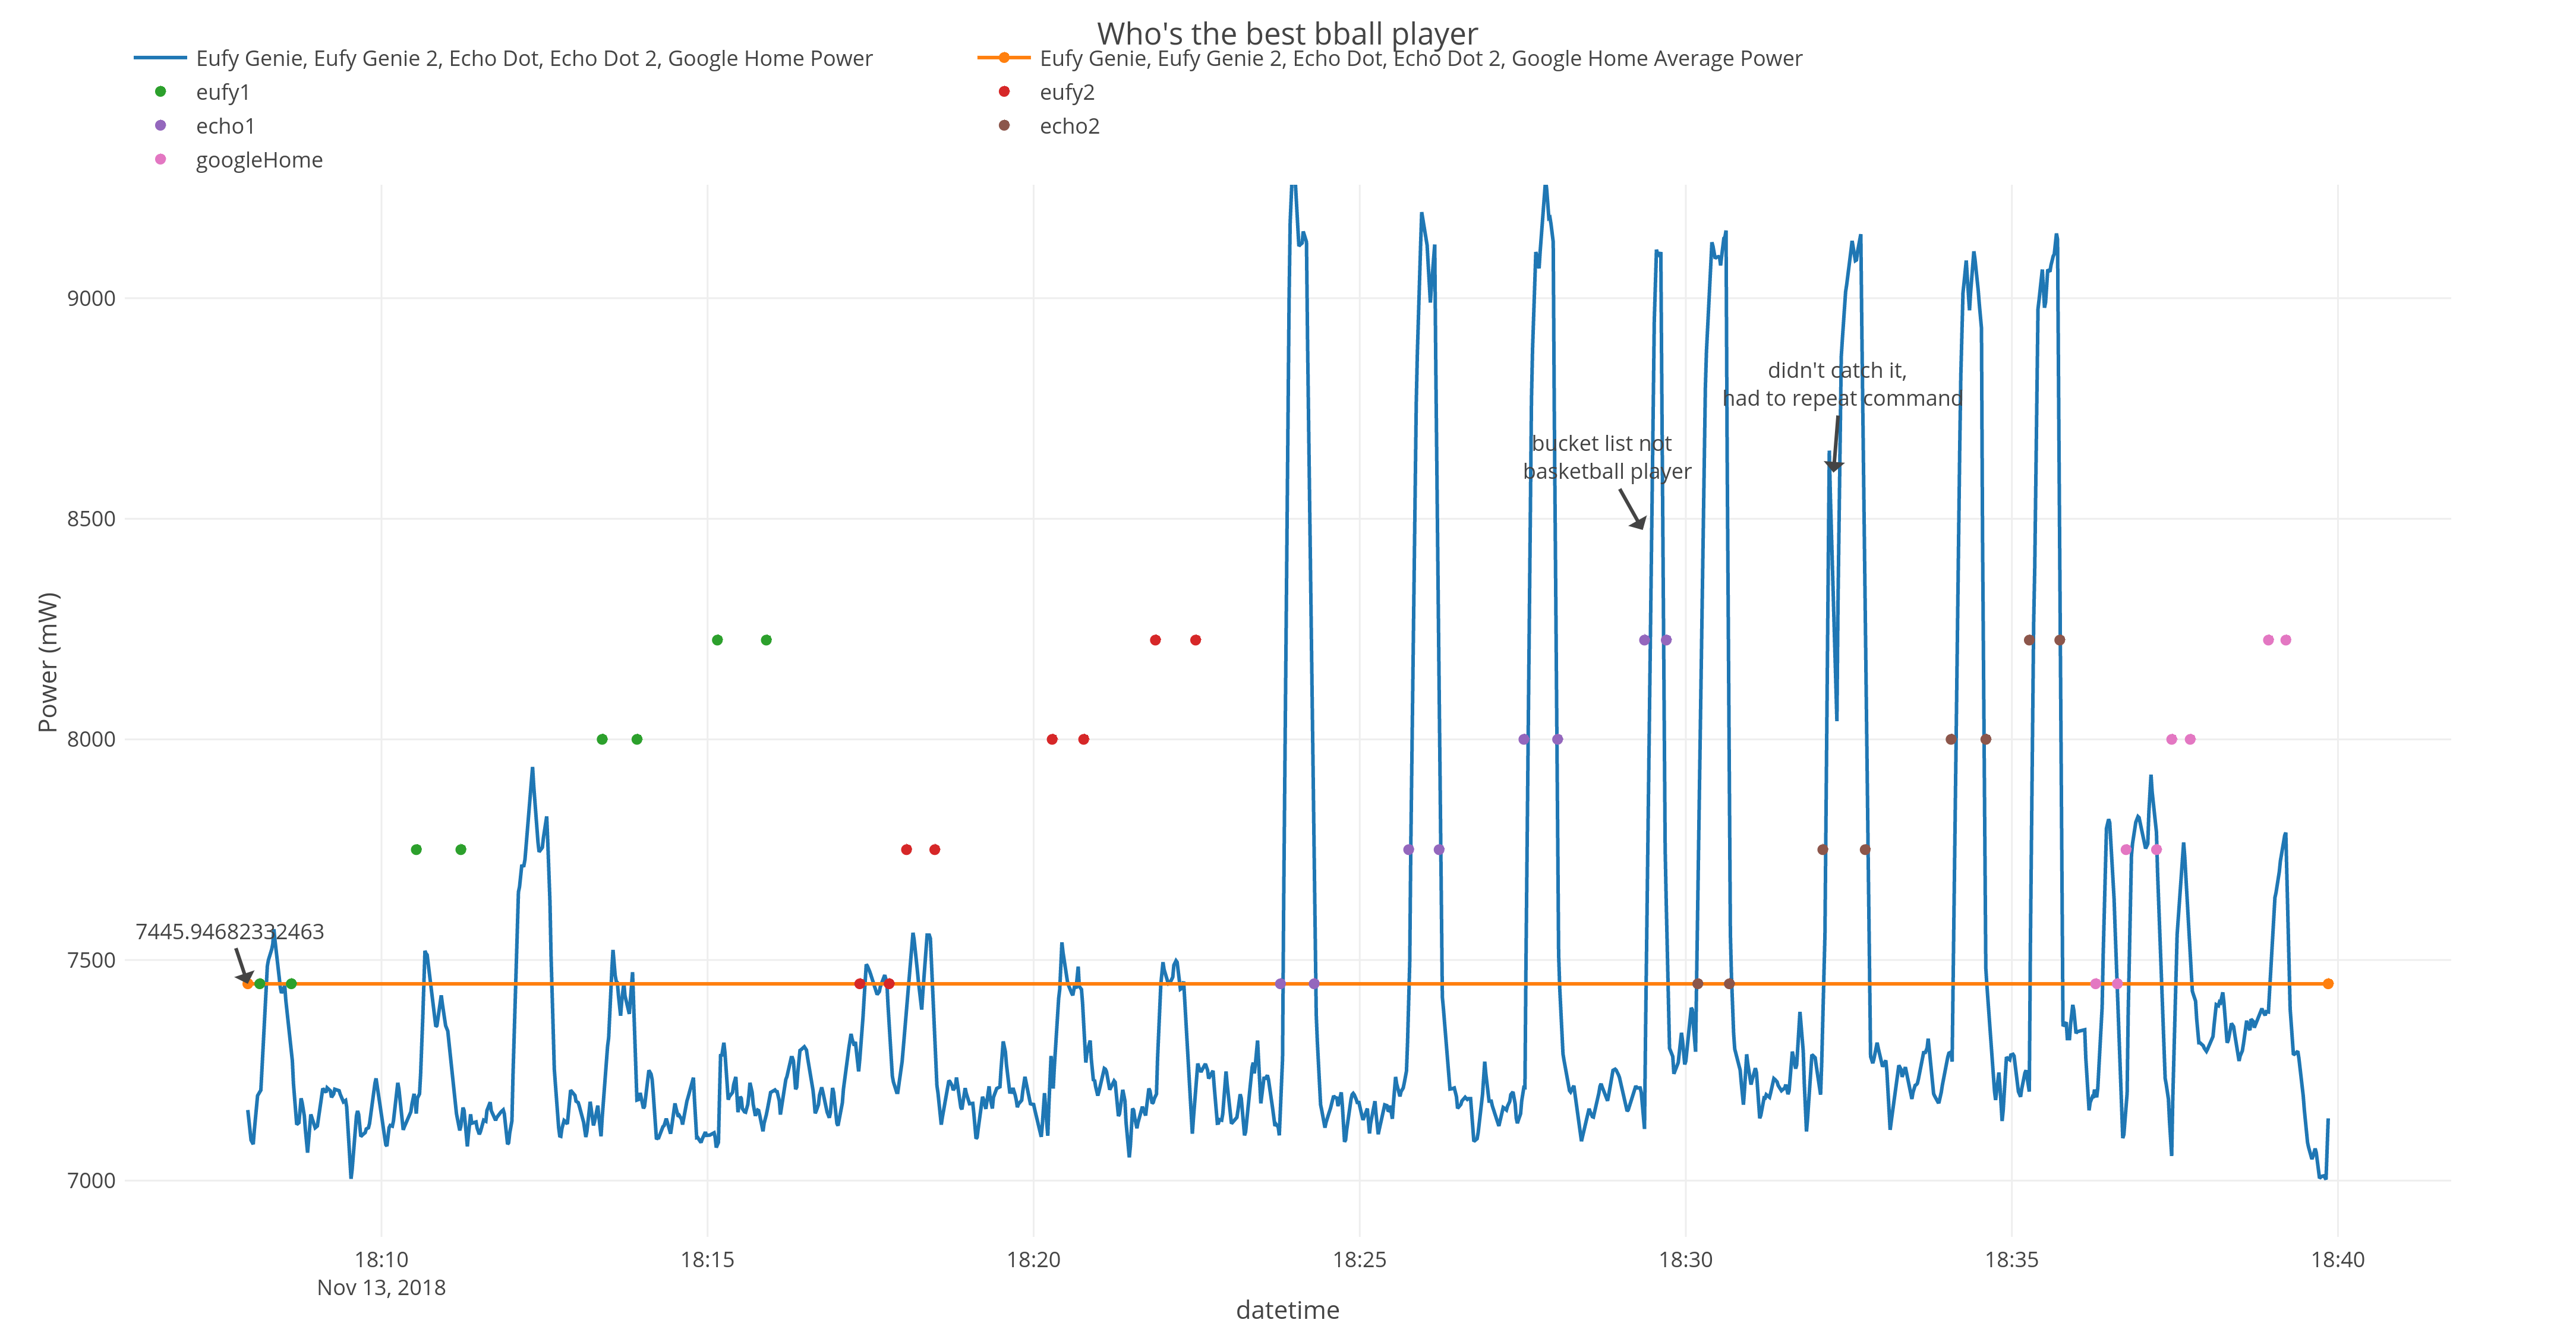
\includegraphics[width=1\textwidth]{figures/bestBballSum.png}
  \caption{5 Smart Speakers Power Summed Up. Queried each device for the
  best basketball player.}
  \label{fig:bestBballSum}
\end{figure}

\begin{figure}[H]
  \centering
  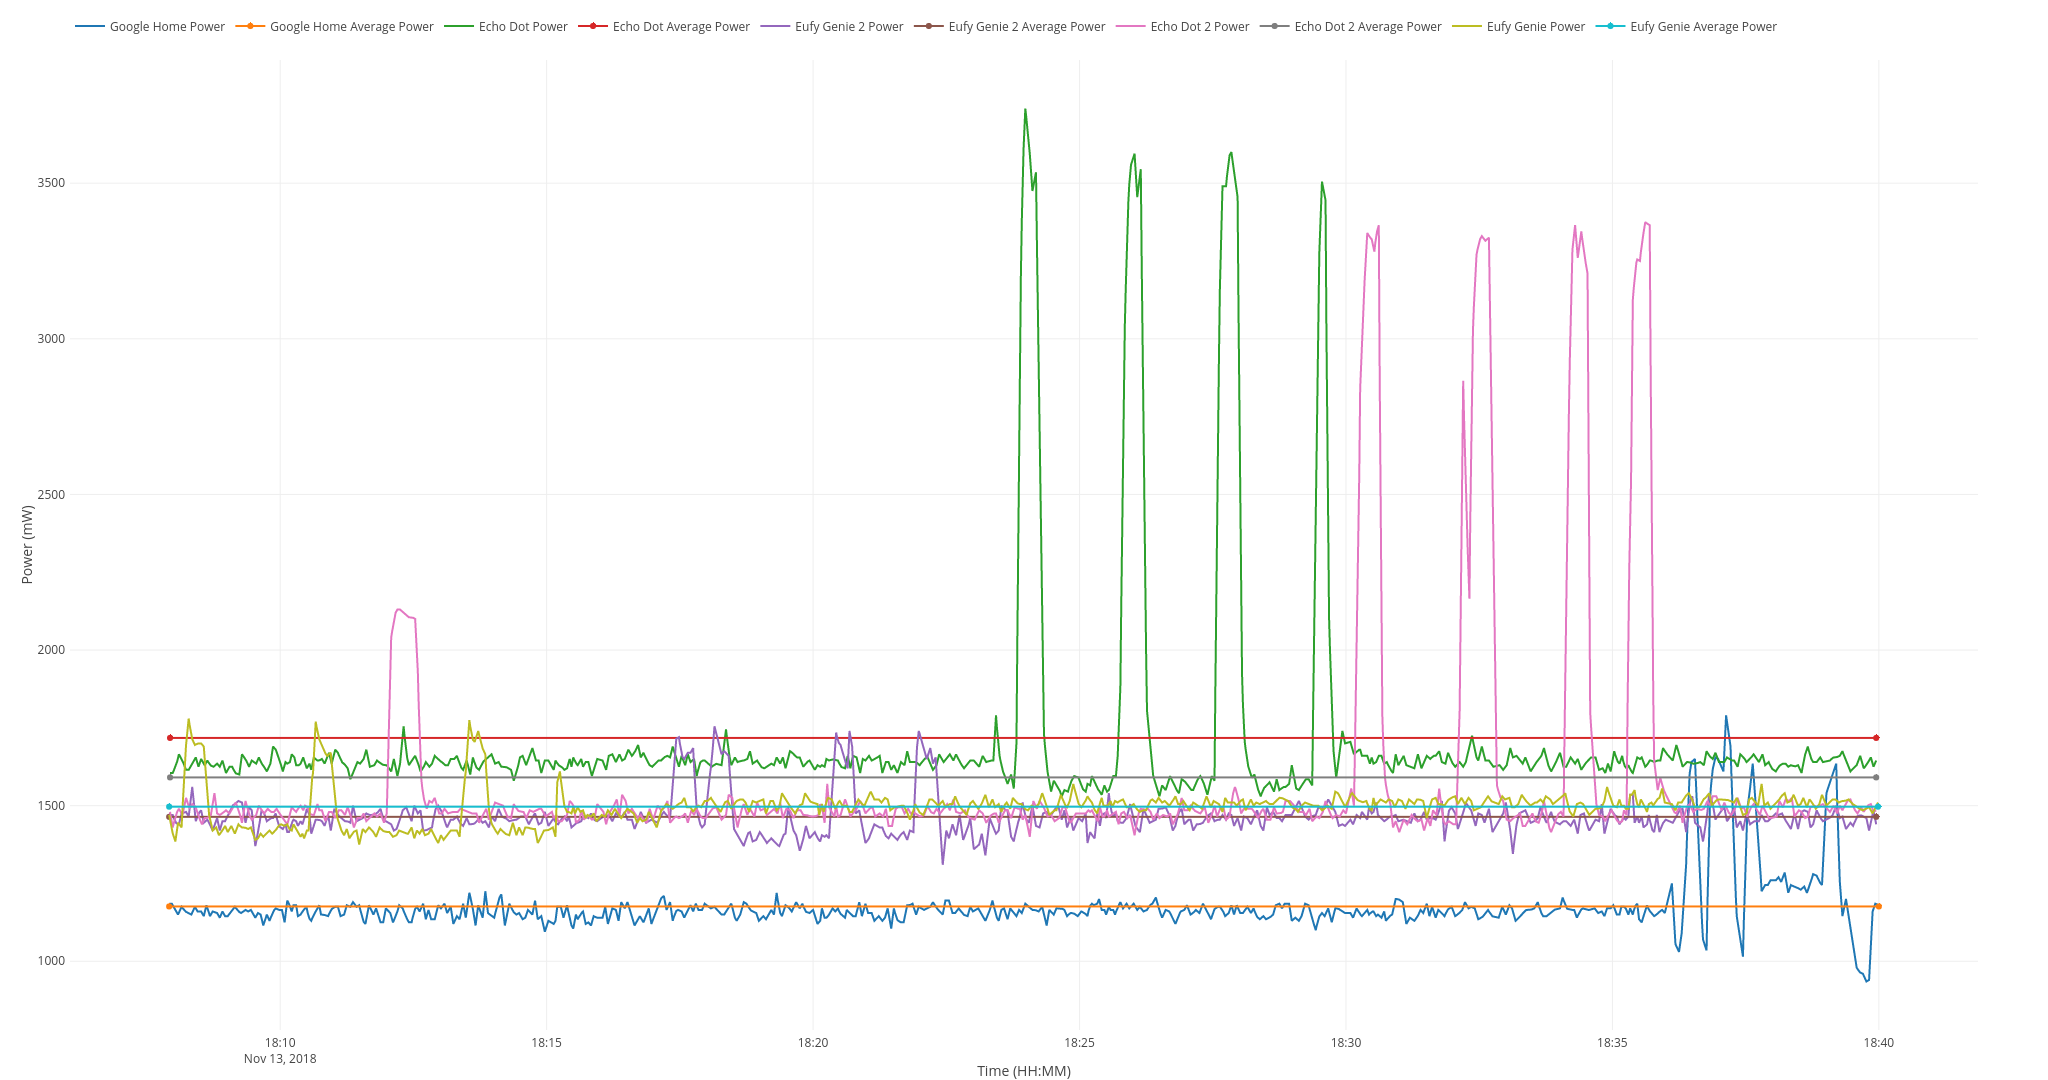
\includegraphics[width=1\textwidth]{figures/bestBballSeperate.png}
  \caption{5 Smart Speakers Power Usage over time. Queried each device for the
  best basketball player.}
  \label{fig:bestBballSeperate}
\end{figure}

\begin{figure}[H]
  \centering
  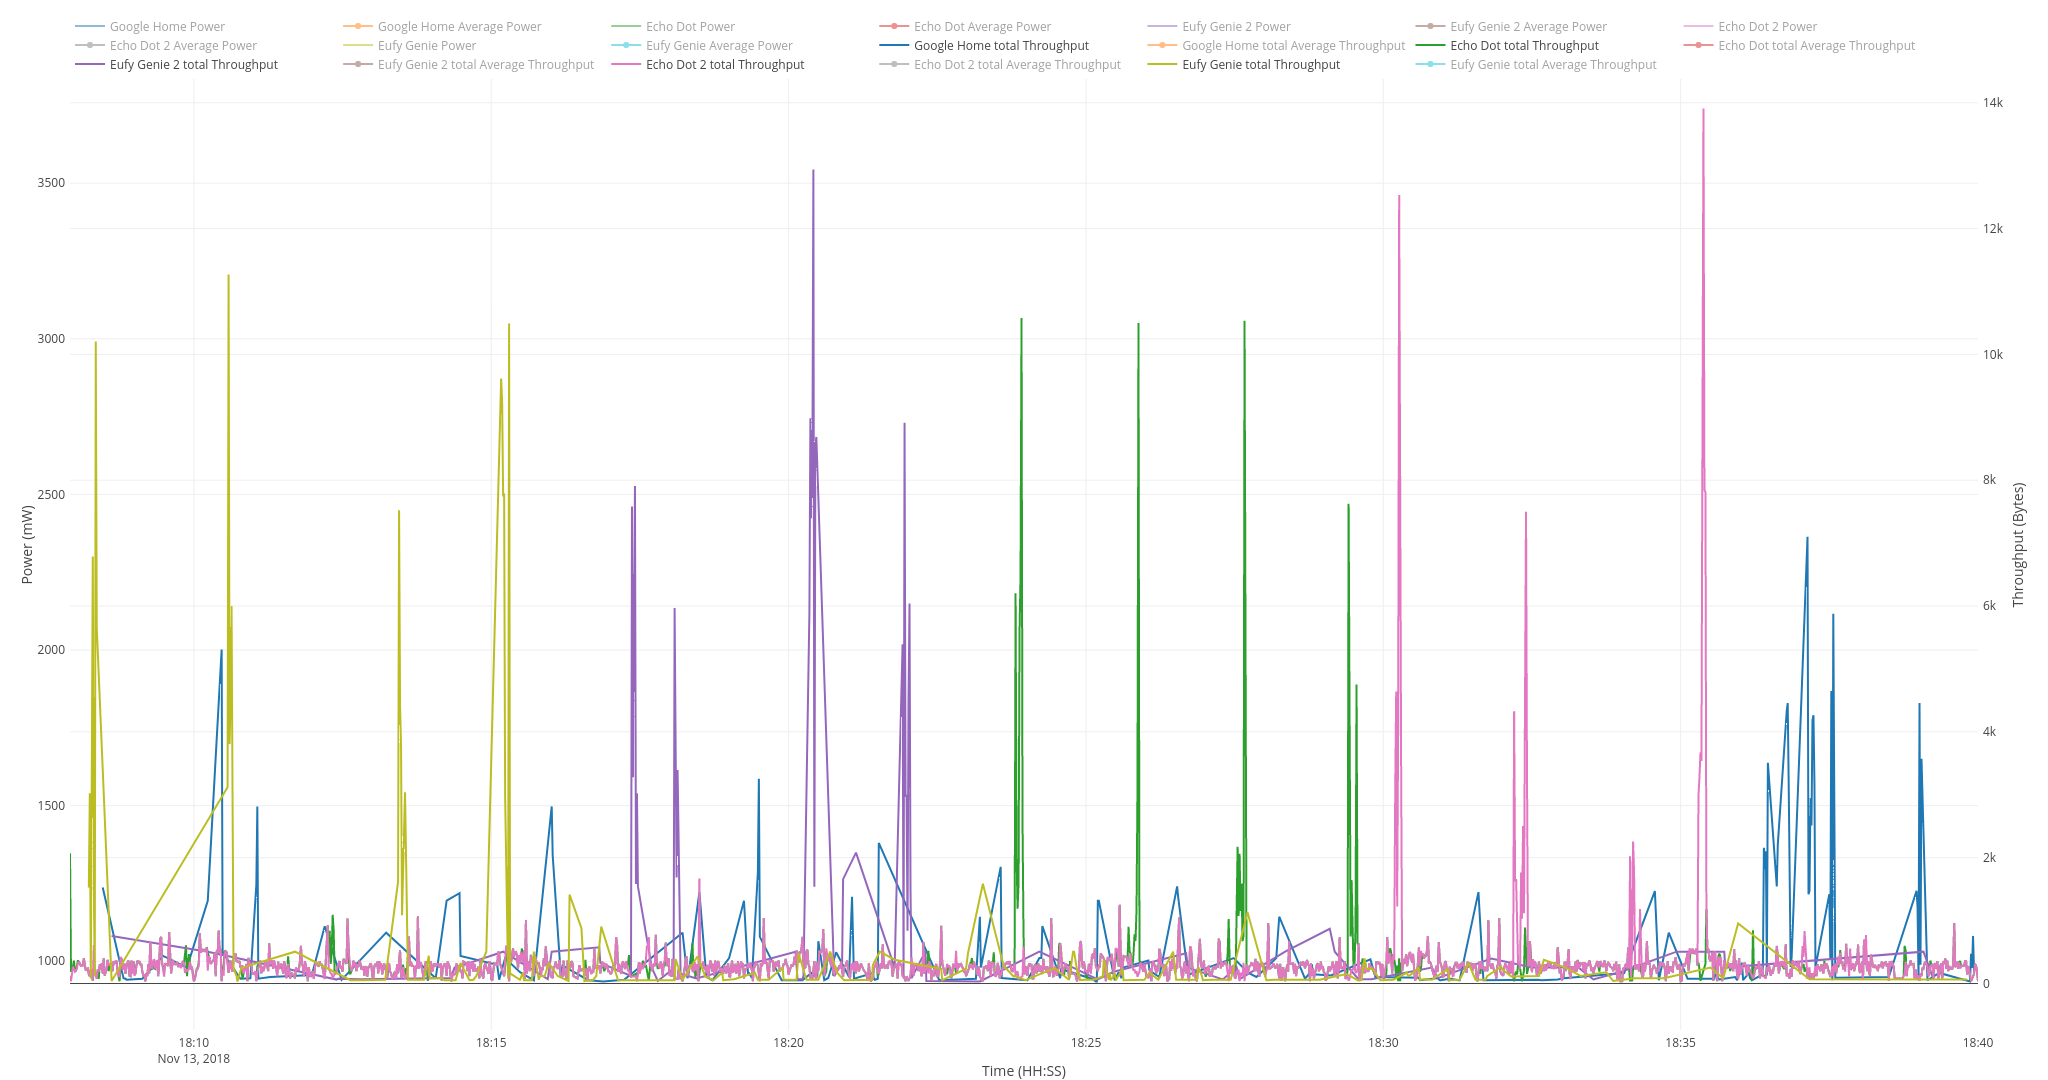
\includegraphics[width=1\textwidth]{figures/bestBballNetwork.png}
  \caption{5 Smart Speakers Network throughput over time. Queried each device for the best basketball player.}
  \label{fig:bestBballNetwork}
\end{figure}

The power spike information for each query type (``what's the weather'' ``what's the news'', ``who's the best basketball player'') is shown below in figure \ref{fig:spikeVoltages}. From figures \ref{fig:weatherSum}, \ref{fig:mixedNewsSum}, and \ref{fig:bestBballSum} there is always a characteristic power spike that occurs at the beginning of a command for each device. This bar graph also includes the total average spike height for each command for all three of these commands. The black line at the top of each bar shows the standard deviation. Averaging peak to peak voltage spikes for each device shows the Eufy Genie with a 390 mW spike with 36.1 mW standard deviation, the Google Home with a 606.7 mW spike with 110 mW standard deviation, the Echo Dot with a 2026.7 mW spike with 149.89 mW standard deviation.

From figure \ref{fig:spikeVoltages}, we can determine what device model is being used if it is within those thresholds. The models with multiple units are consistent with each other. From this, we conclude it is possible to determine a device model from visual examination of its power usage. This is our first step to testing our hypotheses that it is possible to see what devices are in use from analysis of someone's power line.

\begin{figure}[H]
  \centering
  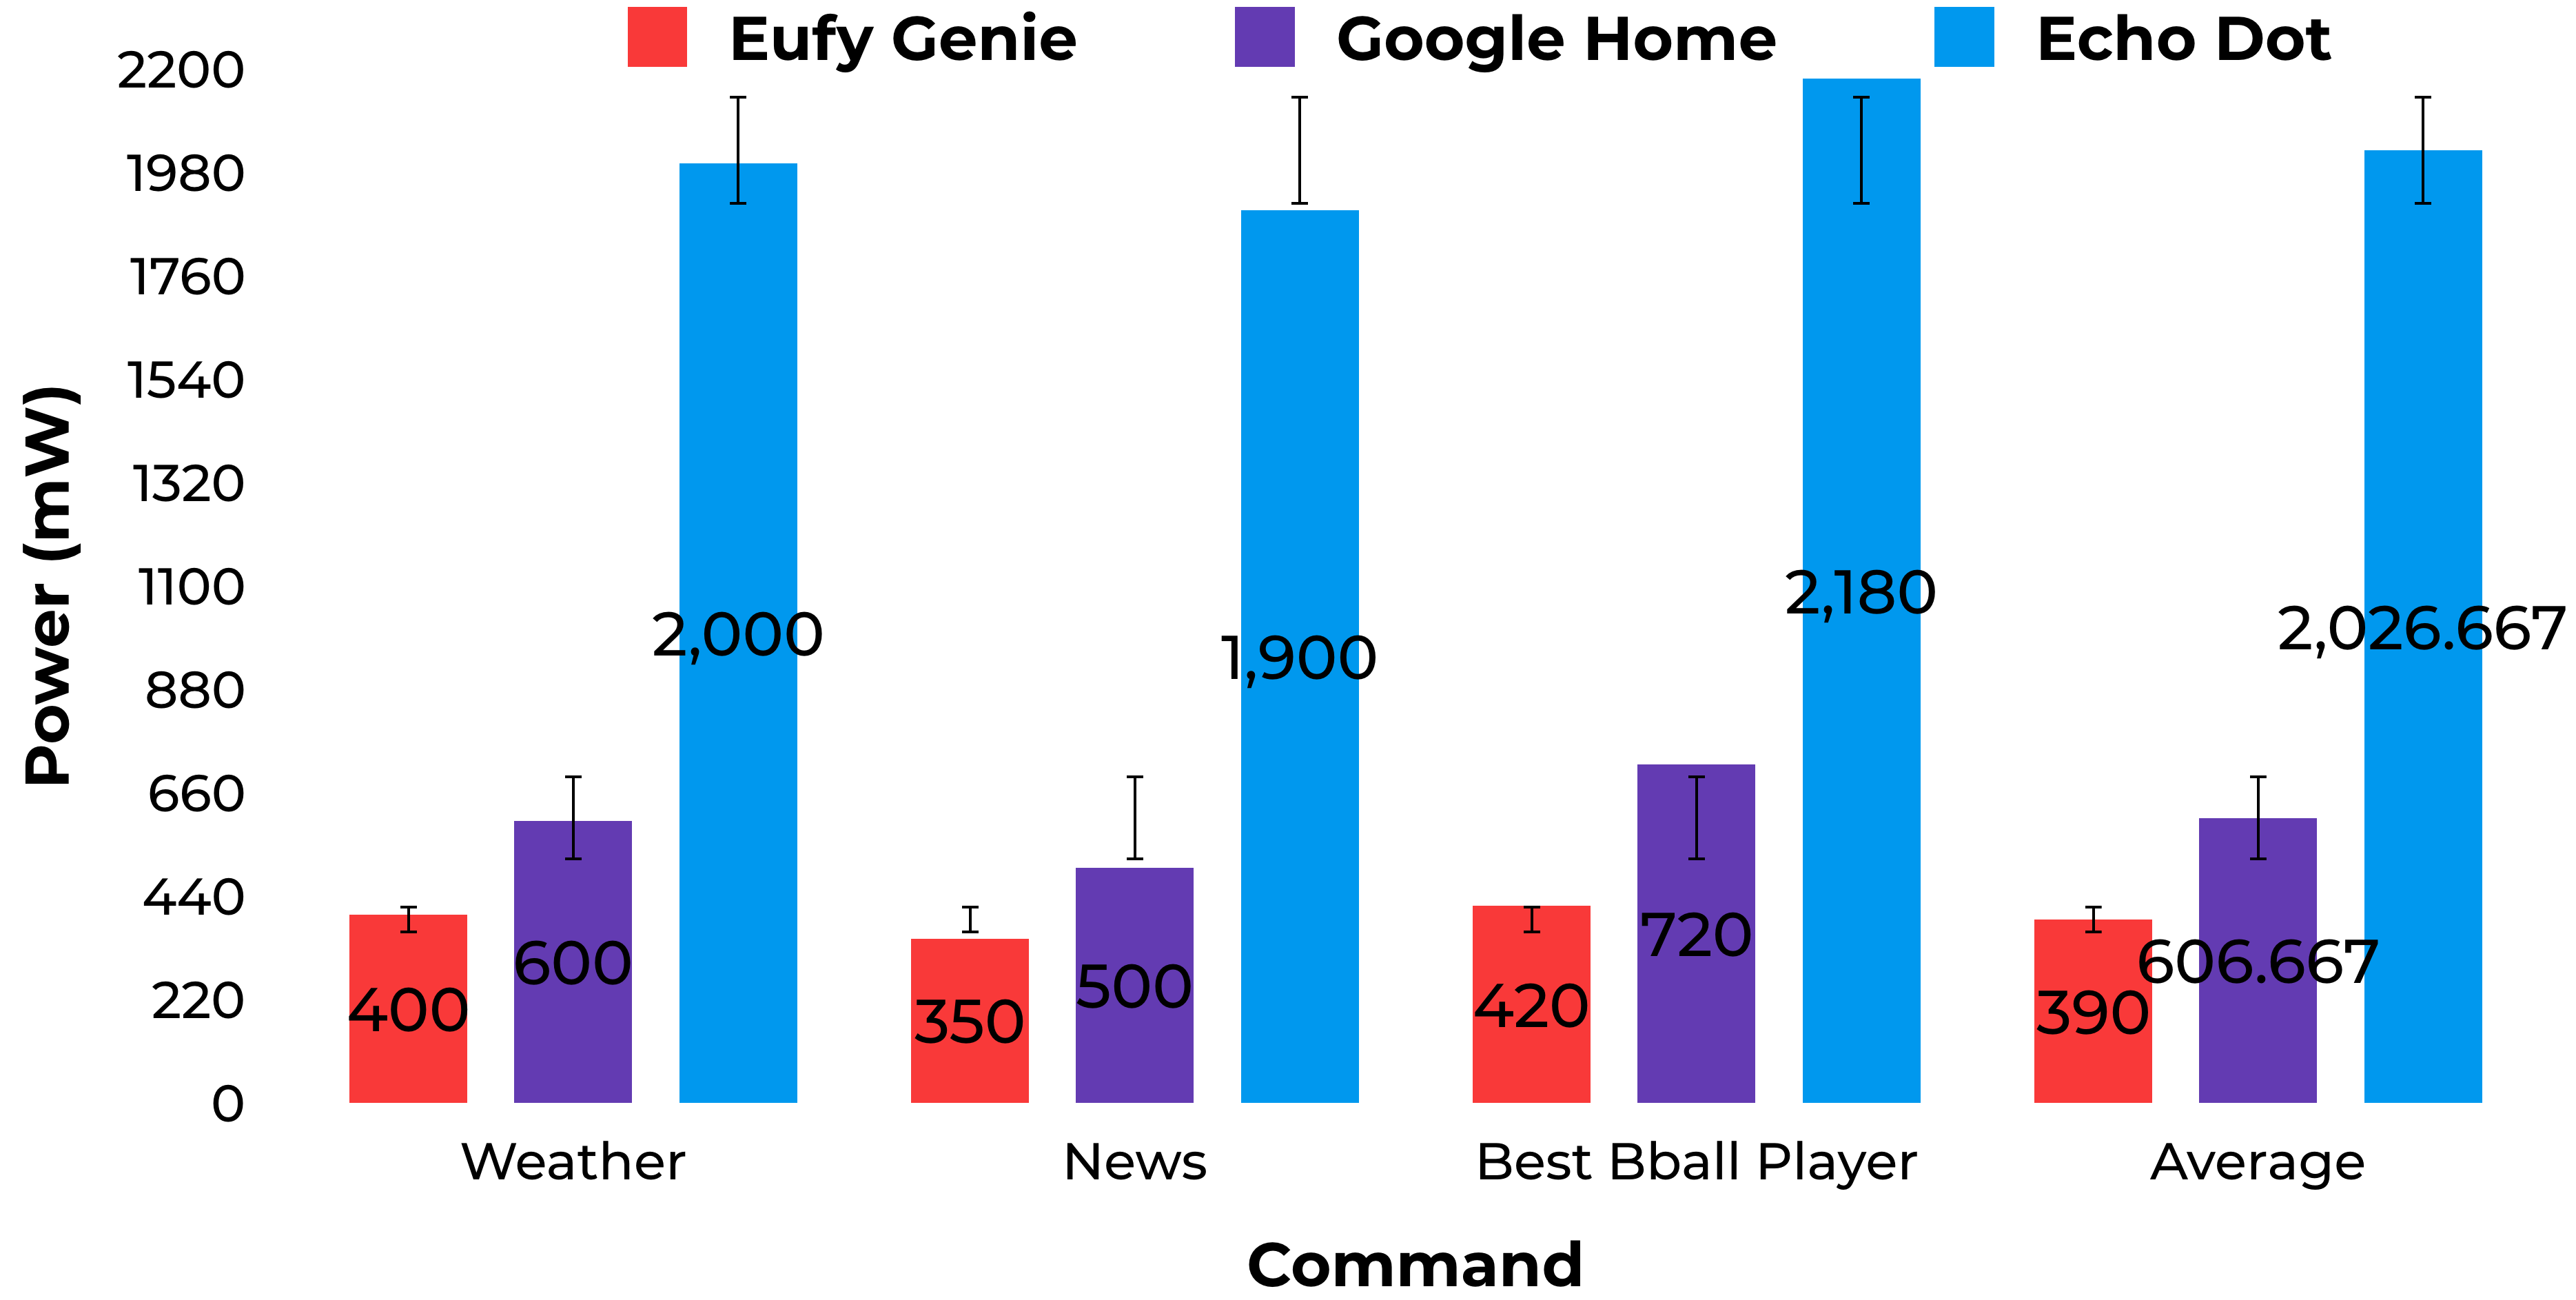
\includegraphics[width=1\textwidth]{figures/spikeVoltages.png}
  \caption{Spike summary of for each query.}
  \label{fig:spikeVoltages}
\end{figure}

But in a real house, there are more than just 5 smart speakers on a power line. The next step is to add noise from high power devices to see if it is still possible to visually determine the device in use from power spikes \ref{sumPowerGraphWithNoise}.

\section{Summed Power Graph With Noise}
\label{sumPowerGraphWithNoise}
In this section, we introduce noise into the system so that we can determine if the power spike from each smart speaker is still discernible within a summed power graph when we add high power devices.

In each subsection, there are three traces. The first trace (blue trace) is the summed power usage of our five smart speakers (2 Echo Dots, 2 Eufy Genies, 1 Google Home) when asked for the best basketball player 4 times. This is the same trace as shown in \ref{fig:bestBballSum}. is the power usage over time for a high power device. The second trace (purple trace) is the power usage of a high power device. This trace is the added noise. It maps to various devices as we switch them out. The third trace (red trace) is the sum of both trace 1 and 2. It is the power usage of the smart speakers in the blue trace with the noise from the device in the purple trace.

There x-axis is the time elapsed in seconds. There is no time vecause the smart speaker trace was taken at a seperate time from when the noise trace was taken. The y-axis is the power used by each device over time.

Below, in figure \ref{fig:fanIdleSeperate}, is an example of the traces used seperately. Taking the blue trace (smart speaker power usage) and the purple trace (noise introducing device) the summed up graph will result in the red trace (total power usage). This is shown seperately at first, but will be summed together for the rest of the paper so that the scale of the noise can be understood.

\begin{figure}[H]
  \centering
  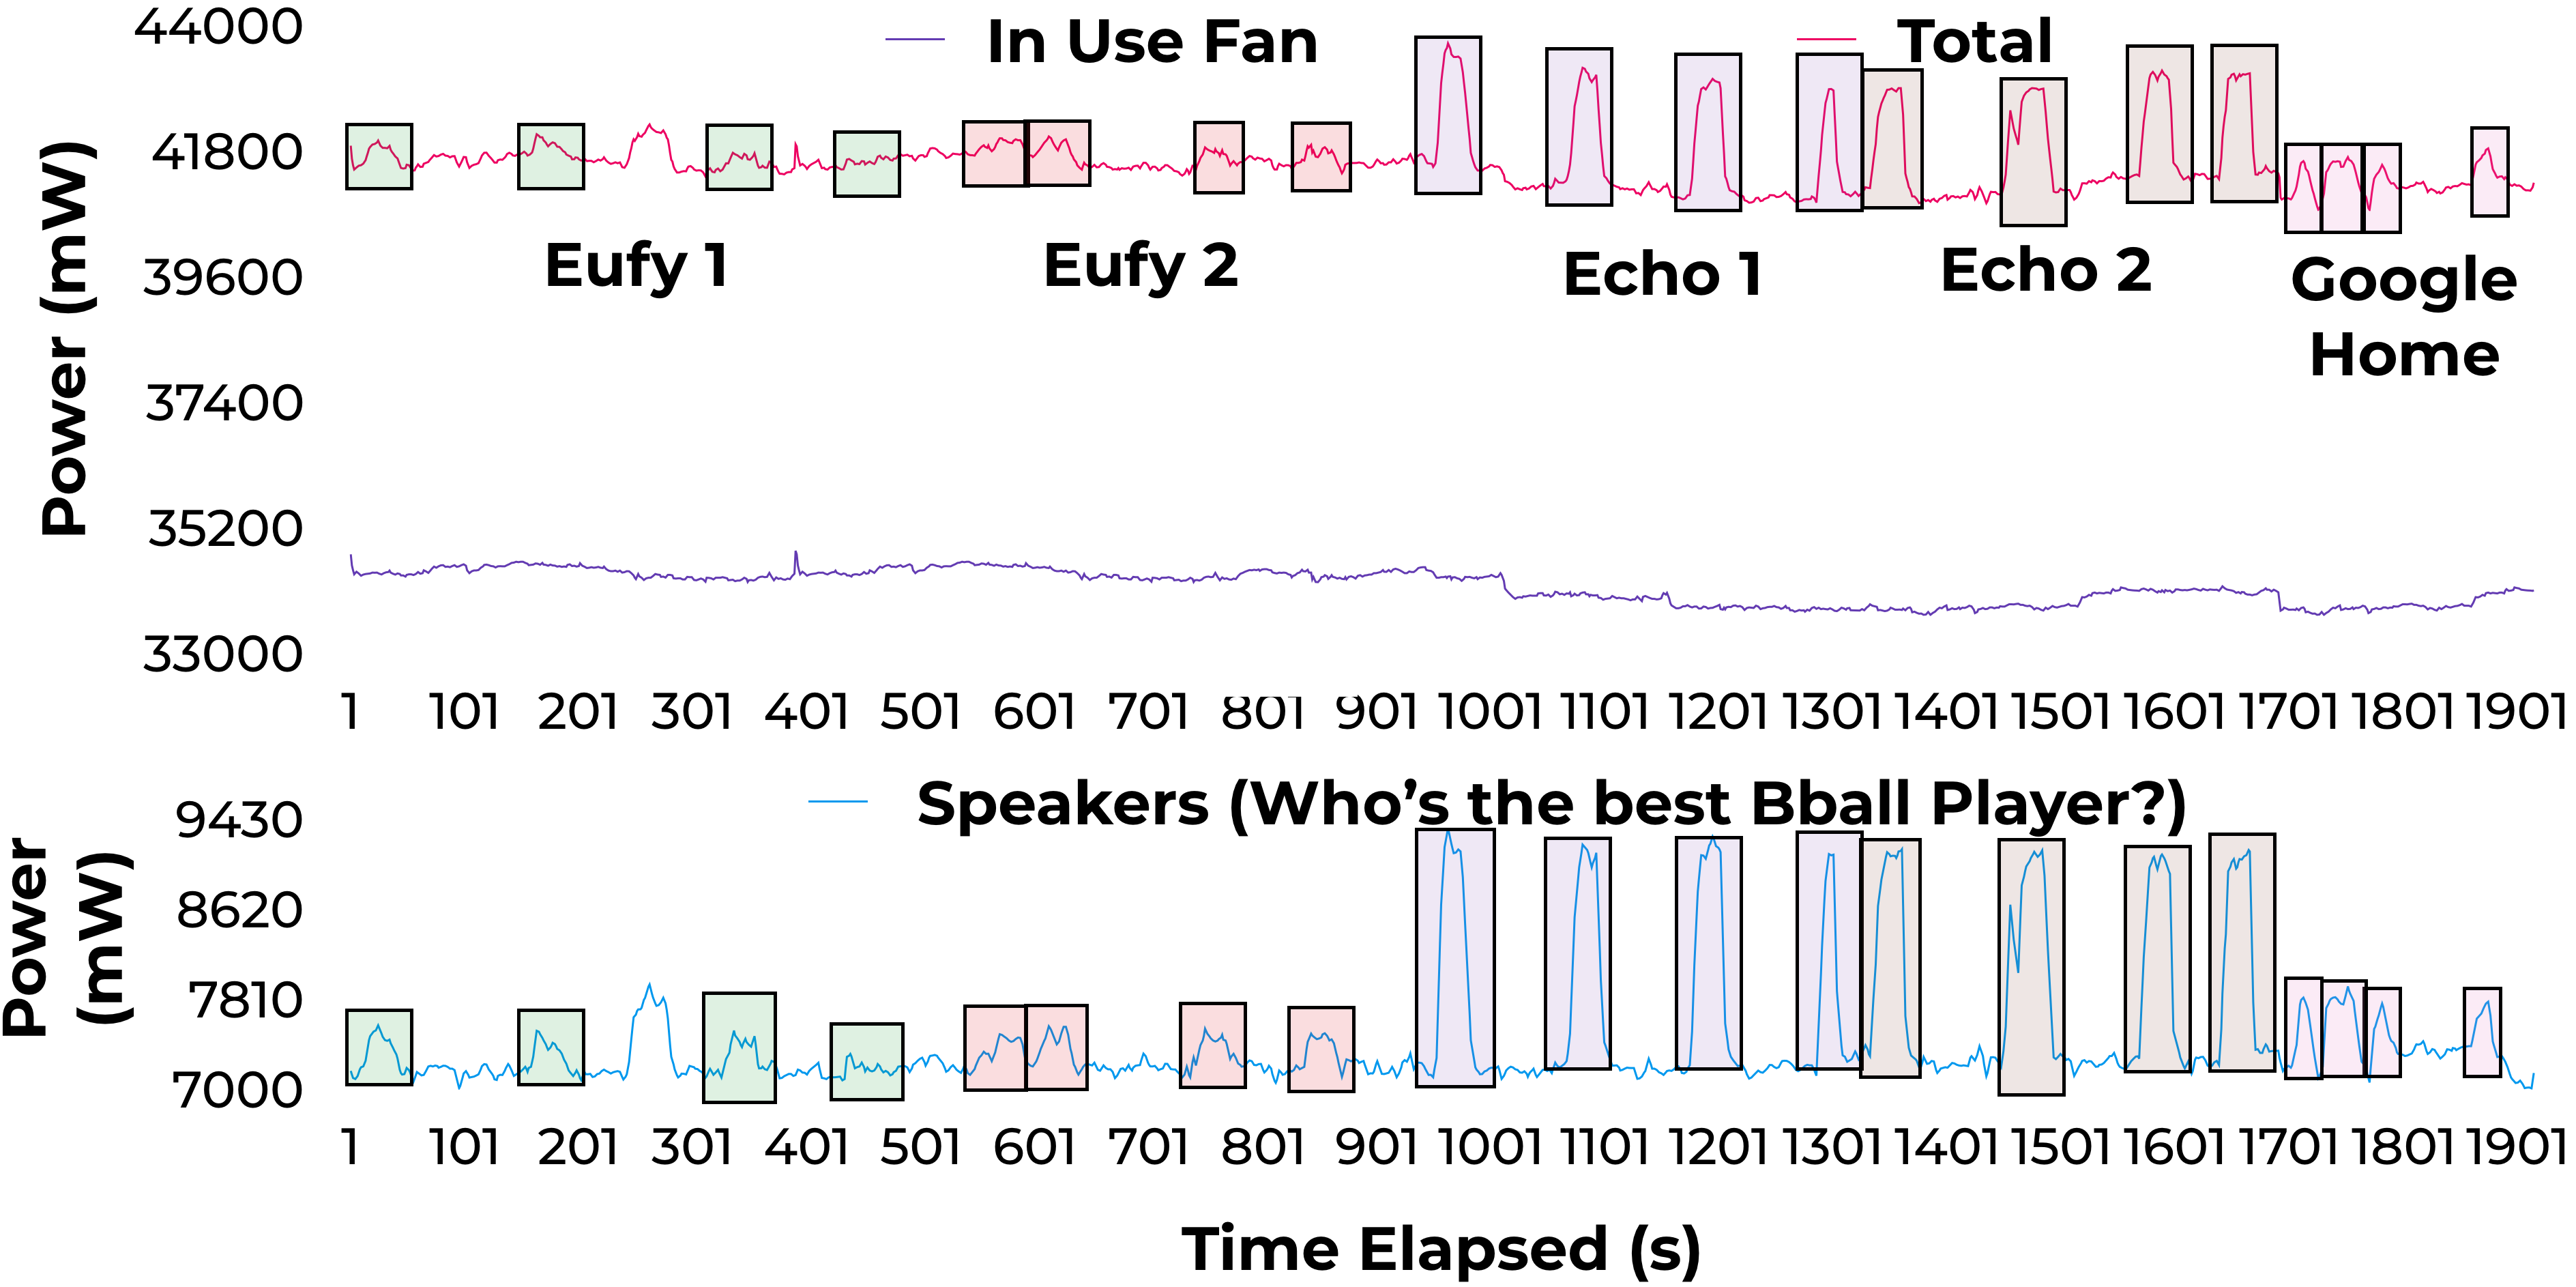
\includegraphics[width=1\textwidth]{figures/inUseFanNoiseSeperate.png}
  \caption{Idle Fan with figure \ref{fig:bestBballSum} trace shown seperately.}
  \label{fig:fanIdleSeperate}
\end{figure}

Below, we display the smart speaker trace with a PC (Intel NUC), fan, refrigerator, or microwave. Figures \ref{fig:fanIdleSeperate}, \ref{fig:fanIdle}, \ref{fig:uWaveIdle}, \ref{fig:fridgeIdle}, \ref{fig:nucIdle}, and \ref{fig:allIdleNoise} begin with noise from devices while idle or during steady power usage to set a baseline. Then figures \ref{fig:uWaveInUse}, \ref{fig:fridgeInUse}, and \ref{fig:nucInUse} show noise from devices while in use, introducing noise that make visual detection of smart speakers most difficult.

In figures \ref{fig:fanIdle}, \ref{fig:uWaveIdle}, \ref{fig:fridgeIdle}, and \ref{fig:nucIdle}, the power spikes from the smart speakers can still be seen. Visually, the Echo Dot power spike is clearly seen in red trace for each graph. The power spikes for the Google Home and Eufy Genie are less visible but can still be seen. Especially when zoomed in as shown in figure \ref{fig:allIdleNoise} where the smart speaker trace is removed.

\begin{figure}[H]
  \centering
  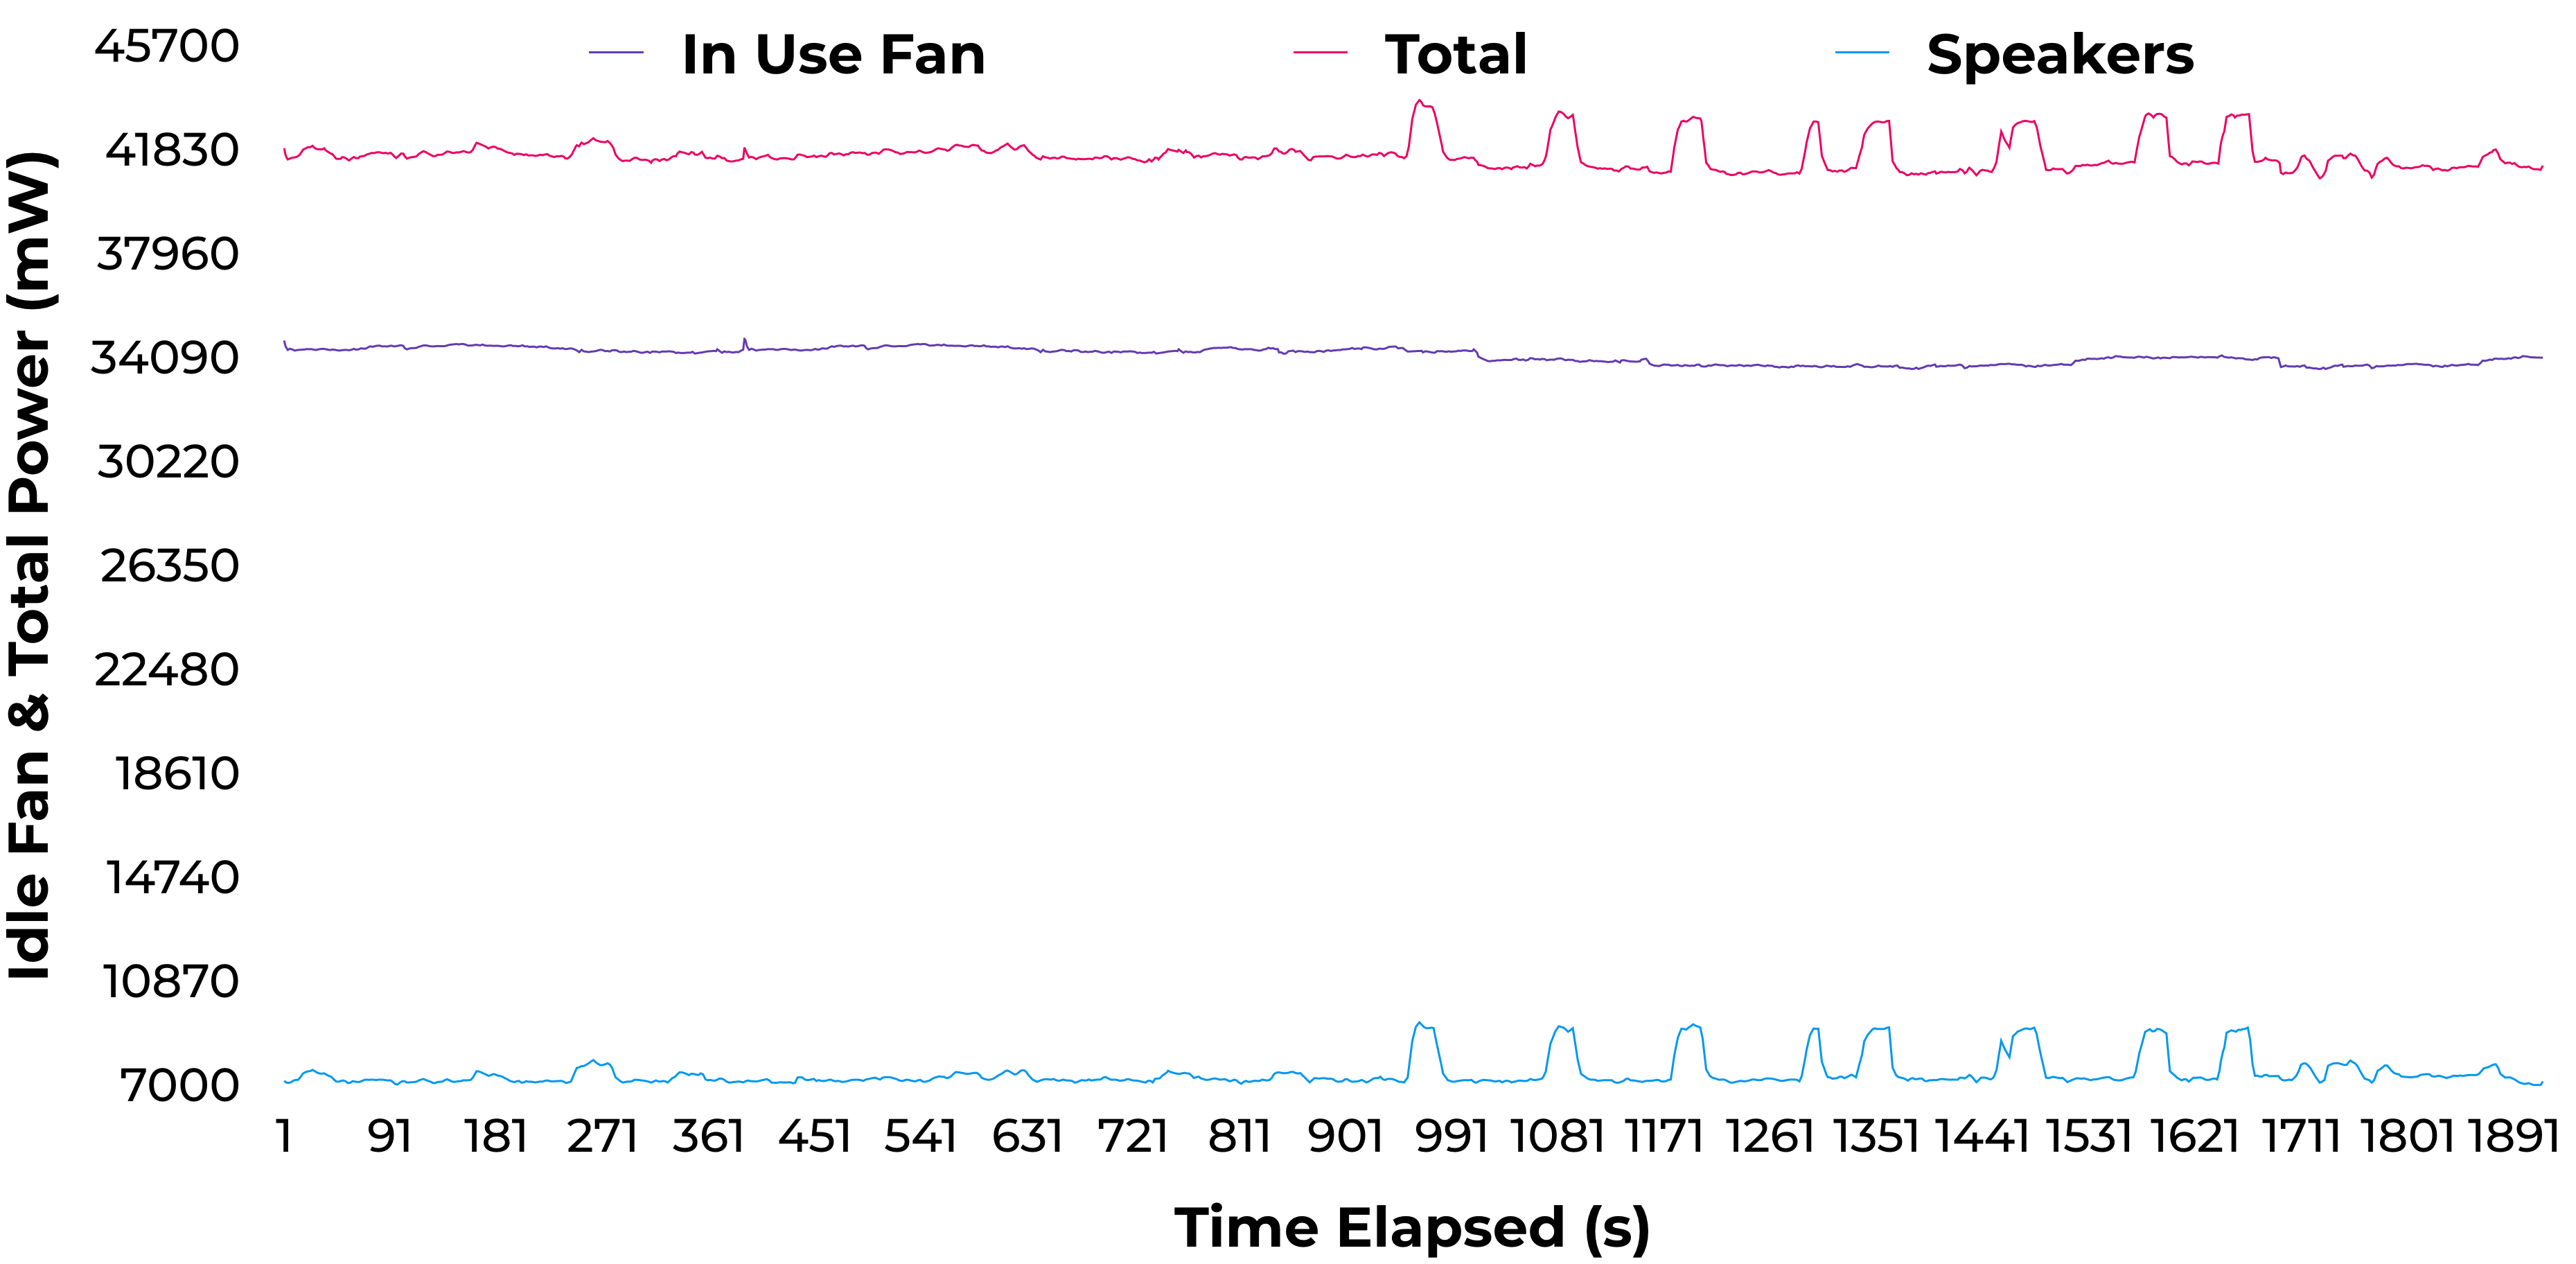
\includegraphics[width=1\textwidth]{figures/inUseFanNoise.png}
  \caption{Idle Fan with figure \ref{fig:bestBballSum} trace.}
  \label{fig:fanIdle}
\end{figure}

\begin{figure}[H]
  \centering
  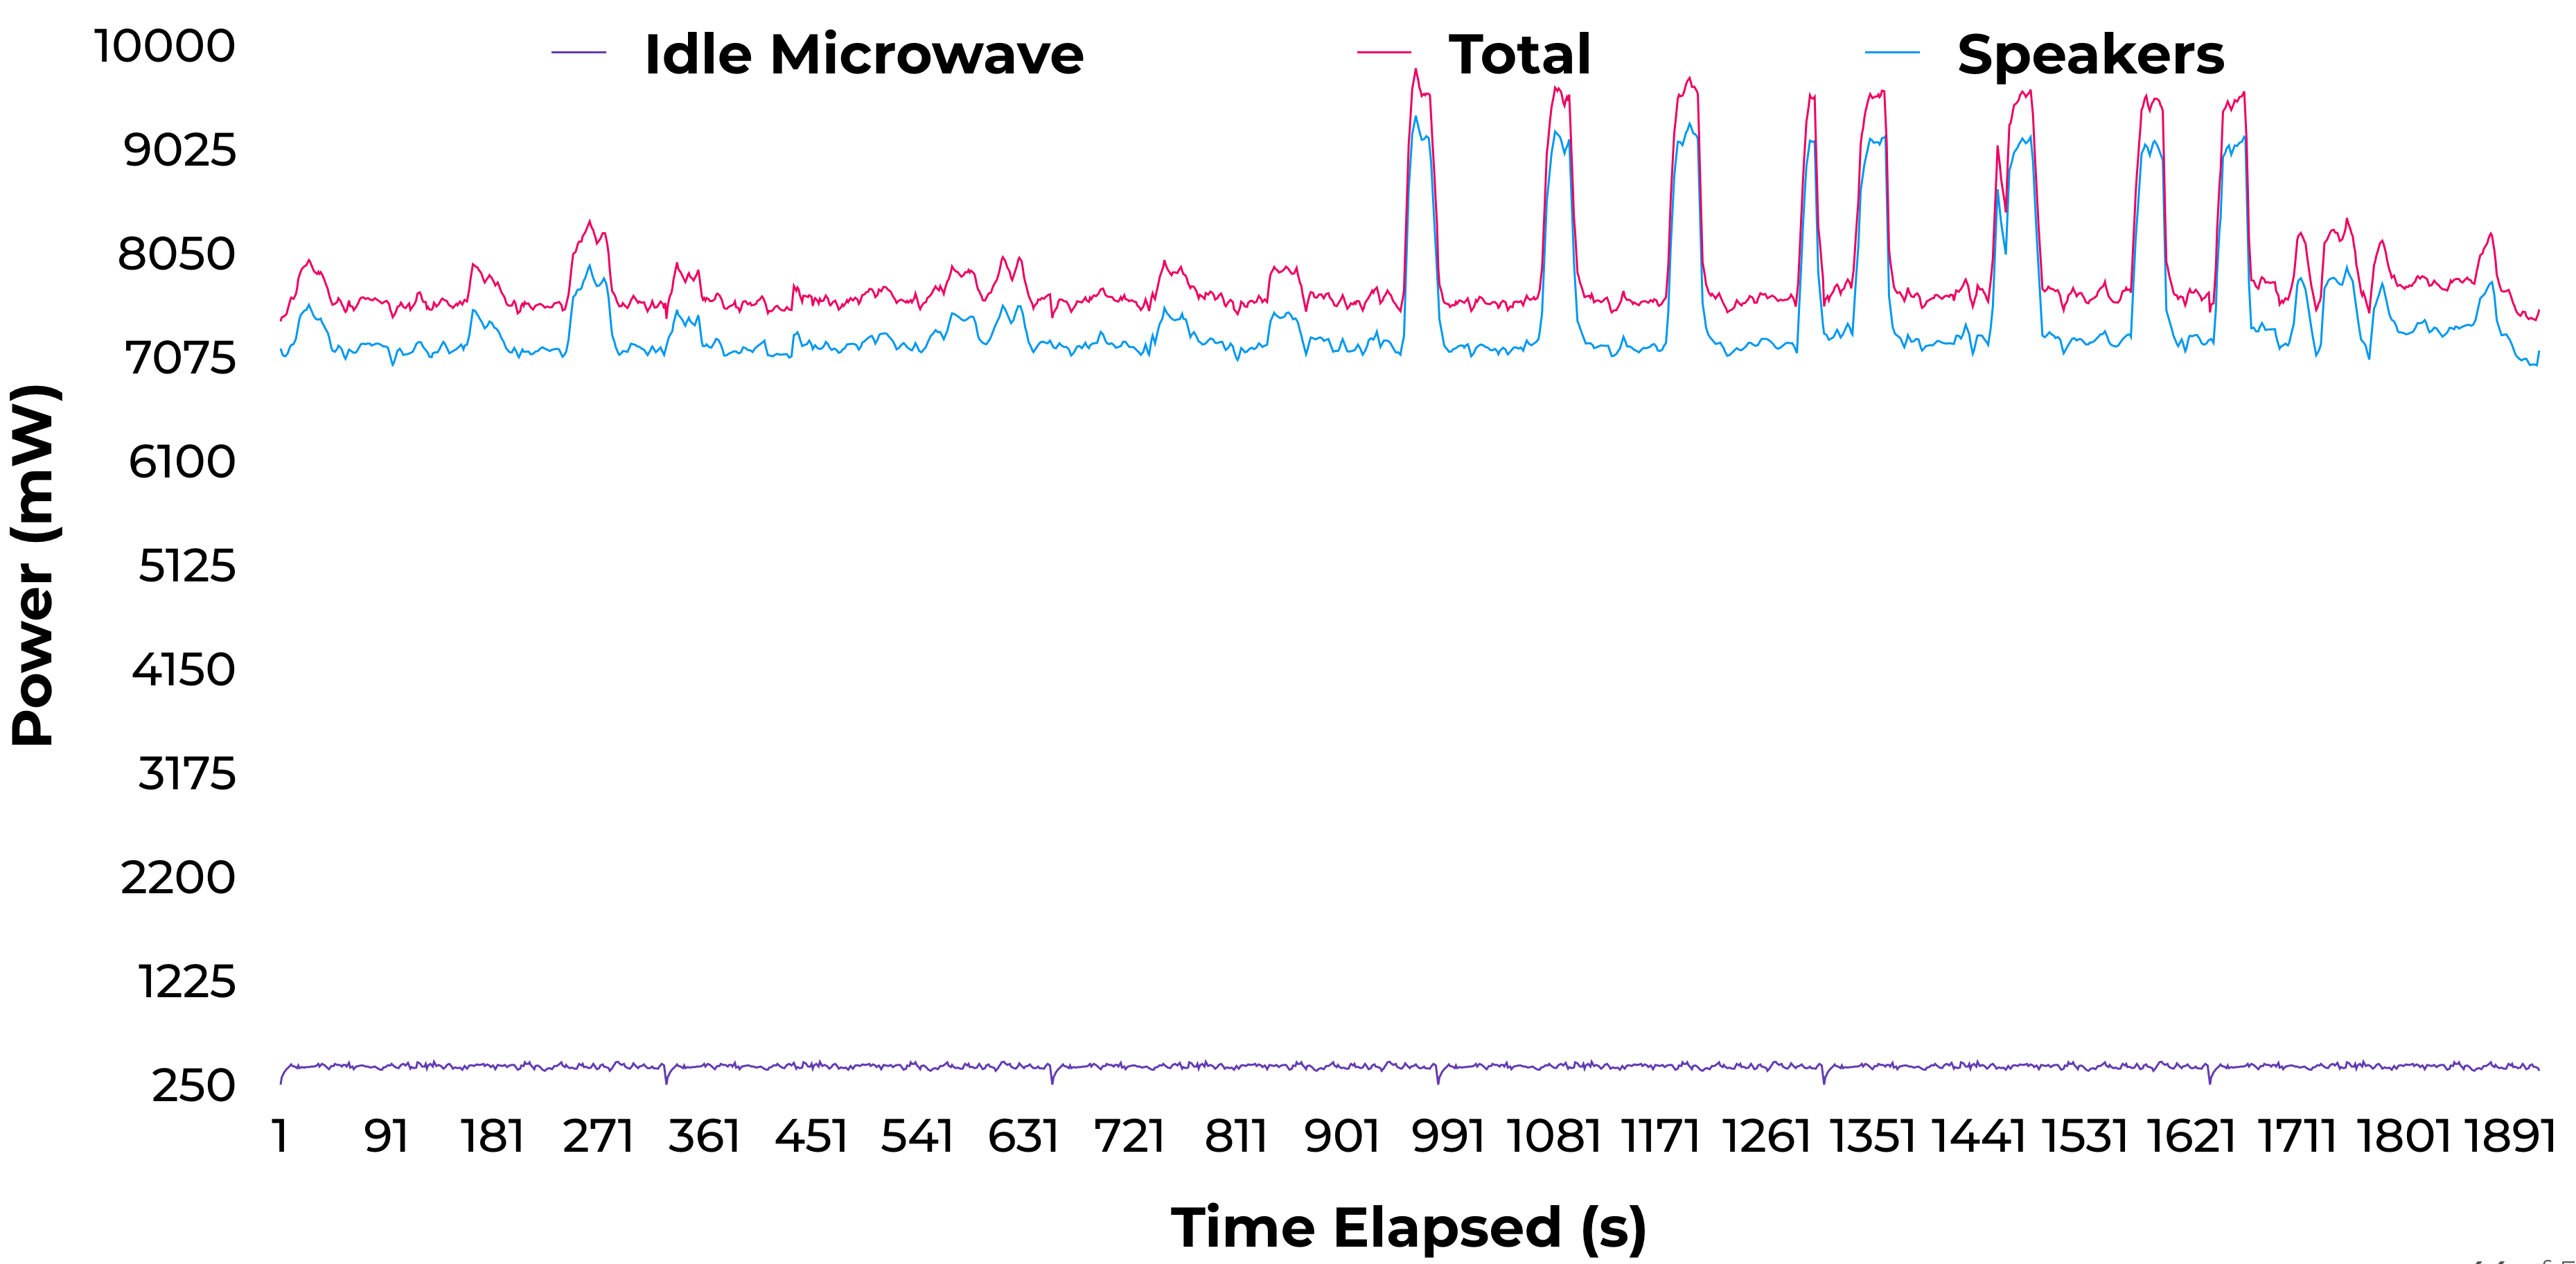
\includegraphics[width=1\textwidth]{figures/idleuWaveNoise.png}
  \caption{Idle microwave with figure \ref{fig:bestBballSum} trace.}
  \label{fig:uWaveIdle}
\end{figure}

\begin{figure}[H]
  \centering
  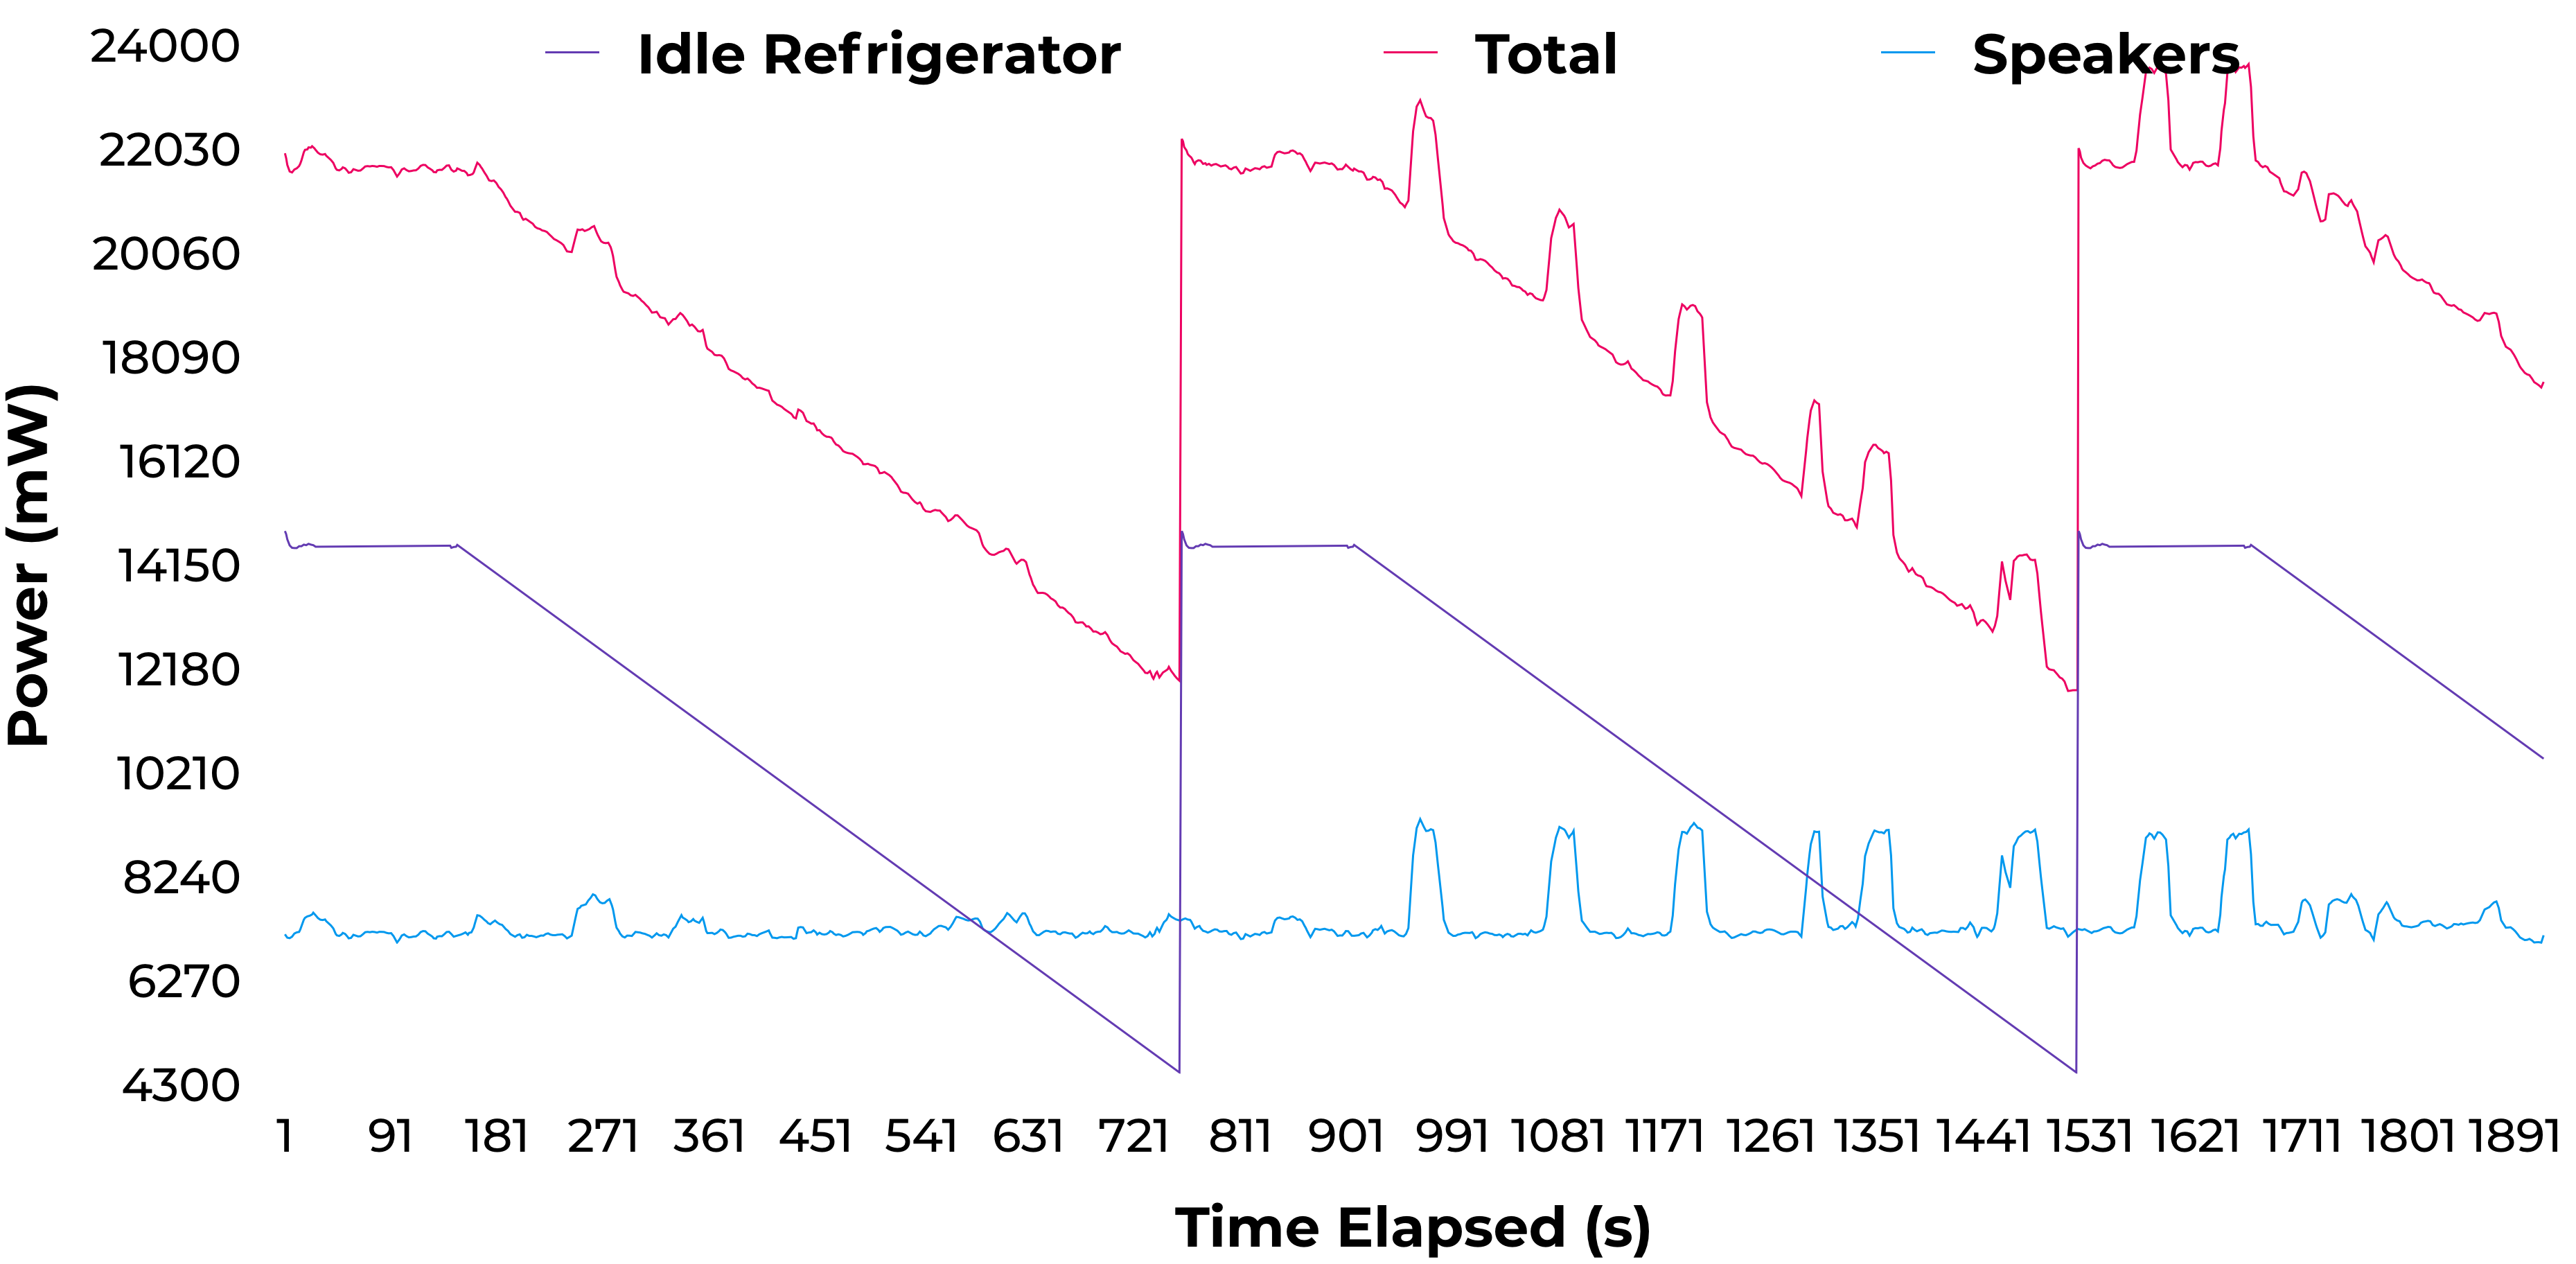
\includegraphics[width=1\textwidth]{figures/idleFridgeNoise.png}
  \caption{Idle refrigerator with figure \ref{fig:bestBballSum} trace.}
  \label{fig:fridgeIdle}
\end{figure}

\begin{figure}[H]
  \centering
  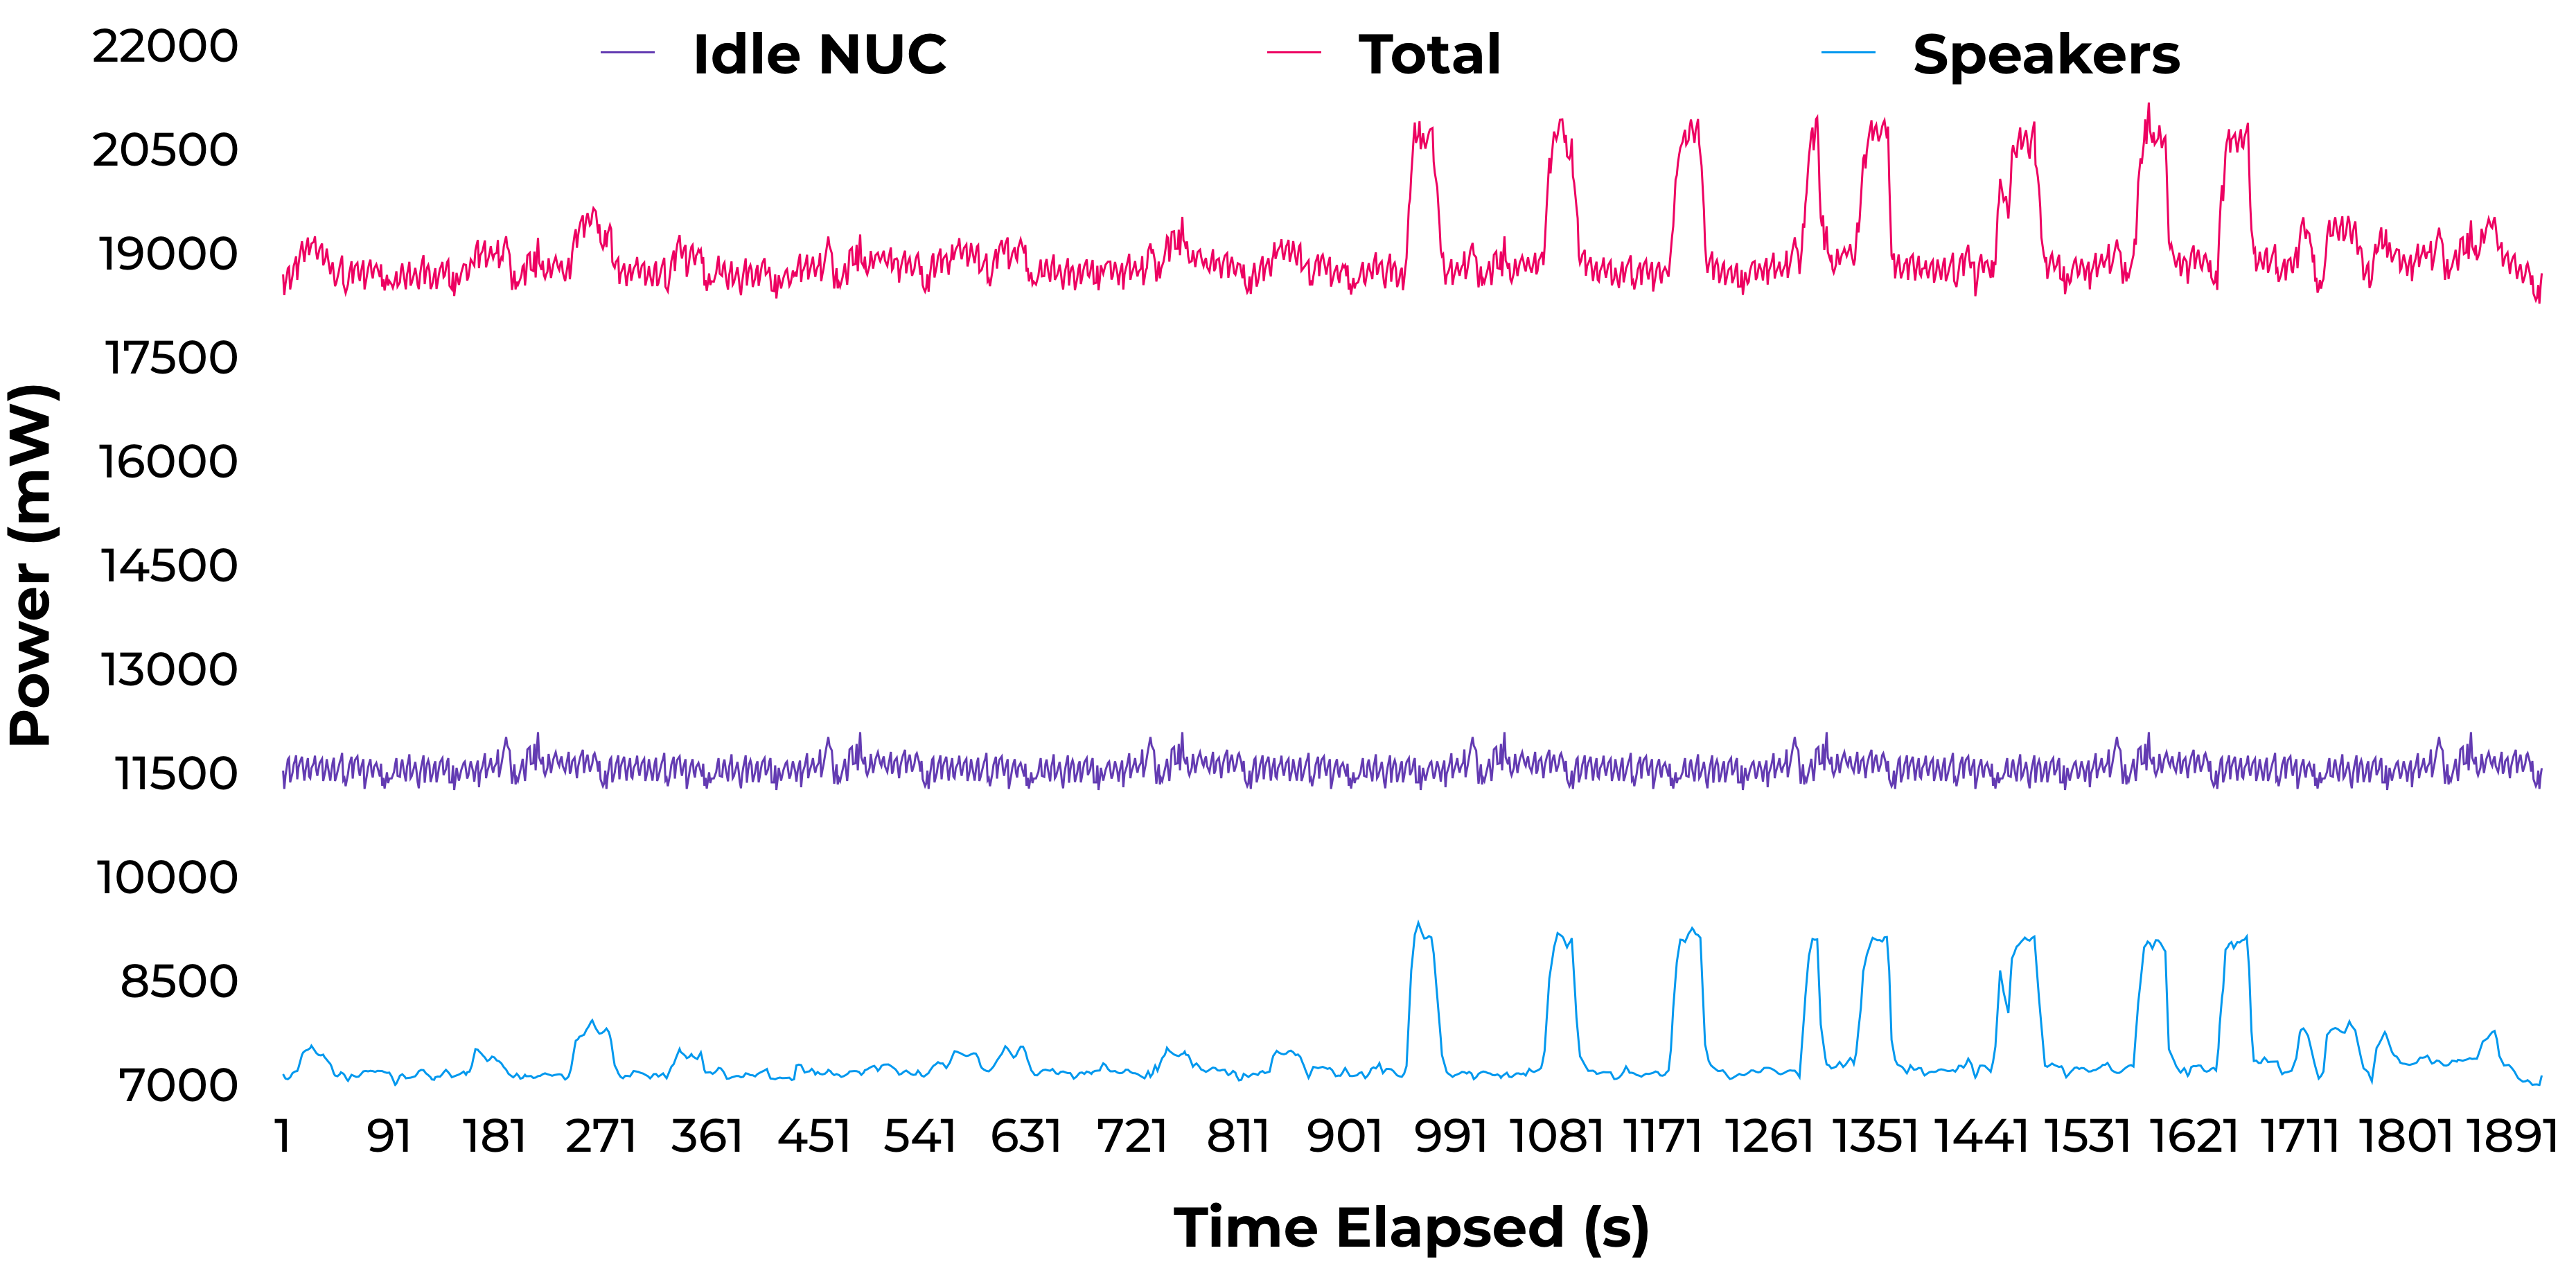
\includegraphics[width=1\textwidth]{figures/idleIntelNUCNoise.png}
  \caption{Idle PC (Intel NUC) with figure \ref{fig:bestBballSum} trace.}
  \label{fig:nucIdle}
\end{figure}

\begin{figure}[H]
    \centering
    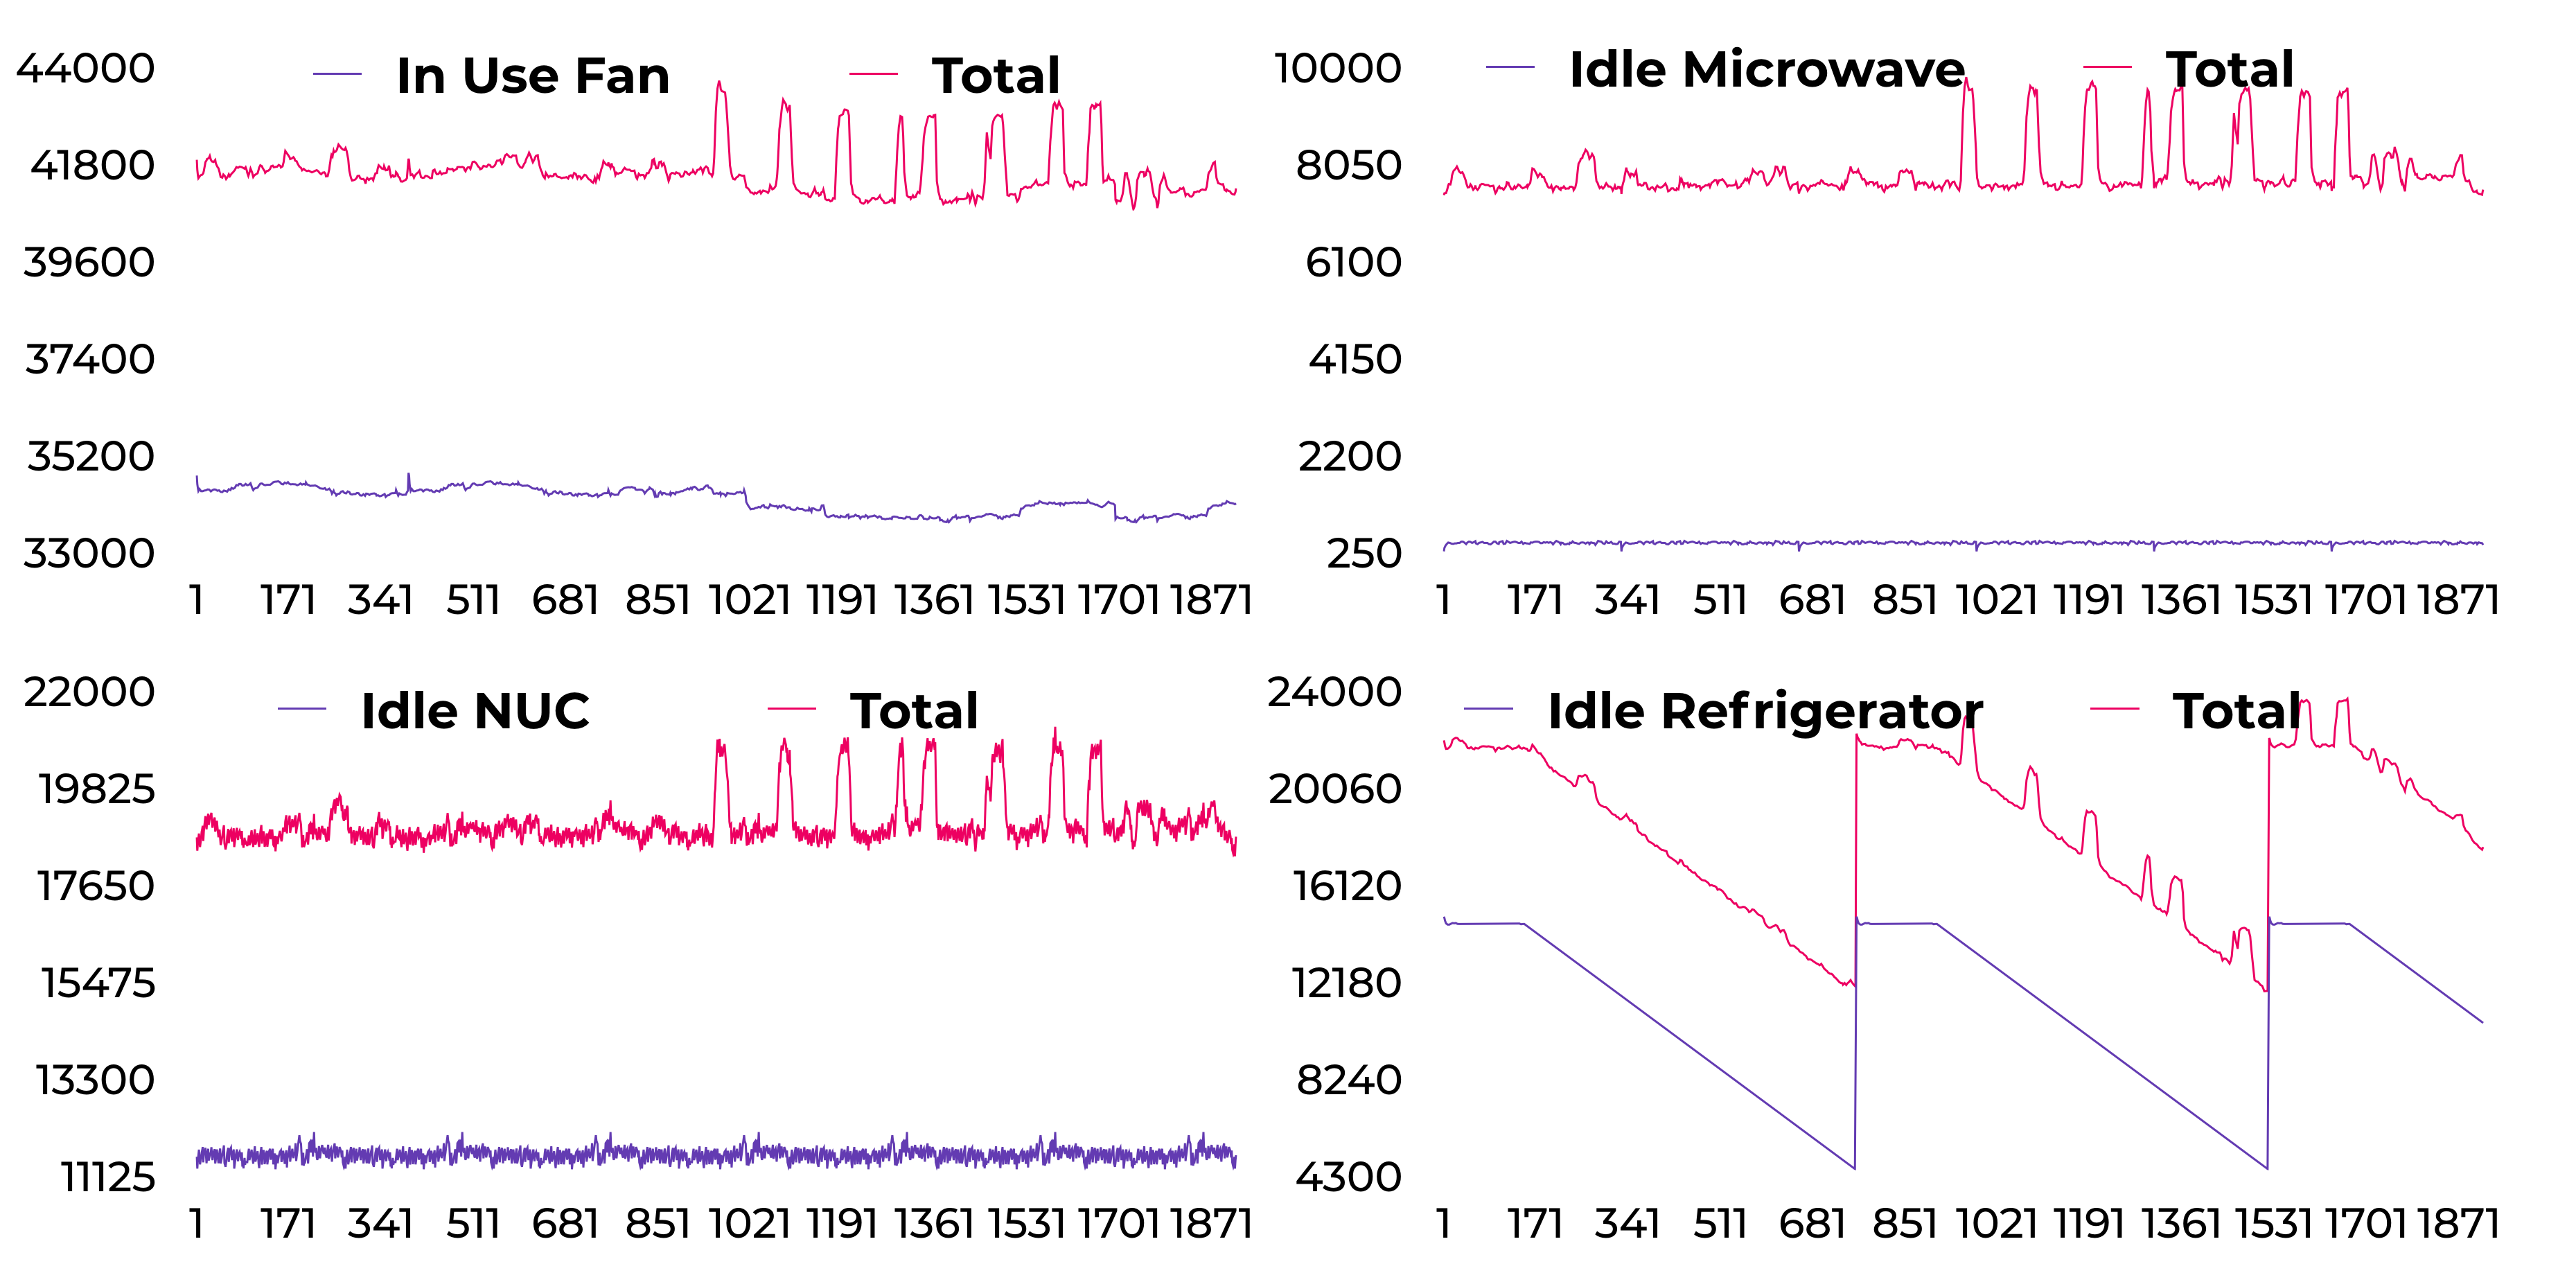
\includegraphics[width=1\textwidth]{figures/allIdleNoise.png}
    \caption{\ref{fig:fanIdle}, \ref{fig:uWaveIdle}, \ref{fig:fridgeIdle}, and \ref{fig:nucIdle} figures zoomed in}
    \label{fig:allIdleNoise}
  \end{figure}

\begin{figure}[H]
  \centering
  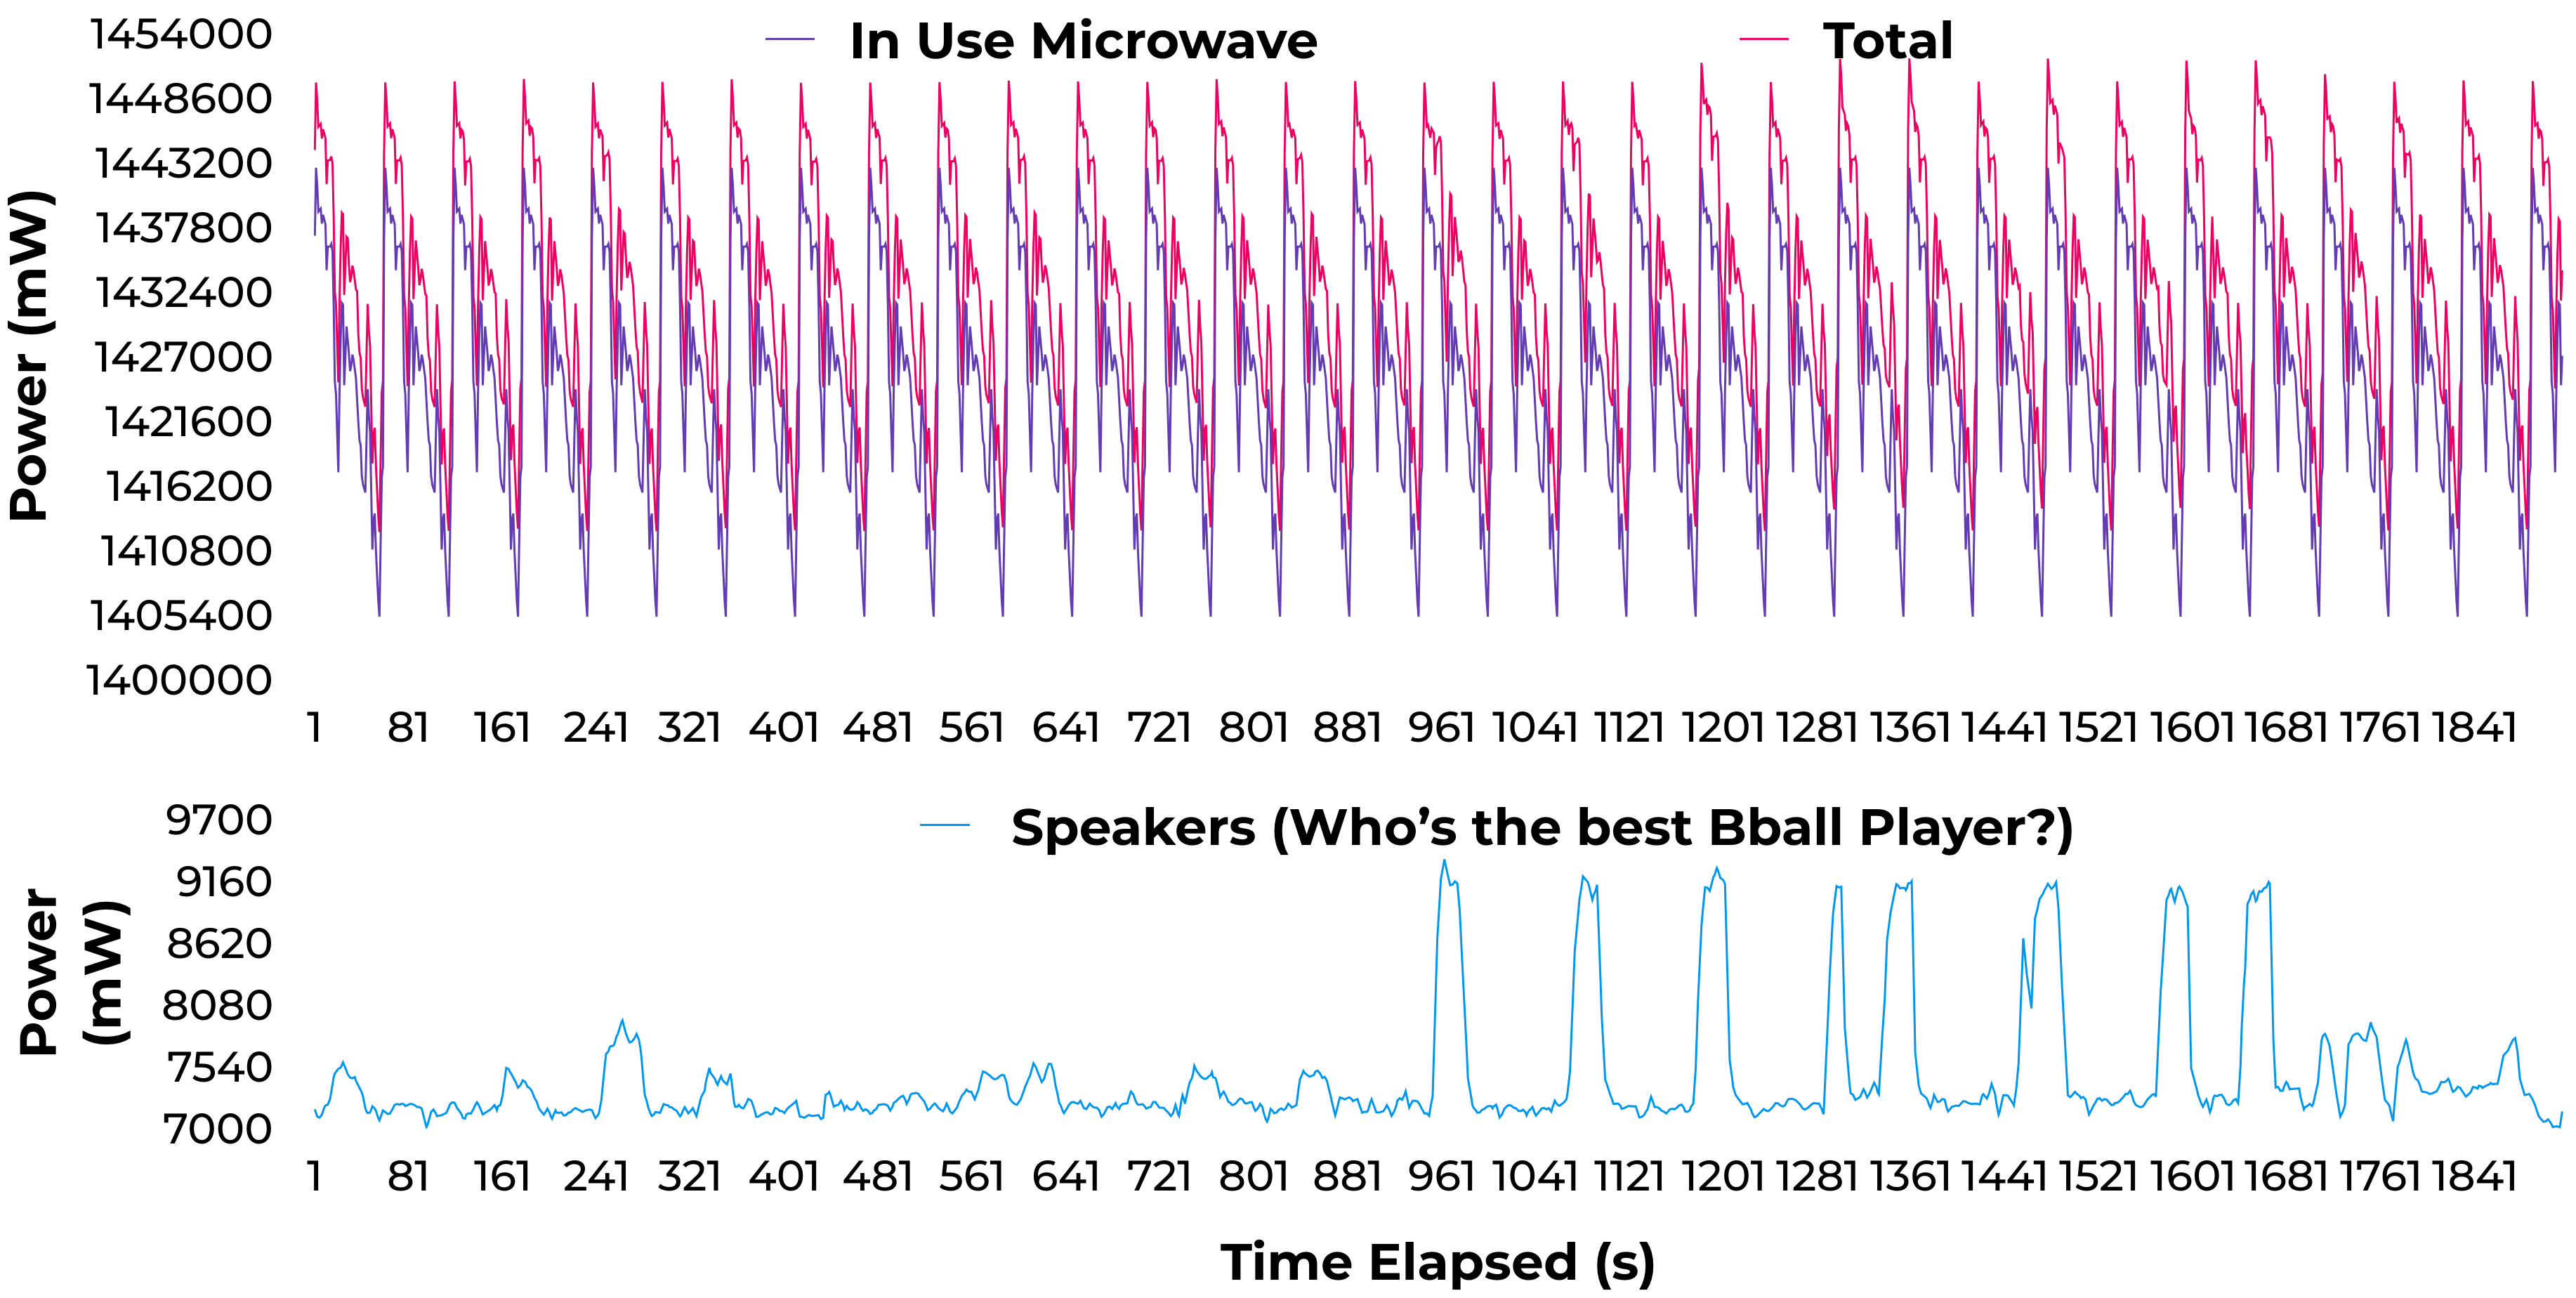
\includegraphics[width=1\textwidth]{figures/inUseuWaveNoiseSeperate.png}
  \caption{In use Microwave with figure \ref{fig:bestBballSum} trace seperately.}
  \label{fig:uWaveInUseSeperate}
\end{figure}

\begin{figure}[H]
  \centering
  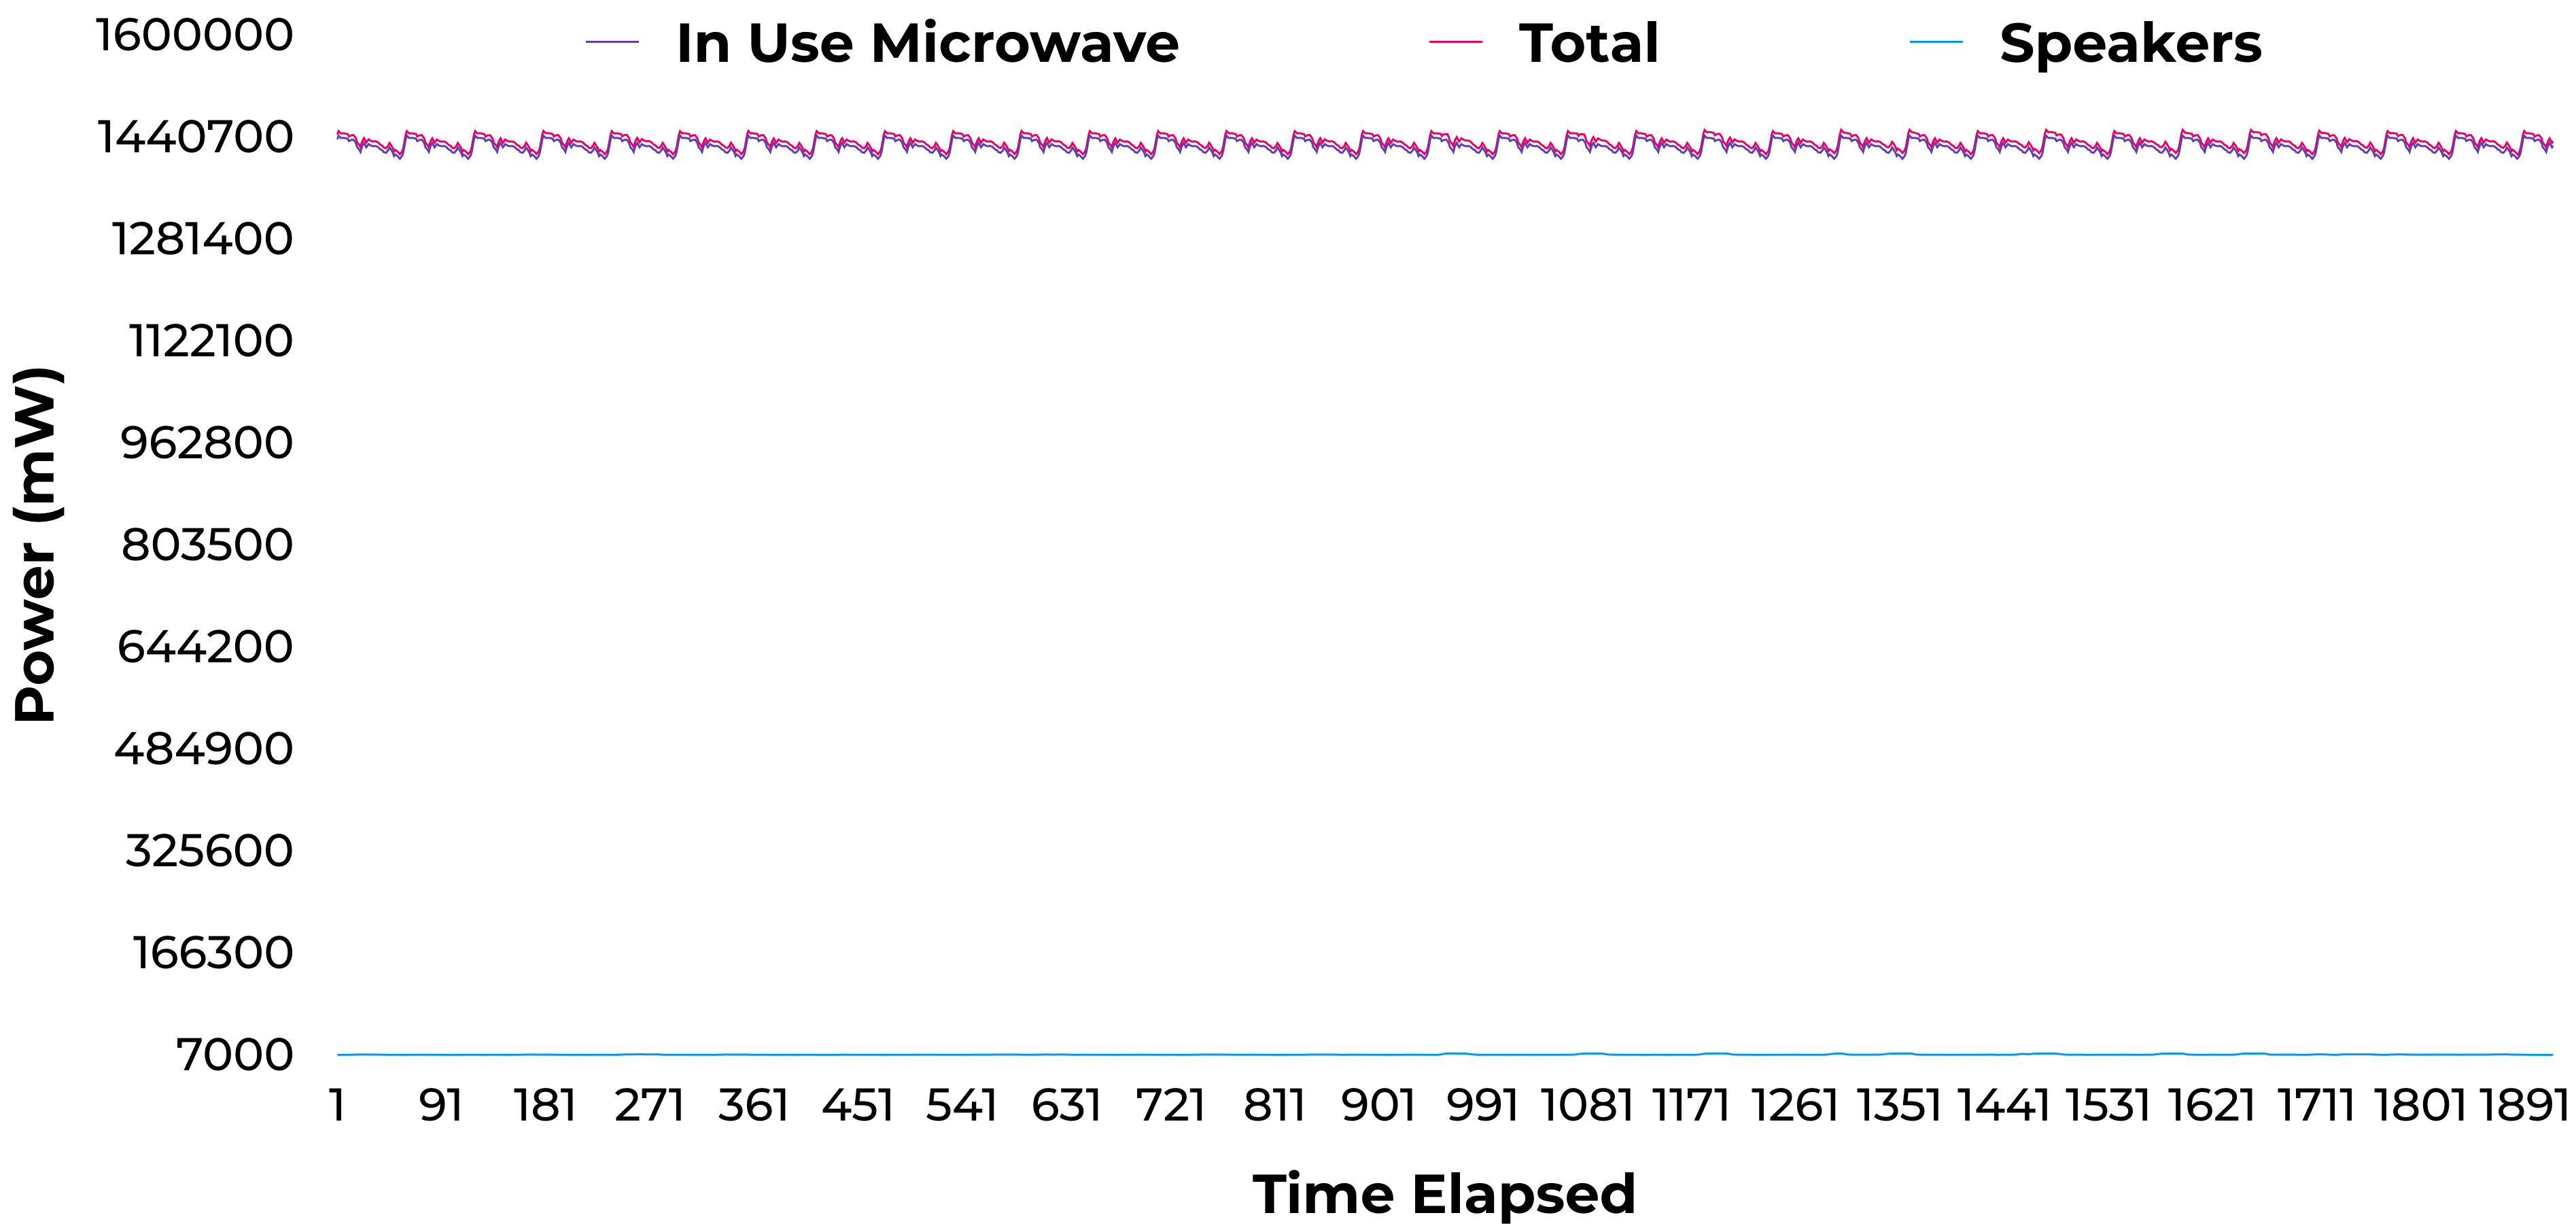
\includegraphics[width=1\textwidth]{figures/inUseuWaveNoise.png}
  \caption{In use Microwave with figure \ref{fig:bestBballSum} trace.}
  \label{fig:uWaveInUse}
\end{figure}

\begin{figure}[H]
  \centering
  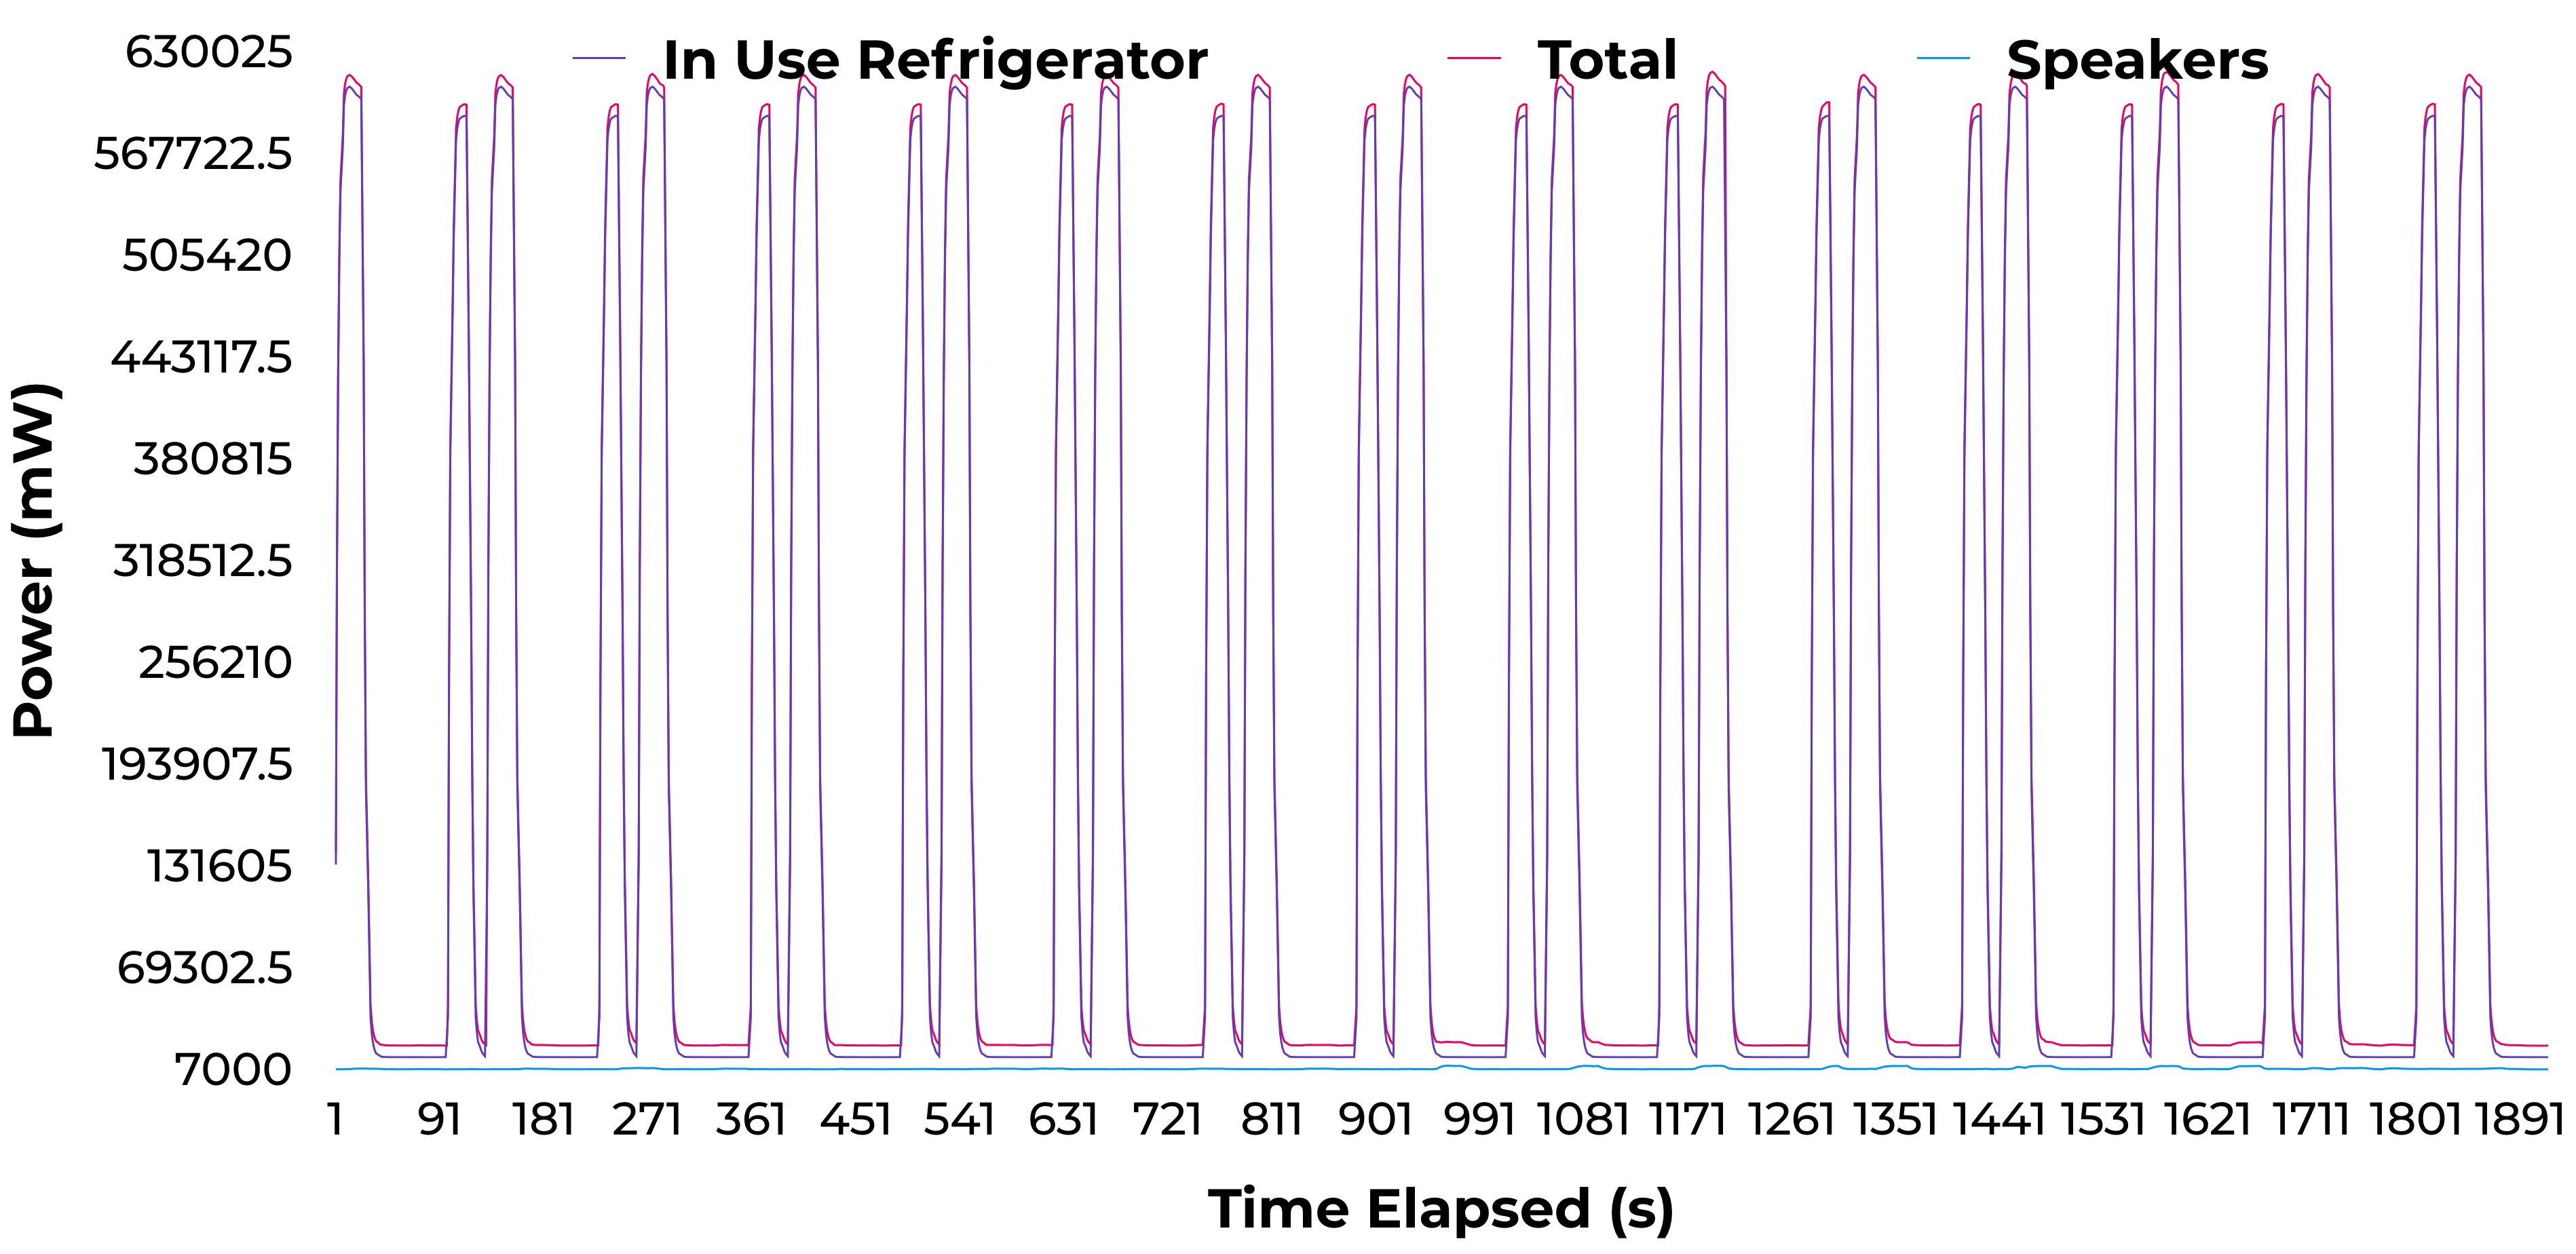
\includegraphics[width=1\textwidth]{figures/inUseFridgeNoise.png}
  \caption{Fridge in the middle of cooling with figure \ref{fig:bestBballSum} trace.}
  \label{fig:fridgeInUse}
\end{figure}

\begin{figure}[H]
  \centering
  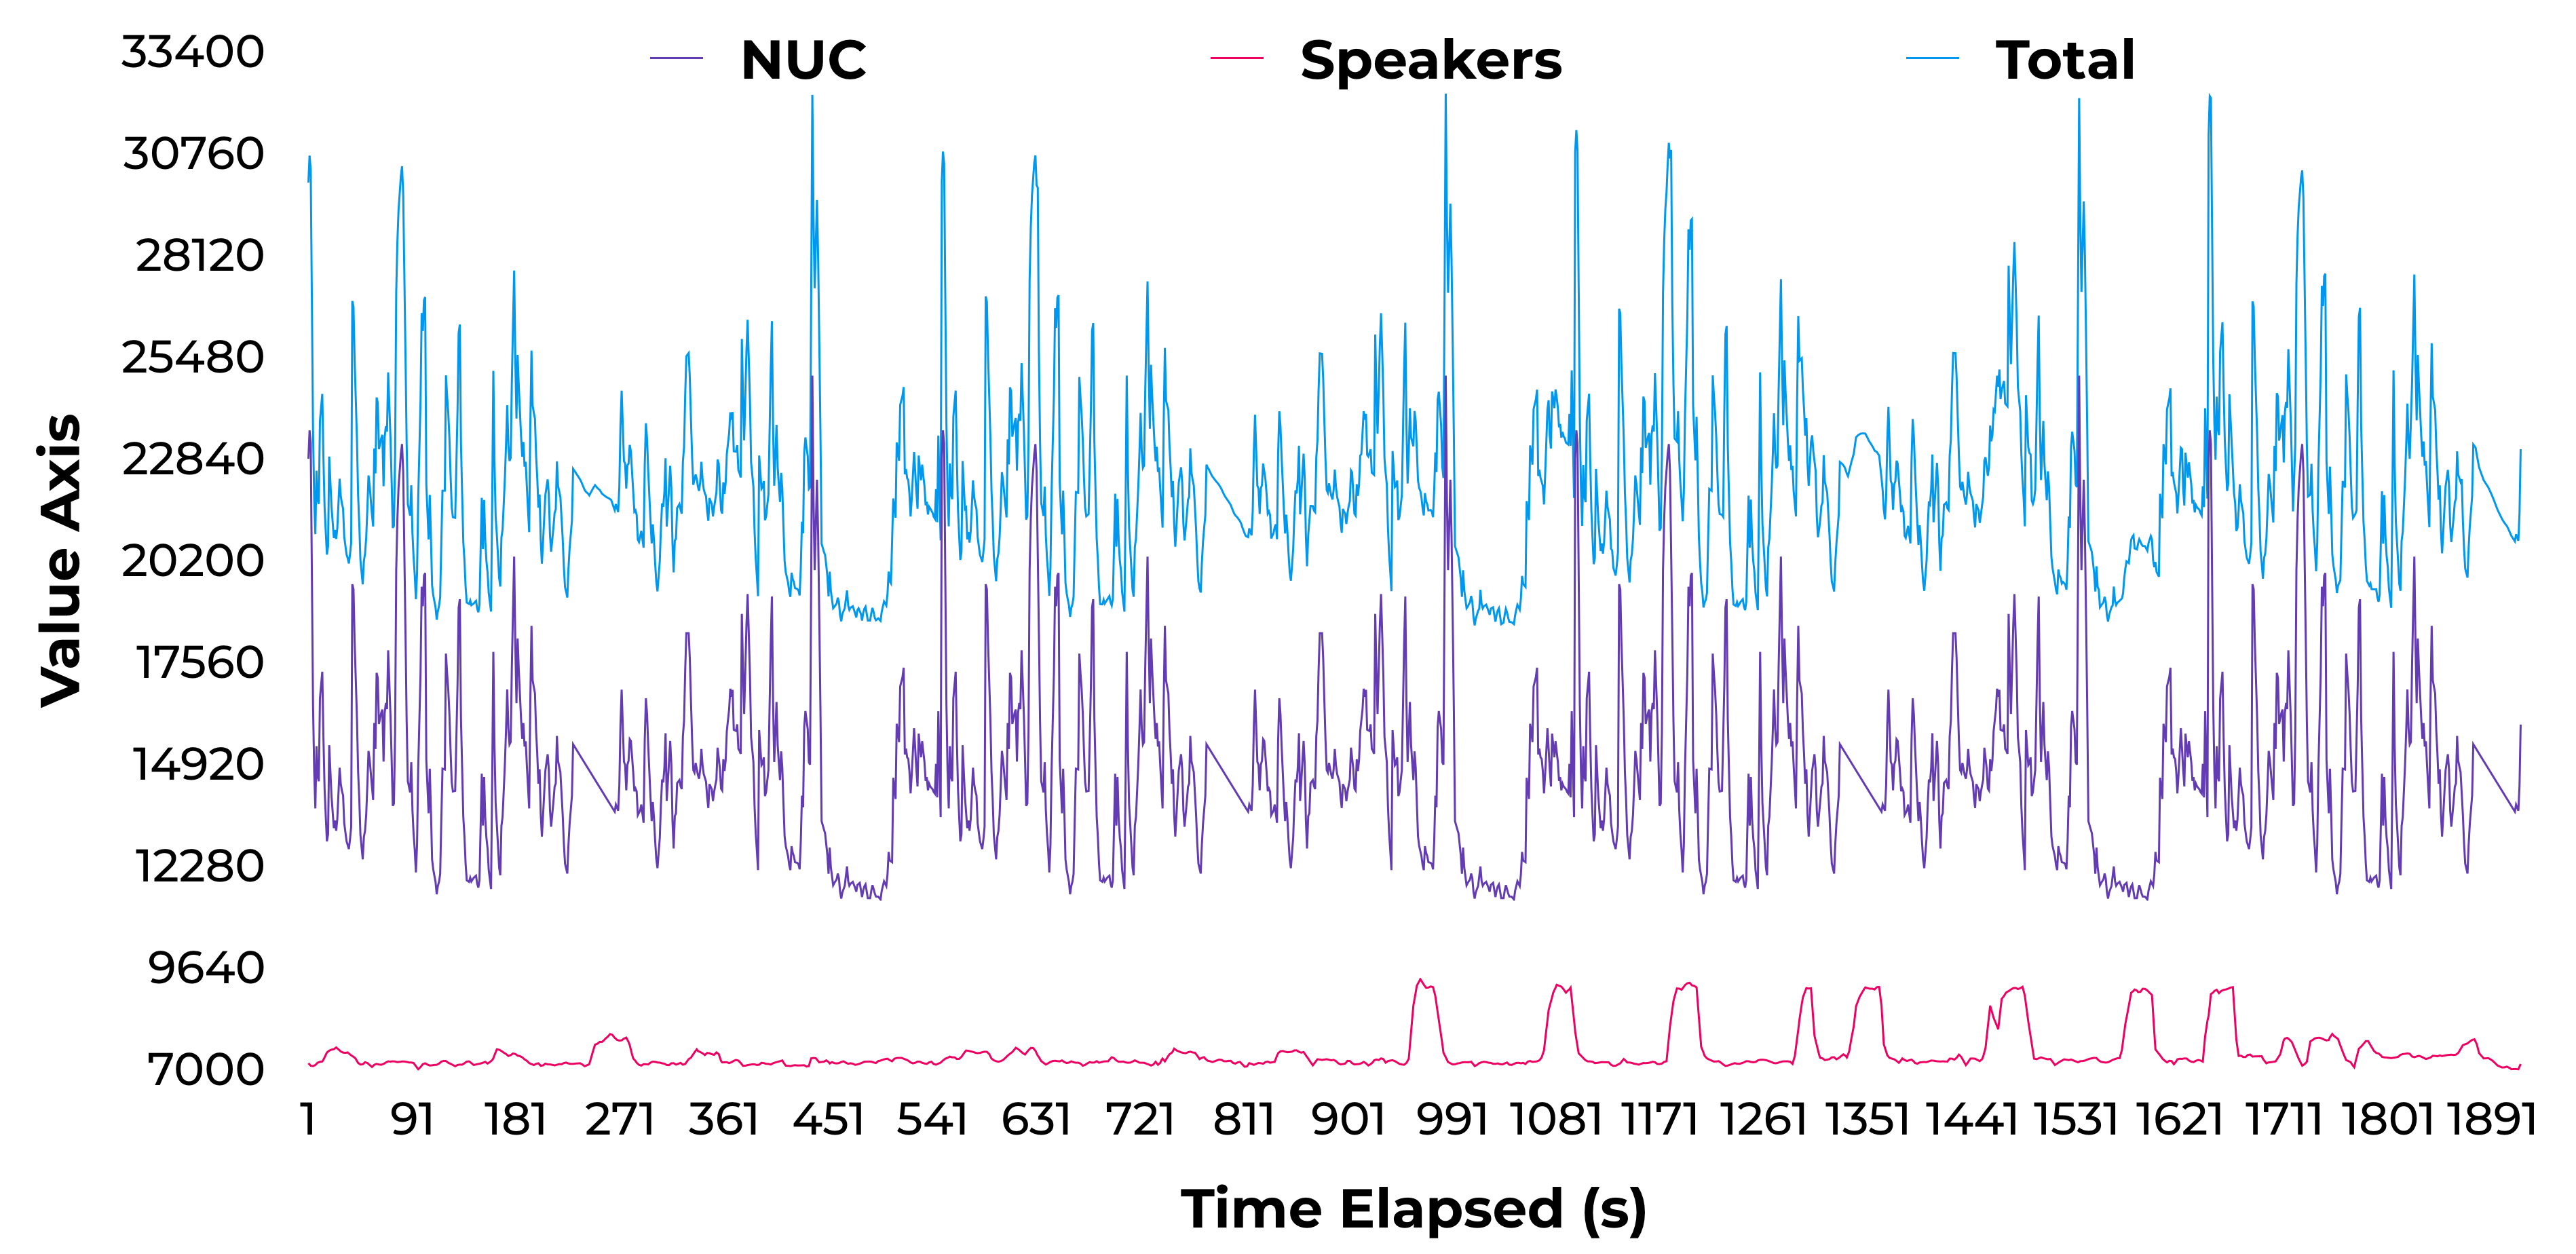
\includegraphics[width=1\textwidth]{figures/inUseNUCNoise.png}
  \caption{PC in use with figure \ref{fig:bestBballSum} trace.}
  \label{fig:nucInUse}
\end{figure}

The figures above show that it is possible to determine the smart speaker in use from visual examination of power spikes even in the presence of noise. If the noise within the house is stable, the power spikes will just be shifted up as shown in figure \ref{fig:fanIdle}. If the noise within the house is low power then, the spikes will visually overpower the noise, as shown in figure \ref{fig:nucIdle}.

But if the noise within the house is large in magnitude such as the microwave or fridge while in use \ref{fig:uWaveInUse} \ref{fig:fridgeInUse}, then the large power usage by these decices will completely squash the power spikes from the smart speakers. The spikes can no longer be seen, even when zoomed in, as shown in figure \ref{fig:uWaveInUseSeperate}. The smart speaker spikes also dissapear if the noise of a device is on the same or a larger magnitude than the power spikes, as shown in figure \ref{fig:nucInUse}. The power spikes can still be seen in the sum graph for this figure, but it would be impossible to visually differentiate between a power spike from a speaker and from the noise without knowing the original smart speaker graph.

These two cases occur depending on the house. If a lot of battery power devices such as laptops or phones are used in a house then it would would still be possible to visually determine the power spikes. Or in another case, if high power devices such as the microwave or fridge are not in use often, then the smart speaker spikes can be visually correlated. But if a household has a lot of devices plugged into an outlet for power, then the smart speaker power spikes will dissapear in the cumalative nosie of all the devices. In the first case, there are privacy implications in what could be learned from a household's power line information, which are easily accessible in most households today \cite{griffith_2017}.

\section{Smart Speaker Comparison}
\label{smartSpeakerComparisonSection}
The figures in section \ref{sumPowerGraph} show that the Echo Dot uses a lot more energy than the other smart speakers. Because of this, we wanted to compare the energy and network usages of the three smart speakers individually so that we can determine trade-offs that they make.

In the graphs below, we display power and network traces for the echo dot 1, Eufy genie 1, and Google home. We used the same time frame as the graph in figure \ref{fig:bestBballSeperate} for the two graphs below. We removed the second Echo Dot and Eufy Genie for simplicity.

In the same time frame as the two graphs below, we also recorded the average power usage and throughput for the smart speakers. For average power, from greatest to least, we have the Echo Dot (1650 mW), Eufy Genie (1325 mW), Google Home (1175 mW). For average throughput, from greatest to least, we have the Eufy Genie (1743 bytes), Google Home (800 bytes), Echo Dot (325 bytes).

\begin{figure}[H]
  \centering
  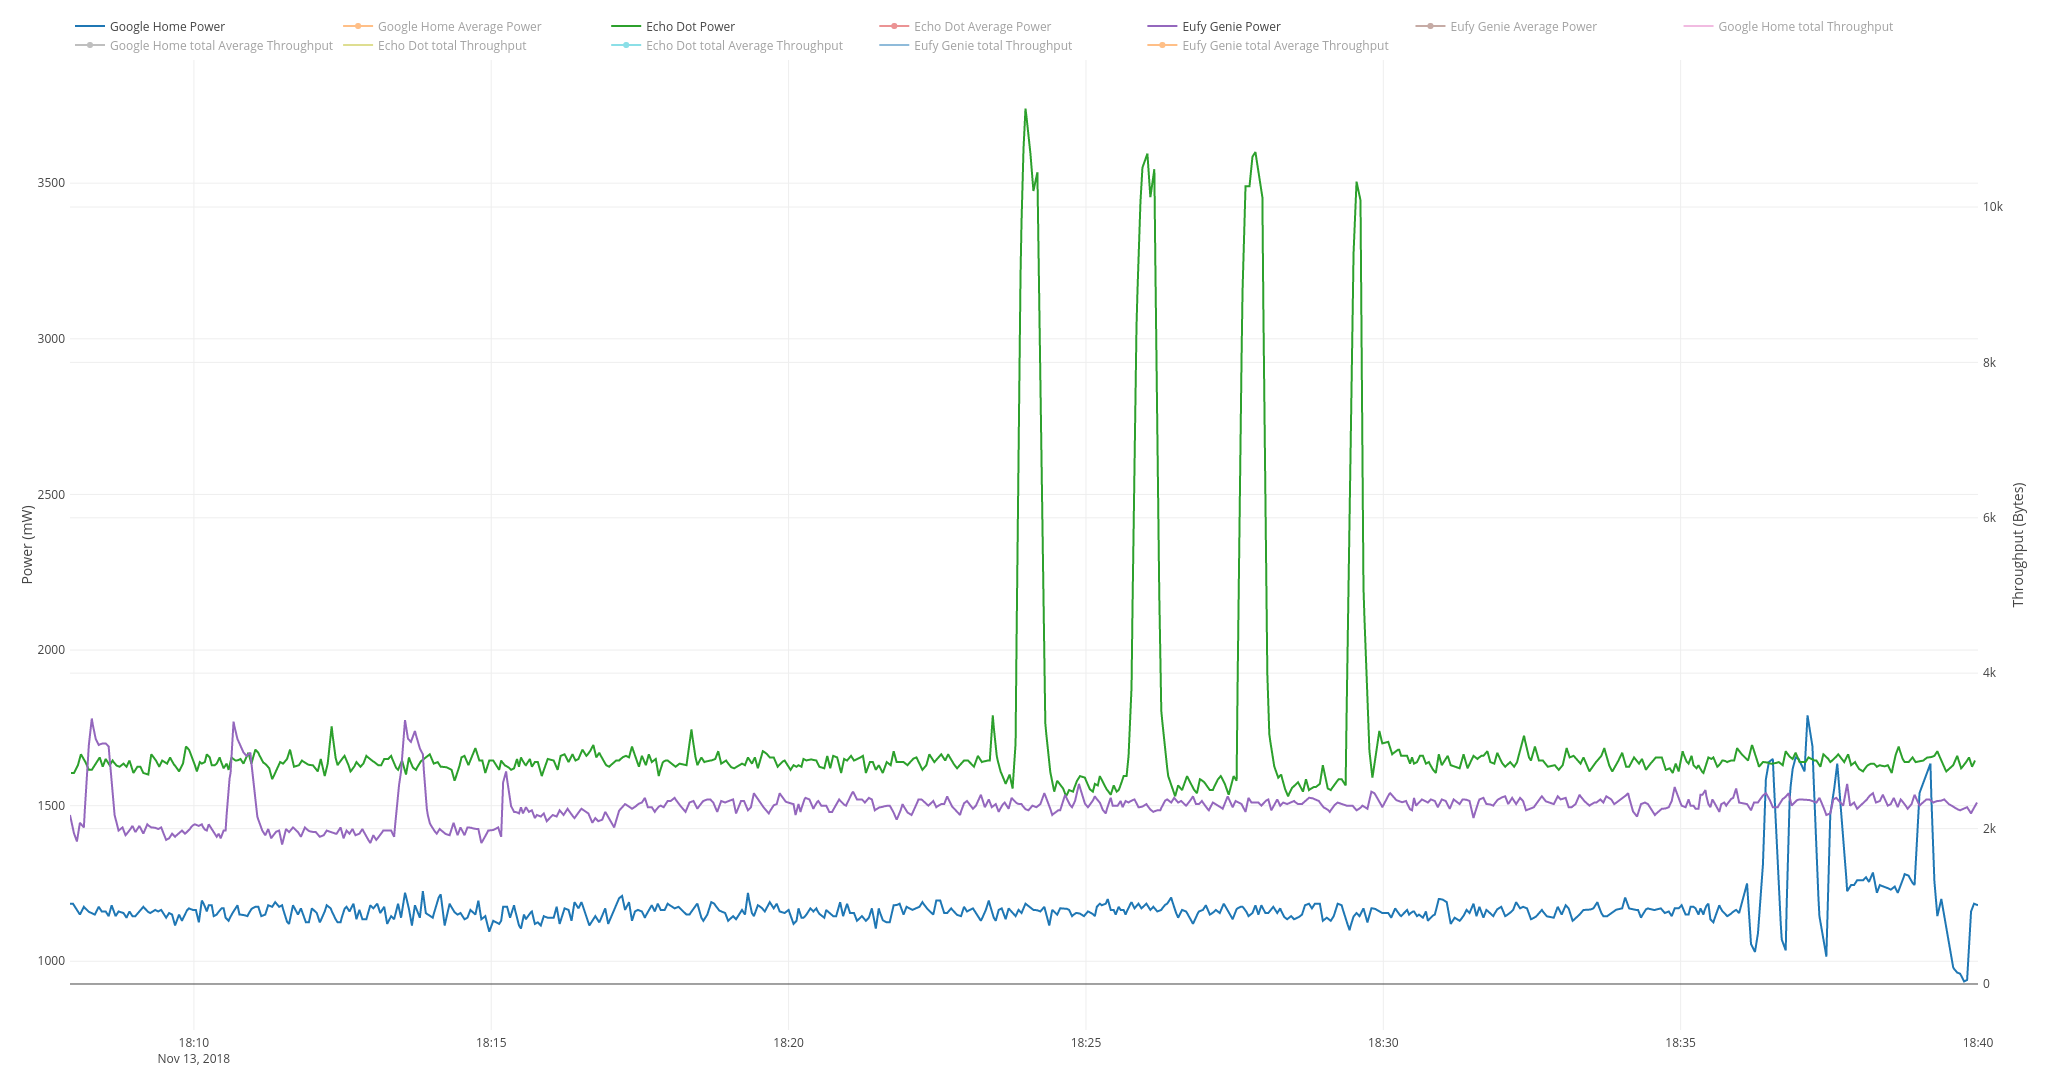
\includegraphics[width=1\textwidth]{figures/smartSpeakerSeperate.png}
  \caption{Power usage of Echo Dot 1, Eufy Genie 1, and Google Home over time when asked ``who is the best basketball player''. Same graph as figure \ref{fig:bestBballSeperate} with Echo Dot 2 and Eufy Genie removed.}
  \label{fig:smartSpeakerSeperate}
\end{figure}

\begin{figure}[H]
  \centering
  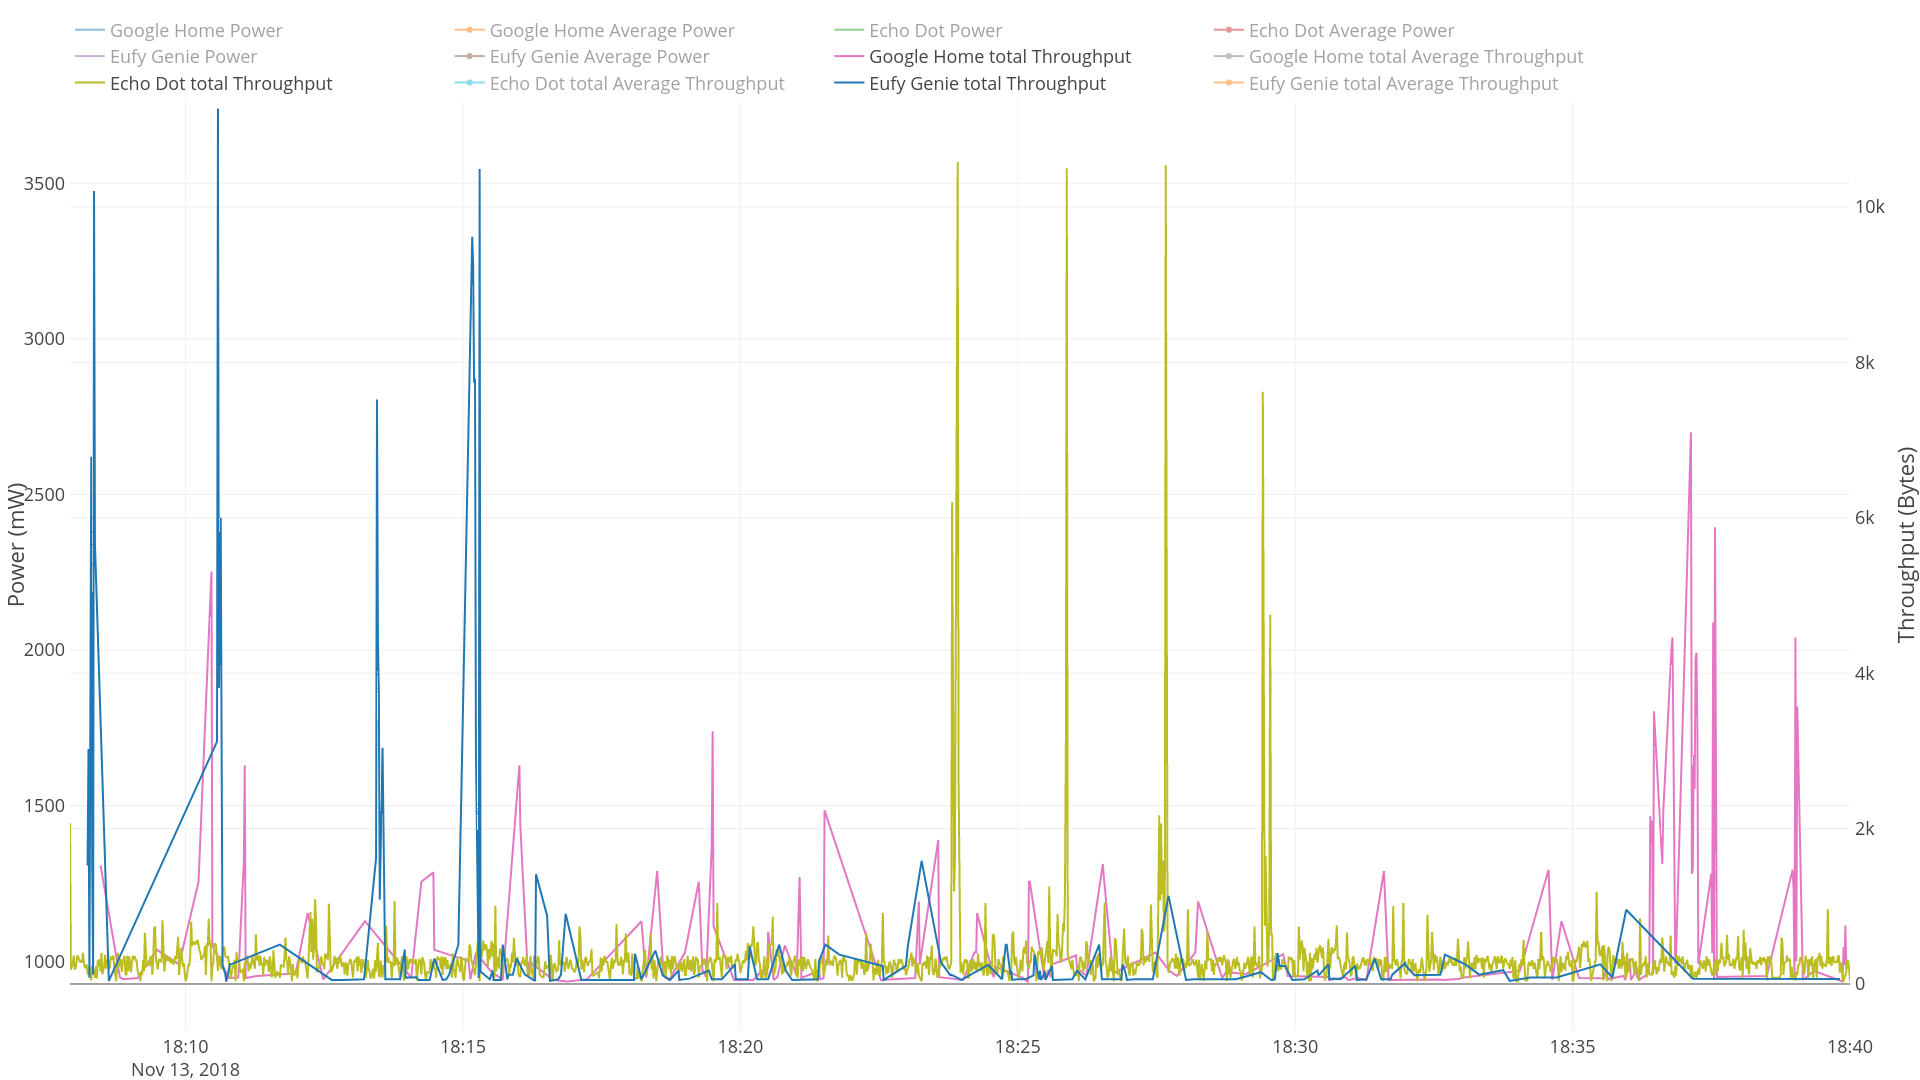
\includegraphics[width=1\textwidth]{figures/smartSpeakerNetworkSeperate.png}
  \caption{Power usage of Echo Dot 1, Eufy Genie 1, and Google Home over time when asked ``who is the best basketball player''. Same time frame as figure \ref{fig:smartSpeakerSeperate}}
  \label{fig:smartSpeakerNetworkSeperate}
\end{figure}

Finally, we noticed that the Echo Dot is characterized by a power spike that is a lot larger than the other smart speakers and wer interested to see what trade-offs these devices made.

From the results in section \ref{smartSpeakerComparisonSection}, we can see that the echo uses the most power, then the Eufy, then the Google Home. However, the Eufy uses the most network throughput, then the Google Home, then the Echo Dot. We believe the Eufy is constantly communicating through the network so that it can cache results, minimizing onboard operations. The Echo Dot, on the other hand, uses the least network throughput and opts to do as much on board work as possible. The Google Home sits in the middle, querying the network, for more relevant things that it can cache for when the user asks the questions. It seems they pre-request results better. It is interesting that the Google Home still sits in the middle for network throughput when it is the only one that sends UPnP at such a high frequency. However, this is mostly speculation and would be interesting to see more research on this.

From the results in section \ref{smartSpeakerComparisonSection}, we can see that the echo uses the most power, then the Eufy, then the Google Home. However, the Eufy uses the most network throughput, then the Google Home, then the Echo Dot. We believe the Eufy is constantly communicating through the network so that it can cache results, minimizing onboard operations. The Echo Dot, on the other hand, uses the least network throughput and opts to do as much on board work as possible. The Google Home sits in the middle, querying the network, for more relevant things that it can cache for when the user asks the questions. It seems they pre-request results better. It is interesting that the Google Home still sits in the middle for network throughput when it is the only one that sends UPnP at such a high frequency. However, this is mostly speculation and would be interesting to see more research on this.